\chapter{Introduction}

  \section{The chemical perception}
  The chemical senses are one the oldest sensory system \cite{yohe2018evolutionary}. They are the most used sensory modality and observed in a wide range of taxa, from unicellular \cite{bardwell2005walk} to mammalian. Some features and basics principles are highly conservated across phyla \cite{hildebrand1997mechanisms,yarmolinsky2009common}, and mediate several behaviors like predator avoidance, food-finding, and mating necessary to the survival of any species.

  Fish are immersed in a complex chemical environment at any time and have evolved a refined sensory system to perceived and interpret these chemical stimuli. For fish, chemical perception is mediated by three senses: olfaction (smell), gustation (taste), and a common chemical sense. Unlike terrestrial species, where substances perceived by smell and taste differ by the medium of transport of the molecules, fish taste and smell through the same medium: water. The solubility of compounds in water determines the type of compounds that can be transported and perceived. Therefore, chemical perception is non-directional and persistent. The distance traveled and the perceived concentration depend on the diffusion and convection of the medium, determining the perception threshold and the compound's residence time in the environment. The chemical perception is extremely specific, being contained in the molecular structures and the complex mixture of chemicals.

  Mechanisms of perception have been well studied for diverse fish species \cite{hara2012fish}, but highly complex directed behaviors like homing migration or food-finding are still poorly understood \cite{hansen2004chemosensory}. For example, fish can find food in complex environments like turbid and turbulent waters, where the perception is fragmented. Deciphering these mechanisms and their associated neural mechanisms will significantly advance the comprehension of the animal kingdom's most used sensory modality.

  One fish species, the zebrafish, is an emerging model for studying goal-driven behaviors. At the larval stage (6 days post-fertilization), the animal is transparent, and it is possible to observe the brain activity with cellular resolution using light-sheet microscopy \cite{panier2013fast}. The development of virtual reality assays makes it technically possible to associate some neuronal networks' activity to the observed behavior. Using this technique; it was possible to gain insights into several behaviors, such as prey capture \cite{bianco2011prey}, optomotor response \cite{naumann2016whole}, phototaxis \cite{wolf2017sensorimotor}, rheotaxis \cite{olive2016rheotaxis}, and thermotaxis\cite{haesemeyer2019convergent}.

  The development and functioning of the fish sensory organs, particularly in the zebrafish, have been well characterized. However, there are few behavioral studies on chemical perception and chemically-oriented navigation. Several milestones have to be achieved before using virtual reality assays to study chemically-driven navigation. One needs to find and characterize products that elicit robust and attractive behaviors. The space of possibilities is vast, and completing this task will necessitate a high-throughput setup to explore combinations of products, concentrations, and fish ages. In a second time, when a product that elicits a robust and attractive response will be characterized, studying realistic chemically-driven navigation will require a setup capable of reproducing turbulent flows where the fish is immersed and submitted to a complex chemical environment with fragmented perception.

  In the next sections, we will present the fish's sensory organs and review experimental setups used in the literature to characterize the zebrafish's chemical perception at the larval and adult stage. Then we will present two experimental setups that we built to study the chemical perception of zebrafish. Finally, we will present and discuss some results that we obtain using these setups.


    \subsection{Olfaction}
    The olfactory organ of the fish, see Figure~\ref{olfactory_schematic}, consists of two structures located in the animal's snout \cite{hara2012fish}. Each structure consists of a cavity called the olfactory chamber connected to the outside by an entrance and an exit nostril. The inside of the olfactory chamber is lined with the olfactory rosette consisting of two rows of olfactory lamellae. The olfactory epithelium, where the olfactory receptors are located, is placed on these lamellae. The olfactory organ's exact organization and position can vary depending on the fish species, for example, with the addition of a ventilation cavity as an extension of the olfactory cavity.

    \begin{figure}[h]
      \centering
      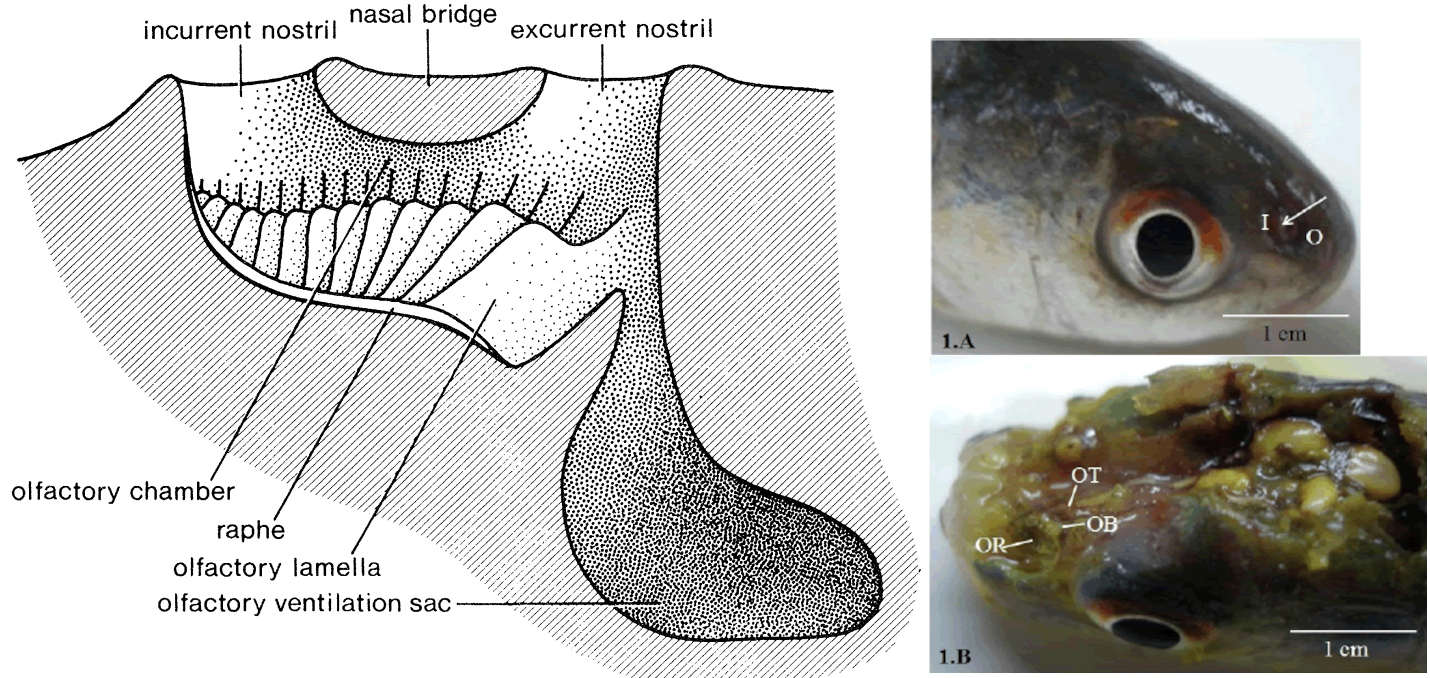
\includegraphics[width=10cm]{part_2/assets/olfactory_schematic.png}
      \caption{Olfactory system, reproduced from \cite{hara2012fish}. The olfactory organ of \textit{Labeo bata} reproduced from \cite{samajdar2016histological}, (I) is the inlet and (O) the outled channel, (OR) olfactory epithelium, (OT) olfactory tract and (OB) olfactory bulb.}
      \label{olfactory_schematic}
    \end{figure}


    The olfactory epithelium has a $100\mu m$ thick pseudostratified columnar structure \cite{hara2012fish}. It can be separated into a sensory and a non-sensory epithelium. The sensory epithelium consists of three types of cells: receptor, supporting, and basal cells; the non-sensory epithelium of goblet cells and non-sensory ciliated cells. There are five receptor cells implicated in the olfactory perception: ciliated cells, microvillous cells, crypt cells \cite{ichikawa1977fine,hansen2005diversity}, kappe cells \cite{ahuja2014kappe}, and pear-shaped cells \cite{wakisaka2017adenosine}. They express olfactory receptors of the OR, V1R, V2R, and TAAR families. Receptor cells have various sizes, shapes, and distribution inside the epithelium, see Figure~\ref{olfactory_schematic_full}.

    \begin{figure}[h]
      \centering
      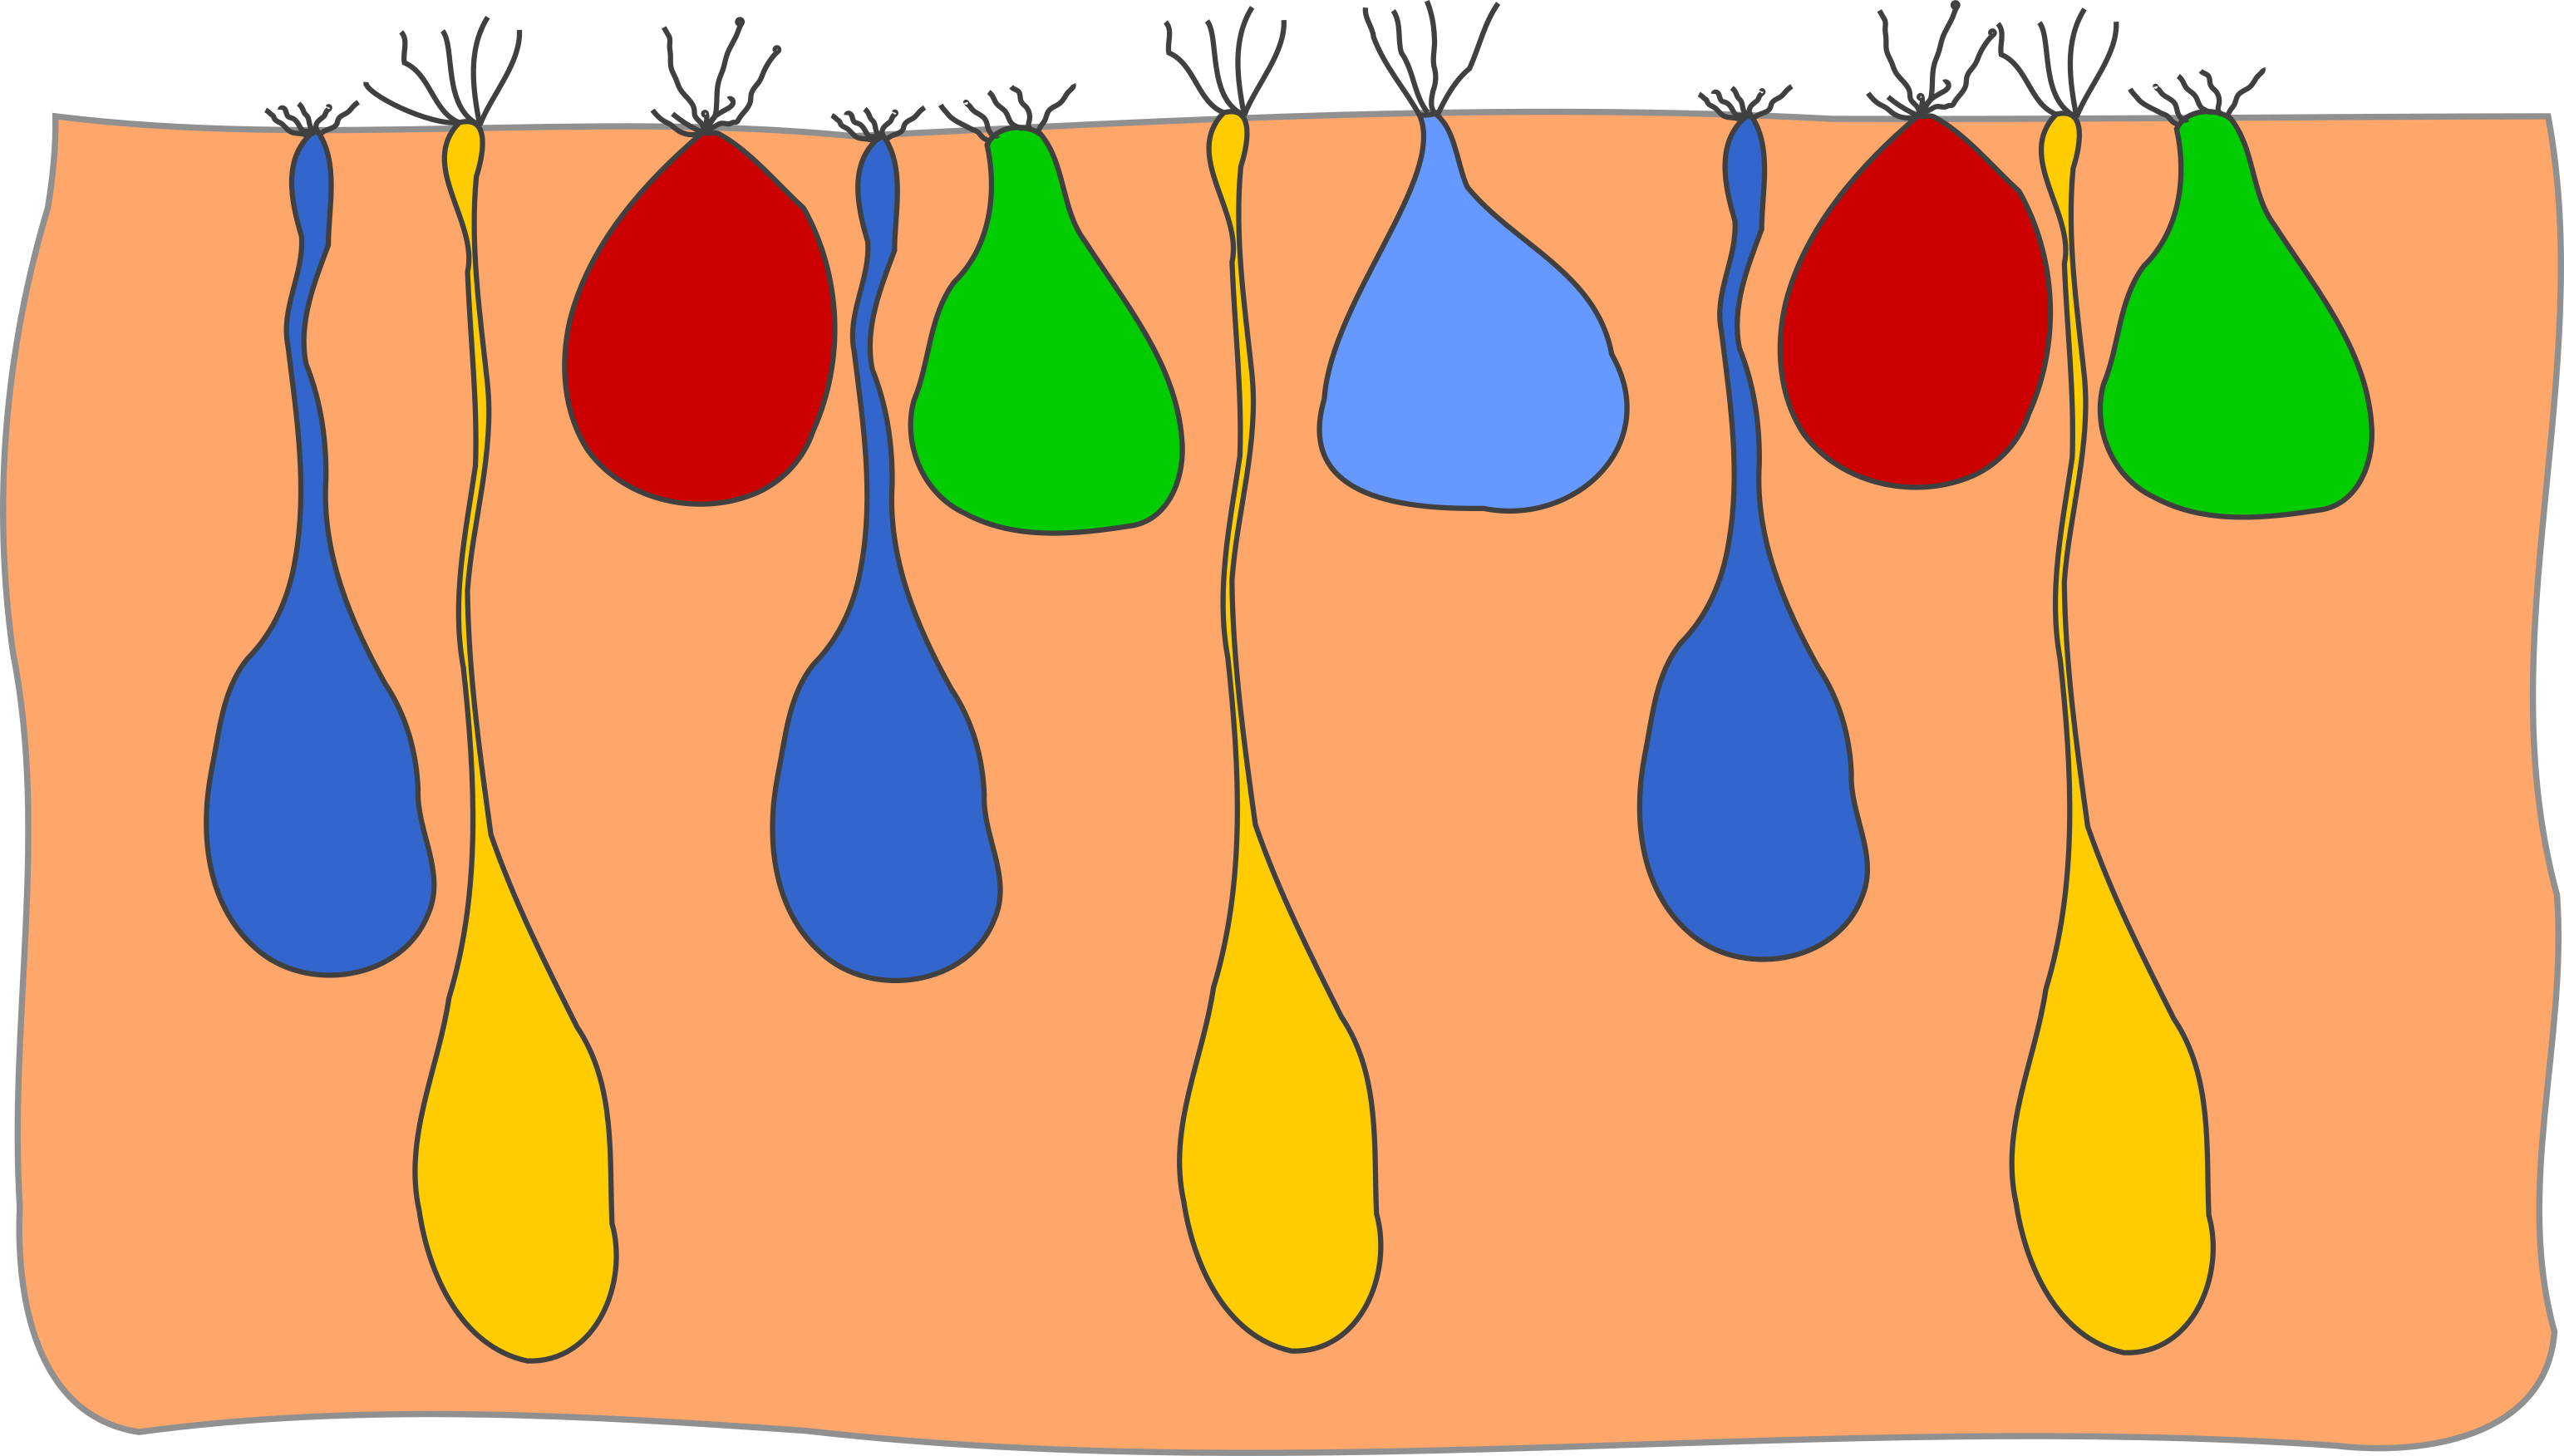
\includegraphics[width=10cm]{part_2/assets/olfactory_schematic_full.png}
      \caption{{\bf Schematic representation of the olfactory epithelium.} Ciliated neuron in yellow with round somata, slender dendrite, and cilia. Microvillous neuron in dark blue with microvilli at the surface. Crypt neuron in red with ovoid shape, microvilli, and cilia. Kappe neuron in green with microvilli. Pear-shaped neuron in light blue with cilia.}
      \label{olfactory_schematic_full}
    \end{figure}

    Receptor cells project directly into the olfactory bulb located in the brain, in turn sending signals to the telencephalon and diencephalon \cite{miyasaka2009olfactory}. The olfactory bulb in the teleost is a structure of four concentric layers: olfactory nerve layer (ONL), glomerular layer (GL), mitral cell layer (MCL), and internal cell layer (ICL). The olfactory information is transmitted by the receptor cells to the olfactory bulb \cite{nikonov2001electrophysiological} then in the forebrain \cite{nikonov2005beyond} as a topographical odor map. The olfactory bulb's neuronal connections have been particularly studied in the zebrafish \cite{hansen1998peripheral,kermen2013neural}, the olfactory bulb comprised approximately 20 000 neurons \cite{friedrich2009processing} and 140 glomeruli\cite{braubach2012distribution}. Each receptor cell expresses only one type of olfactory receptor \cite{serizawa2004one,barth1997noncoordinate,weth1996nested,sato2007hierarchical} except in a subpopulation of olfactory sensory neurons \cite{sato2007hierarchical}. Cells expressing the same receptor are projecting into the same olfactory bulb glomeruli \cite{sato2005mutually}. Glomeruli responding to similar odorants are grouped into domains within the olfactory bulb, forming chemotopic maps. Odorants can activate glomeruli outside their domain, leading to a fragmented map inside the olfactory bulb \cite{friedrich1998chemotopic}. Moreover, the odor encoding is hierarchized with first-order features encoded by large domains and second-order features by local activity patterns within the domain \cite{fuss2001odorant,korsching2001odor}.

    The olfactory bulb projects into two higher brain structures, the telencephalon (Dp and Vv) and the diencephalon (habenula, posterior tubercle, and hypothalamus). The neuronal activity evoked by olfactory cues in these areas is currently poorly understood \cite{kermen2013neural}.

    In the zebrafish \cite{hansen1993development,miyasaka2013functional}, the olfactory organ develops from the olfactory placodes at the 6-10 somites stage (about 15 hours post-fertilization) of the embryonic development. The olfactory cavity begins to appear at the 28-30 somites stage (31 hours post-fertilization). Approximately 50 hours post-fertilization, the olfactory epithelium and the receptor cells appear. When the embryo exits from the chorion at 4 days post-fertilization, the olfactory organ continues its morphological development, but the cytological organization remains largely unchanged. At 40 days post-fertilization, the bridge between the entrance nostril and the exit nostril is completely formed, separating the currents going out and coming in from the olfactory cavity. The addition of lamellae to the olfactory rosette continues throughout the life of the zebrafish.

    \subsection{Gustation}
    The gustatory organ of fish is composed of taste buds that are not localized in a single location but rather spread all over the body surface and directly contacting chemical substances. Taste bud histology has been studied for different fish \cite{kapoor1976gustatory,fishelson2004taste,reutter2000heterogeneity,reutter1991ultrastructure,reutter2012taste}, and they usually have an elongated and ovoid shape, see Figure~\ref{gustatory_schematic}. They sit on a small dermal papilla and extend throughout the epidermis' thickness protruding from the surface. The taste bud is constituted of a sensory (dark cells with microvilli and light cells with one large microvillus) and a non-sensory (Merkel‐like basal cells) epithelium. The apical ending of the sensory cells that protrude from the epithelium is called the receptor field and is covered with a mucous cap. The number of sensory cells in a taste bud varies considerably depending on the fish species, 2 200 on the zebrafish up to 1 000 000 in large \textit{Ictalurus nebulosus} \cite{kasumyan2019taste}.

    Taste buds are distributed all over the fish's body, especially in the mouth, on the lips, and the skin. Their distribution and concentration vary according to the species. Three different cranial nerves innervate them: facial (VII), glossopharyngeal (IX), and vagal (X). The facial nerve transmits information from the extra-oral taste buds; the glossopharyngeal nerve transmits information from inside the oral cavity; the vagal nerve transmits information from inside the oropharyngeal cavity. The taste system is anatomically divided into two distinct parts: nerves IX and X projecting into the brain's vagal lobe and nerve IV into the facial lobe. Connections to higher areas of the brain differ slightly from one species to another. It has been shown in \textit{Ictalurus nebulosus} \cite{atema1971structures} that these two systems have distinct roles in fish feeding behavior.

    \begin{figure}[h]
      \centering
      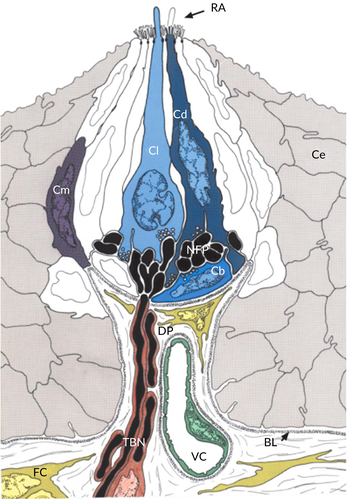
\includegraphics[width=8cm]{part_2/assets/gustatory_schematic.png}
      \caption{\textbf{Schematic drawing of a typical taste bud of teleosts from \cite{hansen2002taste}.} Dark cells (Cd), light cells (Cl) and Merkel‐like basal cells (Cb). Marginal cells (Cm). Ce epithelial cells. Dermal papilla (DP). (TBN) taste bud nerve. (BL) basal lamina. (RA) receptor area. (VC) capillary vessel.}
      \label{gustatory_schematic}
    \end{figure}

    In zebrafish \cite{ohkubo2005distribution}, the taste buds (approximately 2 200) are located on the lips, in the oropharyngeal cavity on the barbels, and on the head's ventral and dorsal side. Each taste bud contains 20 to 23 cells. Projections of the zebrafish gustatory system have been studied in detail \cite{yanez2017gustatory} and form a complex network that can be summarized graphically see Figure~\ref{gustatory_connection_schematic}.

    \begin{figure}[h]
      \centering
      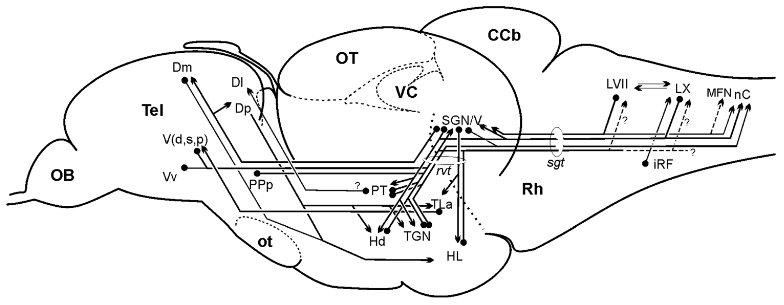
\includegraphics[width=10cm]{part_2/assets/gustatory_connection_schematic.png}
      \caption{\textbf{Gustatory system of the zebrafish}. Neuronal connections of the fish taste system reproduced from \cite{yanez2017gustatory}.}
      \label{gustatory_connection_schematic}
    \end{figure}

    The development of the gustatory organ has been studied in the zebrafish \cite{hansen2002taste}. The first taste buds appear at 3 or 4 days post-fertilization and are located on the lips and the gill arches. The taste buds in the mouth and oropharyngeal cavity appear 4 to 5 days post-fertilization. The taste buds on the head do not appear until 12 days post-fertilization, and it is not until the juvenile stage (30 to 40 days post-fertilization) that the barbels appear. Note that the appearance of the taste buds coincides with the appearance of feeding in the larvae.

    \subsection{Common chemical sense}
    Fish also have a third chemical sense called the common chemical sense. It consists of bipolar neurons called solitary chemosensory cells (SCCs) embedded in the epidermis. Their distribution and number vary greatly depending on the species. Therefore their study is difficult, and their function and neuronal connections are poorly understood.

    In the zebrafish \cite{kotrschal1997ontogeny}, SCCs have been described as a set of 2-7 villi of 0.5 to 1 $\mu m$ length emerging from the cell body at embryo and larval stage.  In adults, SCCs possess a single villus of $3\mu m$ length.

    The first SCCs appear at 3 days post-fertilization. Their density increases until 25 days, where their number stabilizes at $1.10^6$ per $mm^2$ with 2 to 5 times more SCCs on the zebrafish's head than on its body.


  \section{Behavioral studies}
    \subsection{Behavior}
    The olfaction and gustation have been shown to mediate several fish behaviors. It is not easy to distinguish the contribution of each sense in the observed behavior. Moreover, this contribution seems to be dependent on fish species.

    A well known and impressive behavior encountered in many fish species is the homing migration. A typical example is salmons that perform three migratory phases throughout their life. One of them, the upstream migration from the ocean to their home stream, has been shown to rely on an olfaction imprinting \cite{stabell1992olfactory,hasler1983olfactory}. Little is known about the imprinting mechanism, but experiments suggest that it relies on a mixture of odors perceived during the juvenile stage in the fish's home stream.

    Feeding is one of the most important behaviors. It relies on several senses for food detection and selection \cite{pavlov1990sensory}. A stereotyped behavioral sequence was shown to exist in many species \cite{atema1980chemical} consisting in a step of arousal mainly mediated by olfaction \cite{bateson1890sense}, then a step of localization of the food mediated by chemical and visual cues. The last step of ingestion is triggered primarily by the gustation \cite{atema1980chemical}. The impact of each sensory modality varies significantly with the species. For example, the yellow bullhead has the entire feeding sequence mediated by taste, whereas ictalurid catfish prey detection was abolished when olfaction was blocked. The chemical substances that attract fish depend on the species \cite{atema1980chemical}, and response to a mixture is higher than isolated compounds in general.

    Olfaction \cite{tavolga1956visual} as well as the gustatory system \cite{de1983influence} has been shown to play an essential role in reproduction. Non-anosmic males exposed to water taken from a tank with a gravid female developed courtship behaviors, except for some species like the three-spined stickleback where the gustation can replace the olfaction. Complete courtship repertoire necessitated the presence of other sensory cues.

    Fright reaction occurred when a fish perceived an alarm substance secreted by a conspecific. This reaction differs between species and involves seeking cover, rapid swimming, or freezing. It is accepted to be mediated by olfaction \cite{frisch1942schreckstoff,speedie2008alarm,doving2009alarm}, but other sensory cues are not ruled out.

    Most of the works done on the zebrafish chemically induced behaviors focus on developing the model for pharmacological safety screening \cite{cassar2019use}, drugs addiction \cite{klee2012zebrafish}, and ecology \cite{dai2014zebrafish}, enabling a low cost and genetically manipulable model. Behavioral studies of the chemical perception of zebrafish, adults, or at the larval stage have been done through various experimental assays that will be presented in the following sections.

    \subsection{Conditioned place preference}
    The conditional place preference (CPP) experiment is a type of Pavlovian conditioning. Pavlovian conditioning consists of associating a conditioned stimulus (generally neutral) with an unconditioned stimulus. After learning, the animal exhibits a conditioned response to the conditioned stimulus when presented alone. The most classic example is associating a bell's sound (conditioned stimulus) to the release of a food smell (unconditioned stimulus). After learning, the animal can respond to the bell's sound alone, as demonstrated by Ivan Pavlov on dogs \cite{pavlov1903experimental}.

    This approach was applied to test the response to various chemical stimuli in adult zebrafish \cite{mathur2011conditioned}. The experiment follows a classical 3-step design. The first step is to evaluate the fish's base-line preference. The animal is placed in an aquarium with two or three distinct areas differentiate by walls' pattern and color, see Figure~\ref{cpp_schematic}. The fish is tested to find out which side it naturally prefers. In this experiment, the distinctive walls' pattern and color play the role of the conditioned stimulus. The second step is the conditioning phase. The fish is restrained to its least preferred area, and the substance to be tested injected into the water (unconditioned stimuli). The last step consists of repeating the first step to assess the change in preference of the animal.

    Several chemical substances have been tested using this method \cite{blaser2014experiments,collier2013utility,tzschentke2007review}. Notably, a strong and robust cocaine-induced CPP response in WT zebrafish was shown \cite{darland2001behavioral}, with $85\%$ of the fish changing preference to a cocaine concentration of $10mg.L^{-1}$ and lower and higher concentrations resulting in a lower response. A positive response of adult zebrafish to a single ethanol exposure was shown \cite{mathur2011preference} in a similar experimental setup. It should be noted that this is also the first study to use an automated tracking system to calculate animal preference. Zebrafish showed a positive response for D-amphetamine \cite{ninkovic2006genetic, ninkovic2006zebrafish}, salvinorin A \cite{braida2007hallucinatory}, cocaine \cite{braida2007hallucinatory}, spiradoline \cite{braida2007hallucinatory}, nicotine \cite{kedikian2013behavioral} and ethanol \cite{kedikian2013behavioral}.

    We see that CPP has been used extensively to study the response to chemical stimuli in zebrafish. There is a strong emphasis on products that cause addictive pathologies in humans. Nevertheless, this protocol has several limitations, the most important being that it involves several systems of perception as well as memory. During the conditioning phase, the learning is based on the visual perception of the environment (pattern on the aquarium walls), the chemical perception of the tested compound, the association of the two stimuli coming from different sensory organs, and the memorization of these perceptions. Secondly, the time window to perform the experiment (minimum two days) and the difficulty to automate it is a hindrance to use the CPP to study the effect of many chemicals in a high-throughput manner. Furthermore, this protocol is too complex to be used with larval zebrafish and coupled with neuronal imaging.

    \begin{figure}[h]
      \centering
      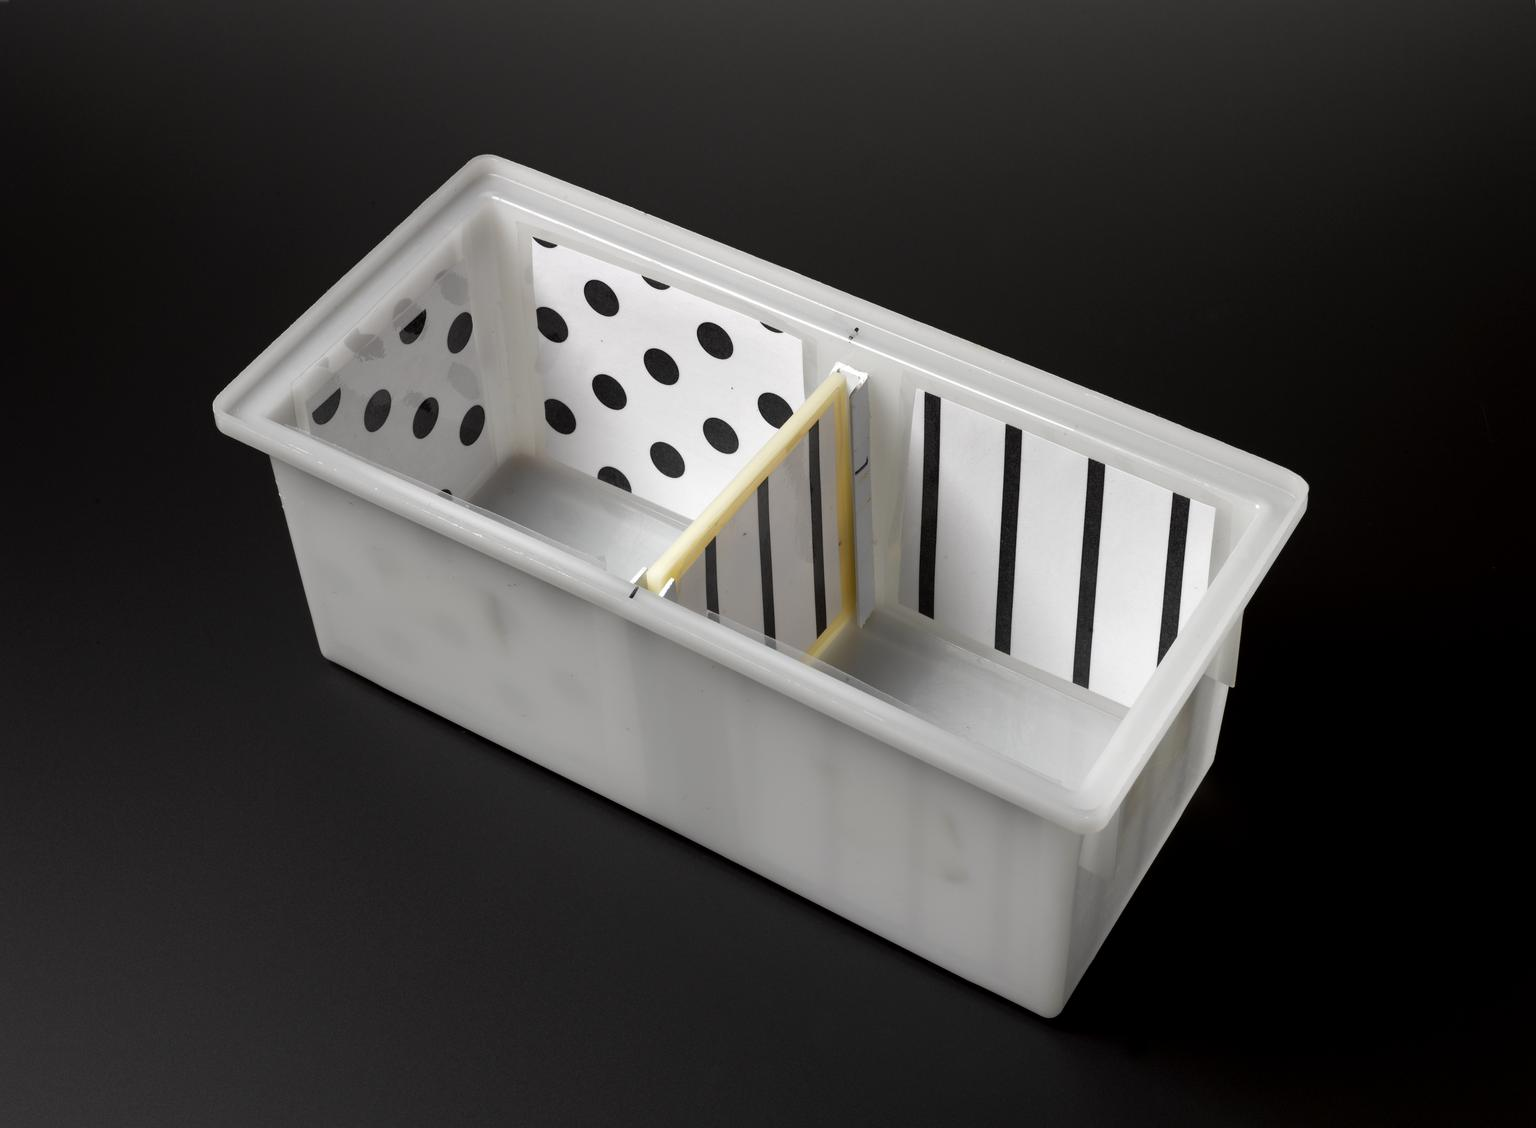
\includegraphics[width=0.8\textwidth]{part_2/assets/cpp.jpg}
      \caption{\textbf{Conditioned place preference apparatus}.  CPP setup for zebrafish reproduced from Brennan Caroline, Queen Mary University of London. The middle wall is removed for the first and third step of the CPP.}
      \label{cpp_schematic}
    \end{figure}

    \subsection{Multi well-plate}
    A widely used experimental apparatus to assess chemical compounds' effect on zebrafish larvae and embryos is the well-plate device \cite{rennekamp201515}. One or more larvae is placed in each well in a bath of a chemical. Larvae are then recorded swimming in the chemical compound, and the kinematic parameters of the animal are extracted. In the case of embryos, development is monitored after exposure. The advantage of this technique is that it requires only a single experimental apparatus. It quickly produces a large amount of data with up to 48 wells per plate. Software already exist to extract automatically relevant behavior parameters from video recordings \cite{zhou2014quantification}.

    With this kind of assay, many chemical compounds have been tested \cite{sallinen2009mptp,rihel2010zebrafish,kokel2010rapid}, as well as seizure liability \cite{winter2008validation}, and several behaviors \cite{farrell2011evaluation, shen2020rapid,schnorr2012measuring,pelkowski2011novel}.

    The well-plate device allows for an easy and automatic high-throughput screening of chemicals. Turnkey commercial solutions like the Zebrabox from ViewPoint exist, and custom setups are relatively easy to build. However, this system suffers limitations like the fact that one can not assess the fish preference. Precisely controlled exposure, or repeated exposure through cycles of exposition/flushing, are not available. Therefore this system is not adapted to investigate fish's chemical preference and chemical-driven navigation.

    \begin{figure}[h]
      \centering
      \includegraphics[width=0.4\textwidth]{part_2/assets/well.png}
      \caption{\textbf{A Zebrabox from Viewpoint}.  Zebrabox, the most used solution for well-plates experiments.}
      \label{zebrabox}
    \end{figure}

    \subsection{Direct introduction}
    Some authors have tried to quantify chemically induced behavior by introducing a chemical compound directly into the tank and looking at the percentage of time spent close to the source. Notably, an attraction concentration-dependent to adenosine and ATP for adult zebrafish\cite{wakisaka2017adenosine} and to GCDA and nicotine for zebrafish larval \cite{krishnan2014right} was shown. A strong aversion to cadaverine, an odor associated with decomposing bodies, was shown using a tank with a single compartment or a tank with two compartments and an intermediate zone where the fish can changes compartment \cite{hussain2013high}, see Figure~\ref{diffusion_setup}.

    Very easy to implement, these types of experimental devices lack control in the concentration perceived by the animal. Diffusion and advection are neglected in the experiment, and the concentration is poorly known and not reproducible. Moreover, these setups exclude the realization of long experiments due to the homogenization of the product.

    \begin{figure}[h]
      \centering
      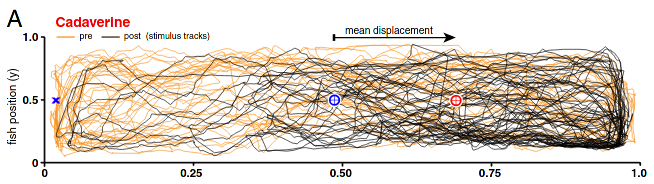
\includegraphics[width=1\textwidth]{part_2/assets/diffusion.png}
      \caption{\textbf{Diffusion setups from \cite{hussain2013high}}. \textbf{A.} One channel diffusion setup, blue cross: chemical introduction point.}
      \label{diffusion_setup}
    \end{figure}

    \subsection{Flow}
    Another type of device that allows the product's concentration inside the tank to be quickly changed was used on adult zebrafish \cite{kermen2020stimulus}, see Figure~\ref{flow_1_setup}. Like in the multi-well experiment, chemically induced behavior changes were monitored by the animal's kinematic parameters.

    Several food odors were shown to produce a significant increase in speed and number of bursts; social odors from conspecific produced a similar response; alert odors result in a dive to the bottom of the tank and an increase in frozen time; decomposition odors result in more turns. The critical points noted with this device is the inter-and intra-experimental variability. The authors showed that less than a third of the odors used in the study produce reproducible results between trials of the same individual. Some odors such as cadaverine, blood, skin, and food odors resulted in inconsistent responses for the same individual. Most odors produce poorly reproducible results for different fish.

    \begin{figure}[h]
      \centering
      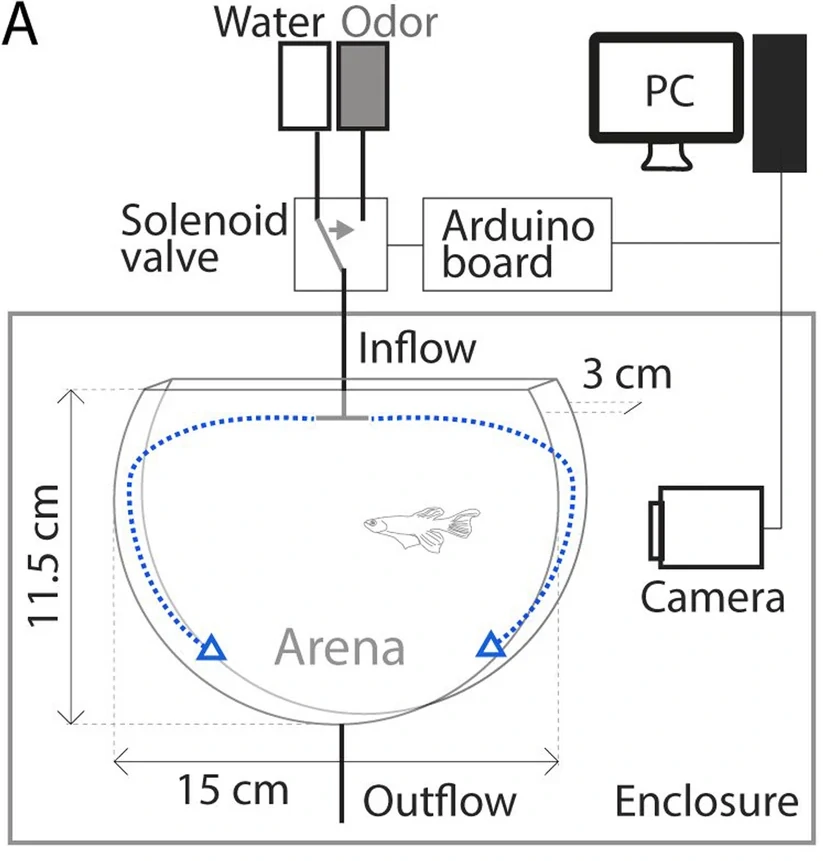
\includegraphics[width=0.5\textwidth]{part_2/assets/flow_1.png}
      \caption{\textbf{Flow setup from \cite{kermen2020stimulus}.}}
      \label{flow_1_setup}
    \end{figure}

    This setup novelty is to allow adult animals to evolve realistically in a 3D environment and to have a better knowledge of the concentration perceived by the animal than in a diffusion setup. Therefore, direct preference assessment is not accessible, and comparisons with existing quasi-2D setups like the well-plate are difficult.

    A more controlled setup to study chemical preference in fish is the underflow device. The first mention of this type of device dates back to 2013 \cite{readman2013fish}. In this setup, the tank is separated into two distinct compartments using a laminar flow, see Figure~\ref{flow_0_setup}. The animal can then choose between the two compartments during the experiment without any constraint, and the experimenter can put a chemical to test on one side. The interface between the two compartments self-heal with a characteristic time depending on the flow velocity. The time spent on each side, the number of interface crosses, and the animal's kinematic parameters are extracted from video recordings to assess the fish's preference.

    Several psychoactive substances have been tested on adult zebrafish \cite{abreu2016acute, abreu2016behavioral} and showed attraction by diazepam, fluoxetine, risperidone, and buspirone; neutral response to ethanol and clonazepam; an aversion to acid pH, two food odor extracts, and conditioned water took from a tank with chemically and physically stressed fish.

    This setup has several advantages. The product's concentration is perfectly known because the diffusion and advection are mitigated and controlled by the flow. The fish's preference can be directly measured as the fish can choose freely to go inside or outside the product. Long experiments can be performed with this setup, and product delivery precisely controlled in time. However, some disadvantages remain, like the absence of a standardized or turnkey setup and the volume of water and chemicals required that can be high.

    \begin{figure}[h]
      \centering
      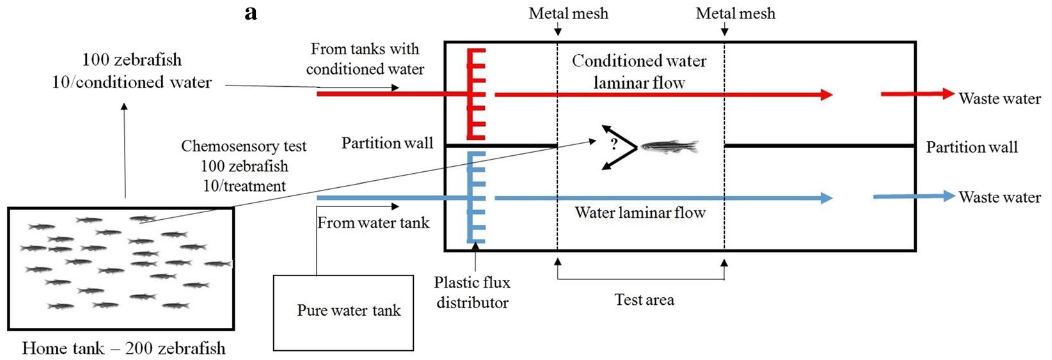
\includegraphics[width=1\textwidth]{part_2/assets/flow_0.png}
      \caption{\textbf{Flow setups from \cite{abreu2016behavioral}} The flow is separating the tank in two lines (left-right).}
      \label{flow_0_setup}
    \end{figure}

    From this overview of the scientific literature, we see that the study of chemical perception and behavioral response to chemical stimuli is not standardized. Direct comparisons between studies carried out in various independent laboratories are not easily possible. In this context, we have developed Dual, an open-source, easy to replicate, low cost, do it yourself, and scalable experimental setup. Using the underflow principle, Dual allows studying chemical preferences in larvae and juvenile zebrafish in a standardized, high-throughput, and comparable way.

\chapter{Experimental setups}
  To study the young zebrafish chemical perception, we build two complementary setups: one to screen products, the other to recreate more natural flows, and studies the chemically-driven navigation.

  \section{Dual}
  The design and implementation of experimental setups that are high-throughput, bias-free, and scalable are essential to behavior characterization. We present Dual, a high-throughput experimental setup that is easy to build, scalable, and costs less than 2 000 euros.

  \subsection{Overview}
  Dual is an underflow system built on the same principle as \cite{readman2013fish}. It consists of creating two compartments in a tank through a laminar flow without any physical separation. As we have seen previously, this system allows a rigorous knowledge of the compound's concentration to which the animal is subjected. Diffusion and advection due to the water movements caused by the fish are avoided. The interface between the two compartments is well defined and self-healing when disturbed, with a characteristic time depending on the flow rate.

  To create the laminar flow, Dual uses a system of four syringes, coupled two by two: when two syringes push, two syringes pull, see Figure~\ref{dual_mechanical}. The syringes are connected to the inputs and outputs of a millifluidic chip and generate a laminar flow with constant volume by having two syringes injecting at one side and two aspirating at the other side. The fish is placed inside the millifluidic chip, see Figure~\ref{dual_chip_visu}. Thanks to a computer-controlled manifold composed of six microvalves, each syringe can be filled independently. One can then build an experimental protocol by stacking several filling and injection cycles and choosing what to fill the syringes with.

  To assess fish preference, one can first create a cycle with water on the two sides as habituation and control. Then add a cycle with a chemical on one side and water on the other side to study the fish preference. Another example is to fill the two sides with a chemical for a given amount of time and then clean the system with water on the two sides, reproducing the type of experiment performed with the multi well-plate device. A large variety of experiments can be designed with none or few setup modifications.

  Dual is a custom-built system using several components stemming from the makers' community (Openbuilds, Markerbeam, Arduino), which allows great flexibility in the conception and fast iteration to adapt the project if necessary. All the components, blueprints, and other CAD files needed to build and assemble Dual are freely available. Dual can be built at a low-cost (see the bill of materials Appendix~\ref{bom}) without prior knowledge of mechanics or electronics. The tools necessary for realizing Dual can be found in a FabLab and necessitate little formation.

    \begin{figure}[h]
      \centering
      \includegraphics[width=0.80\textwidth]{part_2/assets/dual_photo.jpeg}
      \caption{\textbf{Four Dual setups in parallel.}}
      \label{dual_photo}
    \end{figure}

  \subsection{Construction}
  For the construction, Dual can be separated into five main parts. The mechanical system comprised the static structures, the motor, and moving parts. The millifluidic system is constituted of the millifluidic chip, the microvalves, the syringes, and connecting tubes. A camera, lens, infrared filters, and LEDs form the imaging system. The electronic system is a custom PCB controlling the motor and the microvalves. Finally, a software that controls all the setup automatically.

  \subsubsection{Mechanical}
  Dual's central mechanical part is a motorized syringe pump that creates the laminar flow. It is built around the V-Slot Linear Actuator from OpenBuilds fixed on a structure build using OpenBuilds linear rails and 3D printed fixations. A stepper motor with a gearbox (85:1) drives the actuator, and two microswitches limit the range of motion, see Figure~\ref{dual_mechanical}.

    \begin{figure}[h!]
      \centering
      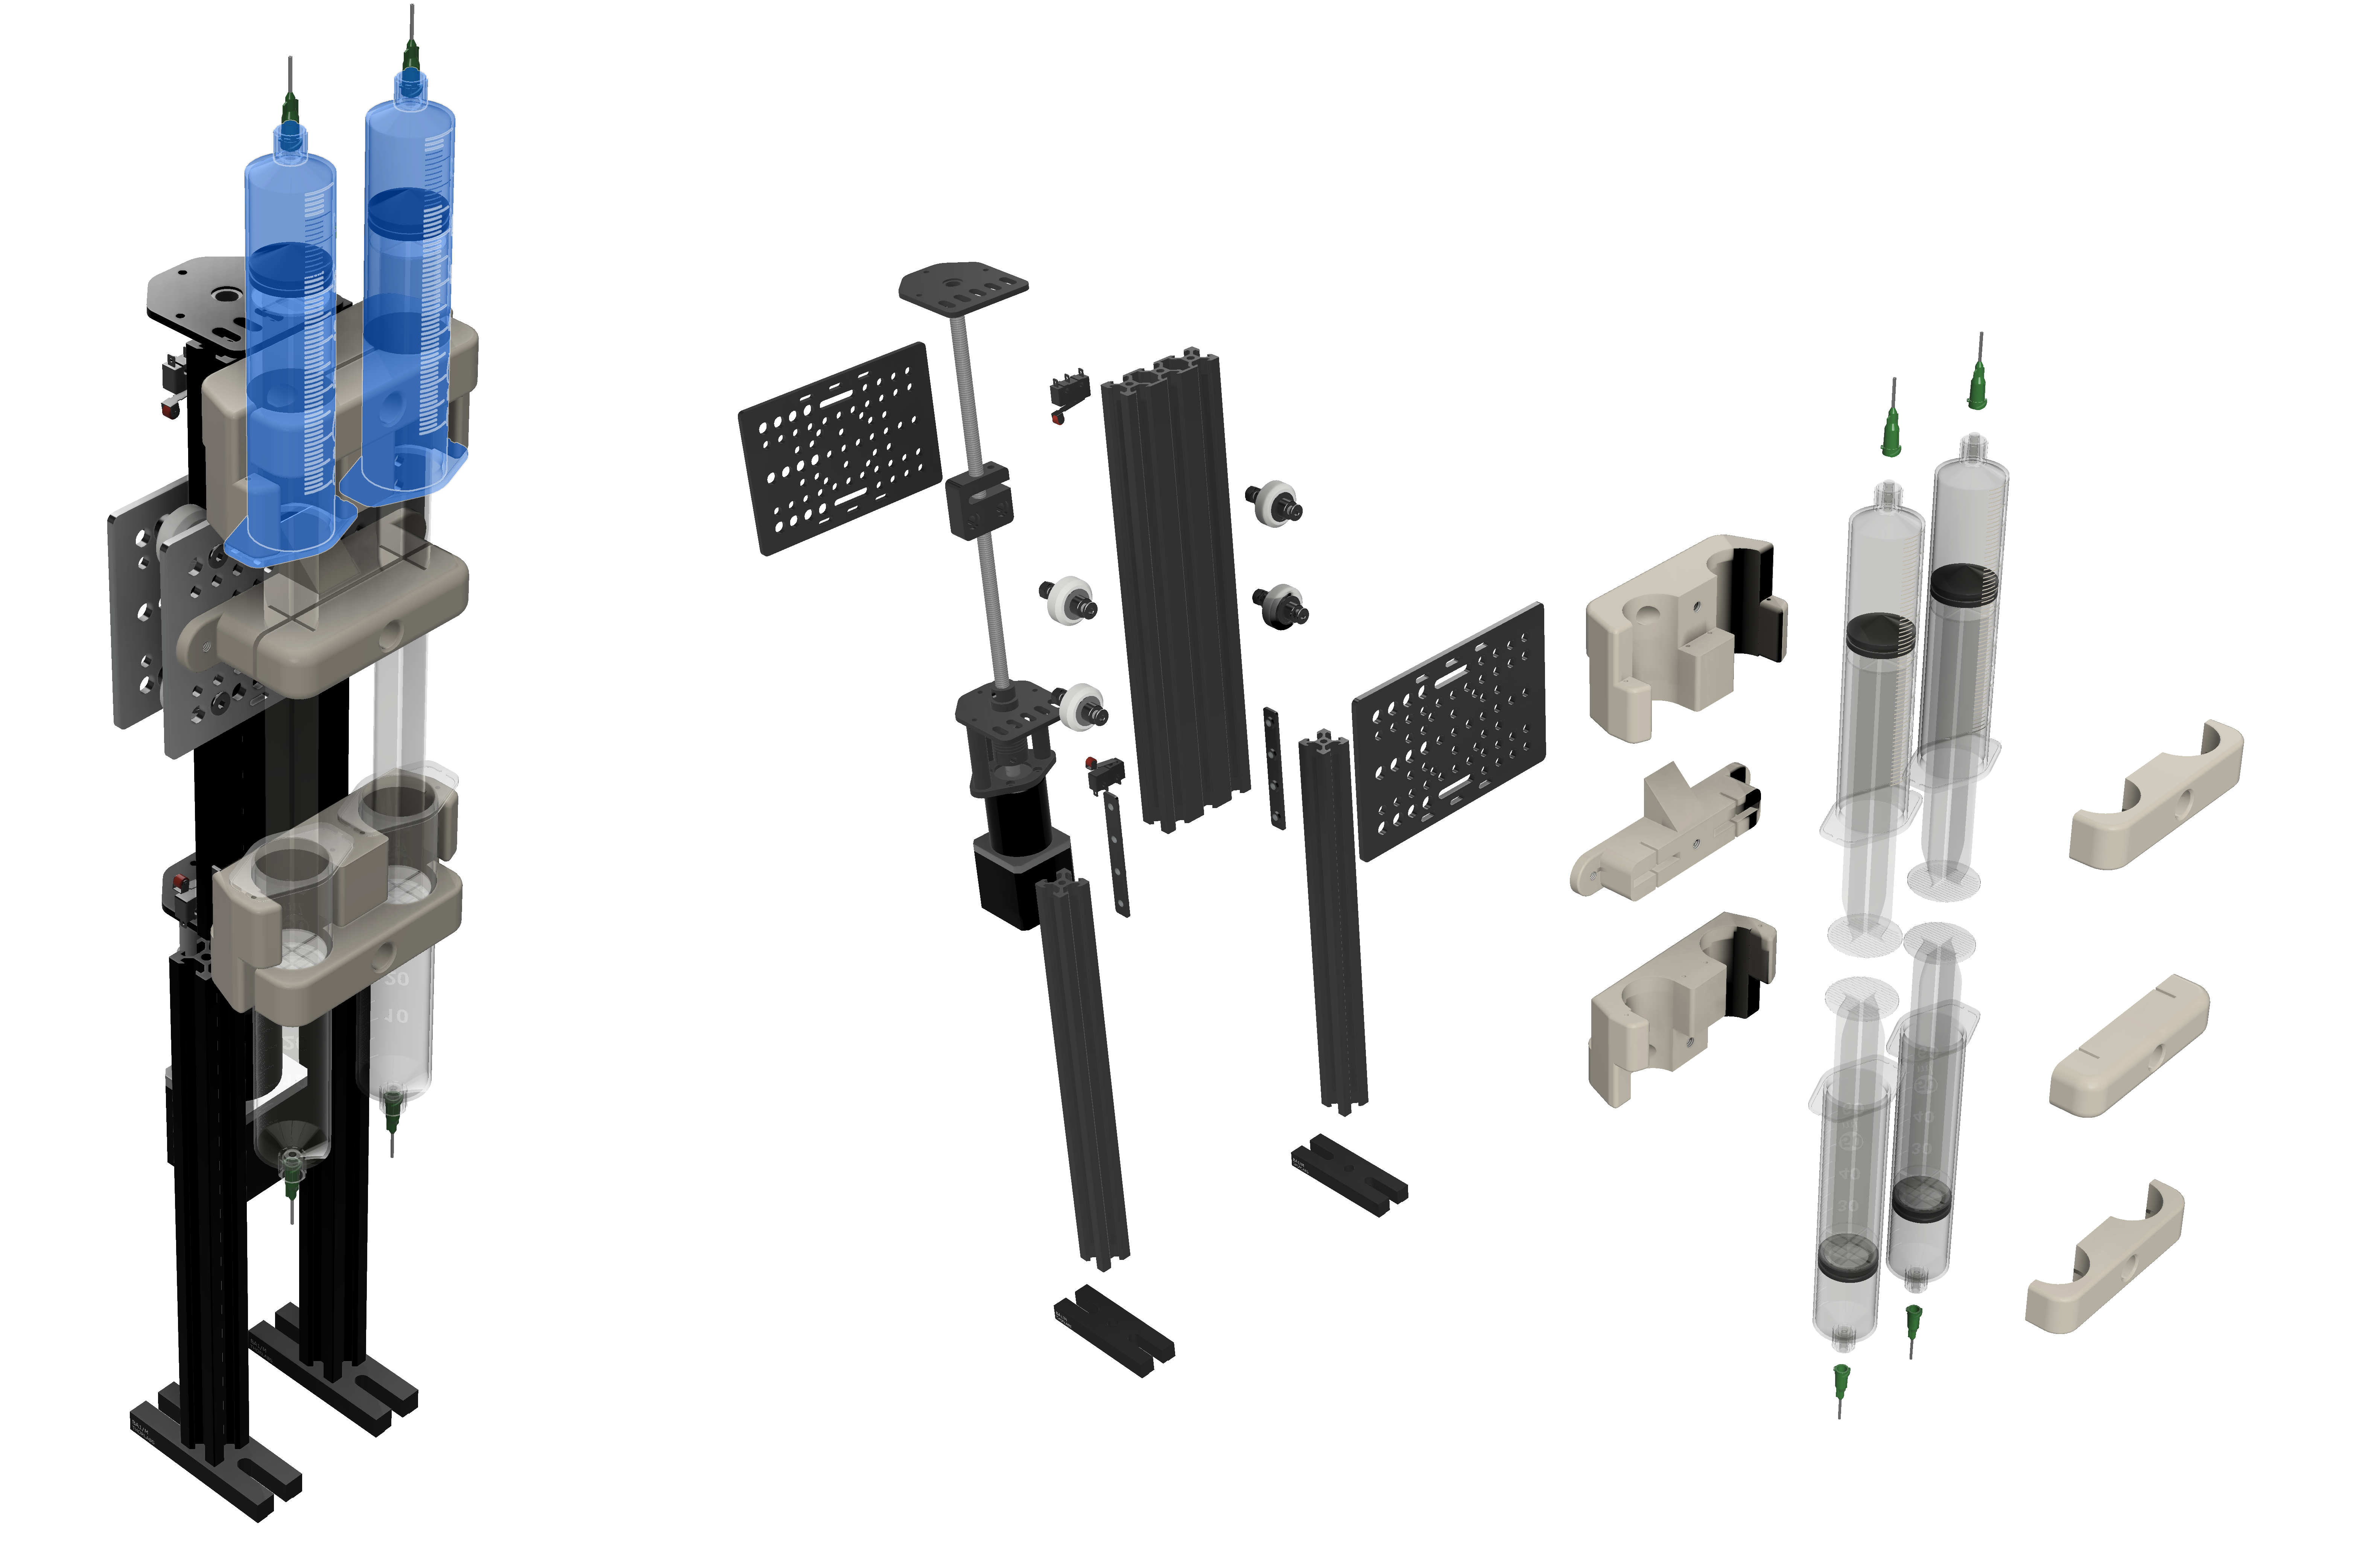
\includegraphics[width=0.95\textwidth]{part_2/assets/pull_push.png}
      \caption{\textbf{Dual mechanical structure} Dual custom pull-push syringe.}
      \label{dual_mechanical}
    \end{figure}

  It is crucial to isolate the animal from the exterior environment and of any light sources. A box that contains the millifluidic chip and lighting system is constructed using MakerBeam rails and medium-density fibreboard sheets. A PMMA infrared transparent sheet is placed on the removable top panel to record the experiment while blocking visible light. The box contains, see Figure~\ref{dual_box}, two LEDs for visible and infrared light, a diffuser for homogeneous lighting, and a support to fix the millifluidic chip.

  A structure to maintain the camera on top of the box and secure the Raspberry and the power alimentation is built using OpenBuilds rails. It is better to build Dual on top of an optical breadboard to facilitate fixation and enhanced stability. All these elements need to be fixed firmly and leveled to avoid any bias that could disturb the animal during the experiment.

    \begin{figure}[h!]
      \centering
      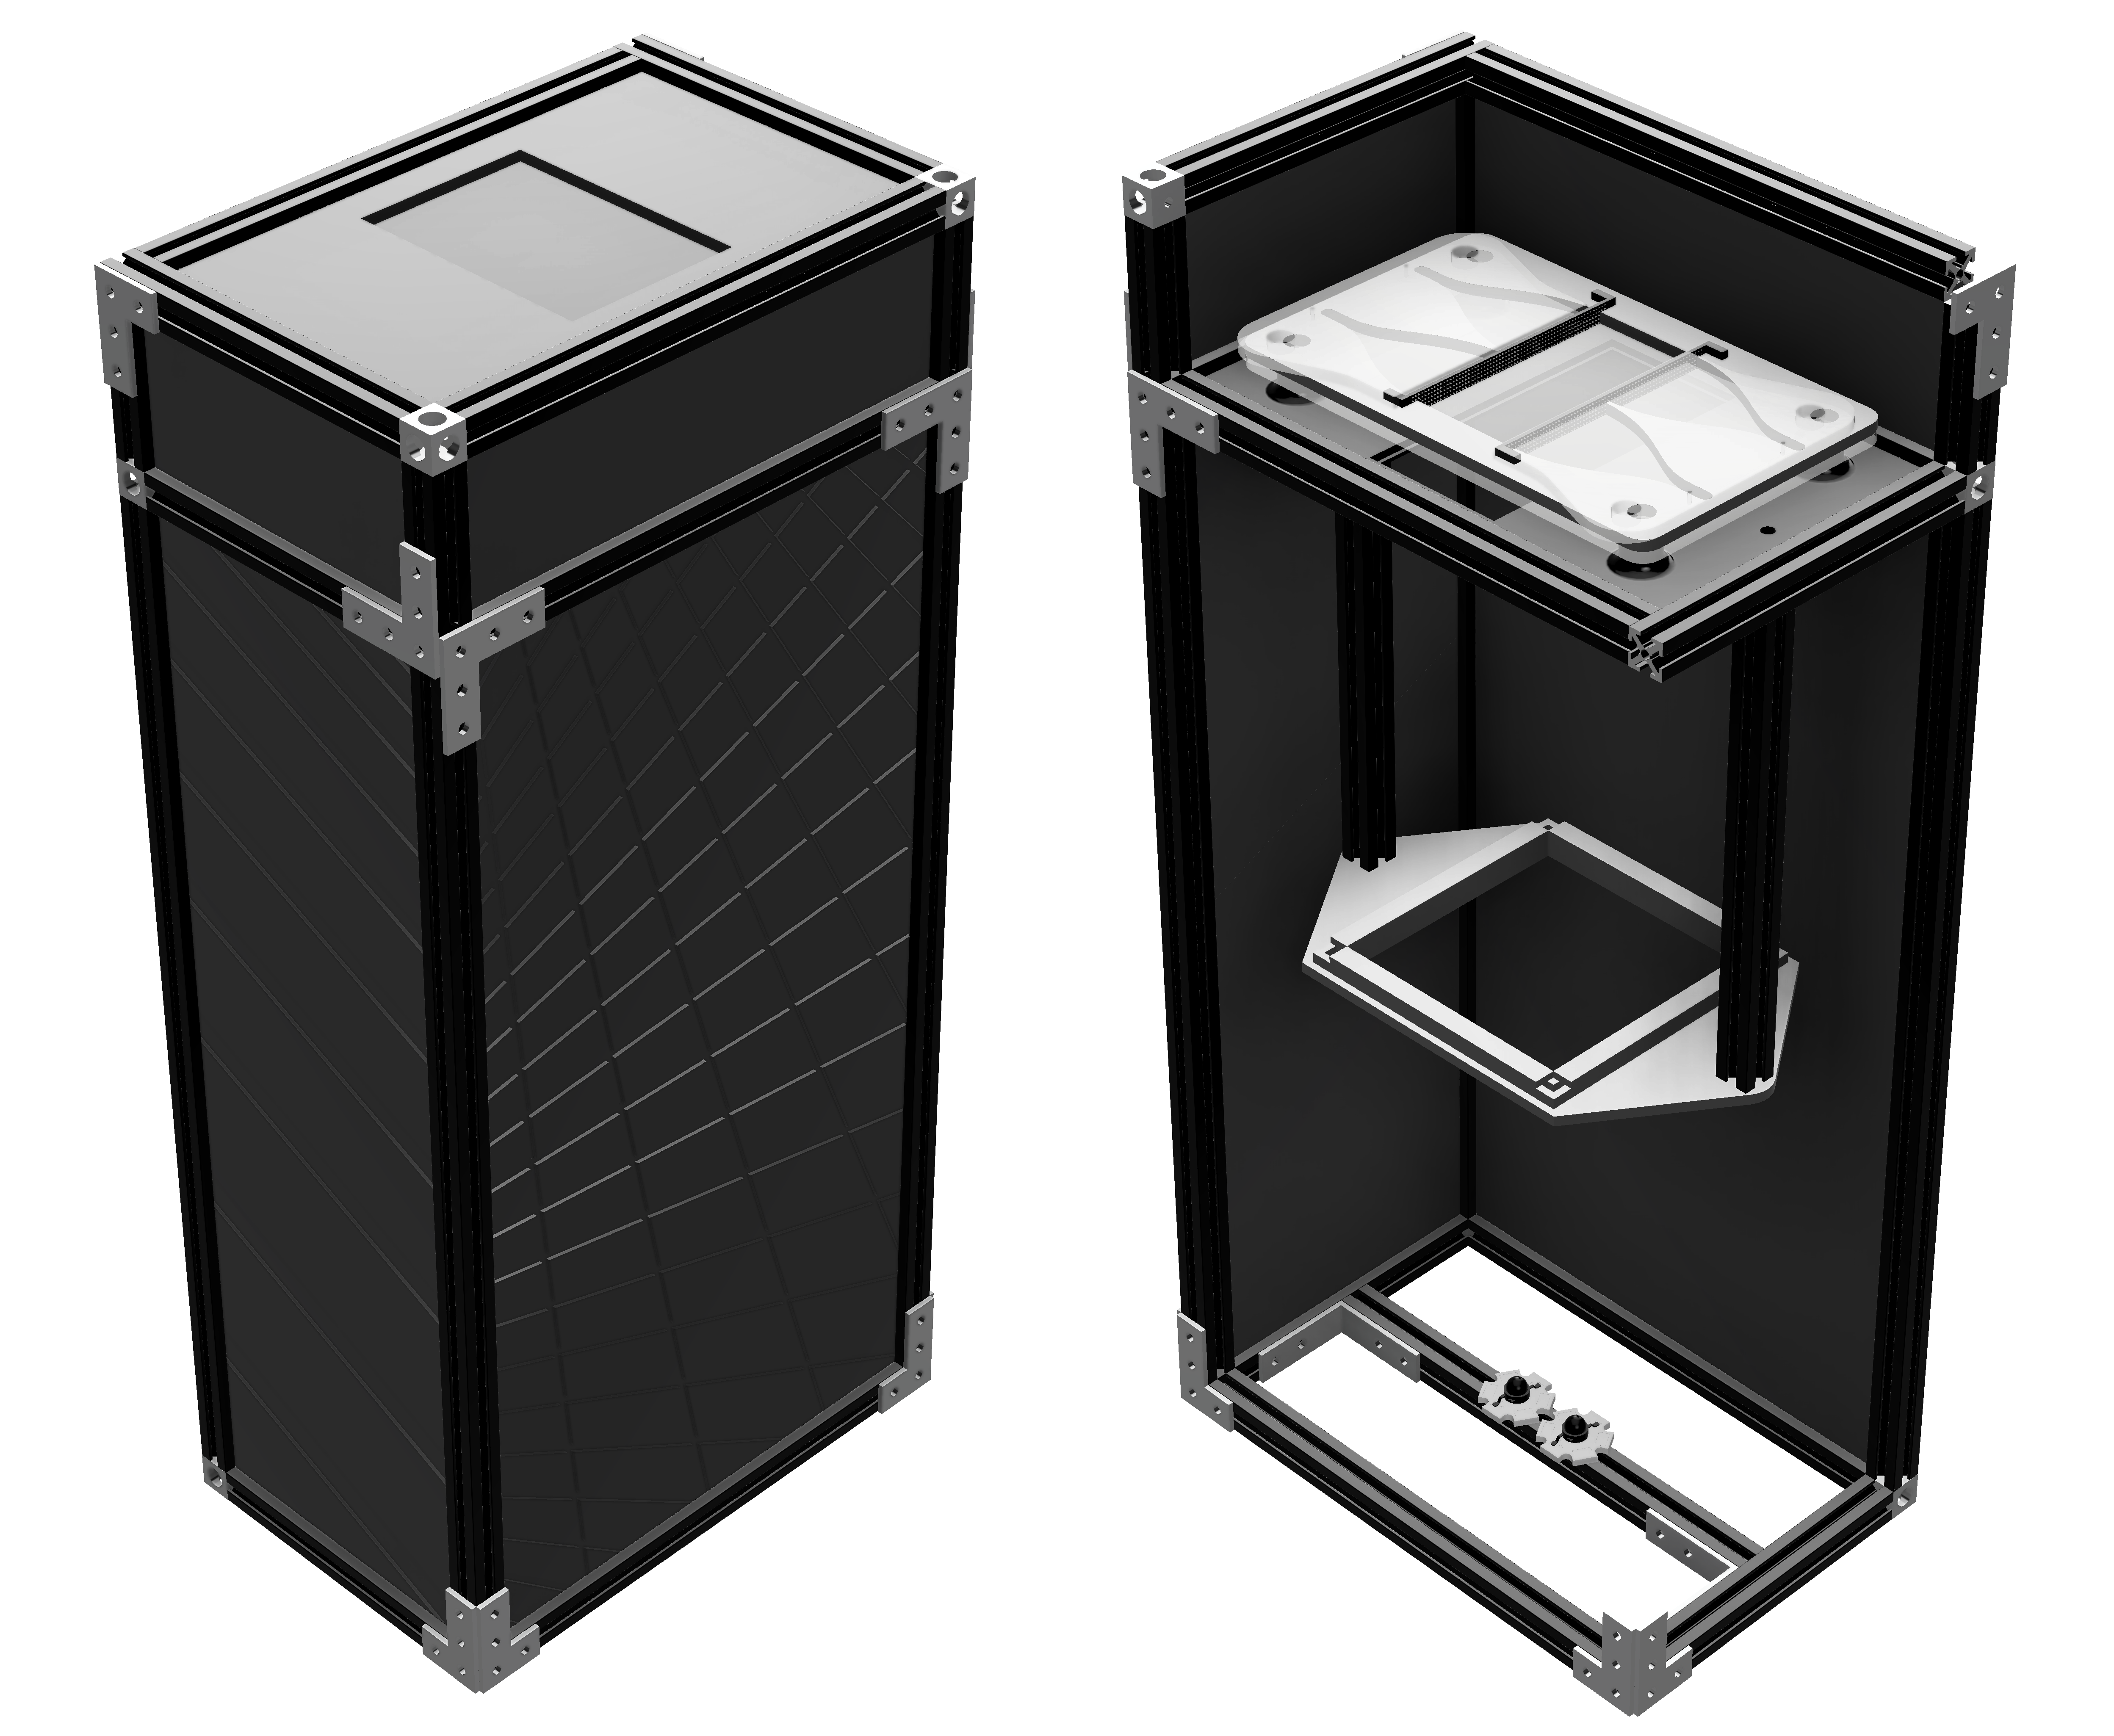
\includegraphics[width=0.75\textwidth]{part_2/assets/box.png}
      \caption{\textbf{Box} The box isolates the animal from the exterior.}
      \label{dual_box}
    \end{figure}

  \subsubsection{Millifluidic}
  The millifluidic chip that serves as a tank for the fish, see Figure~\ref{dual_chip_visu}, is laser cut in PMMA plastic that is transparent and presents excellent optic properties. The different parts are bonded using acetic acid \cite{trinh2019clog}. The fish is restrained in the center by 3D printed and micro-machined nets, and profiled inputs and outputs allow a laminar flow.

    \begin{figure}[h!]
      \centering
      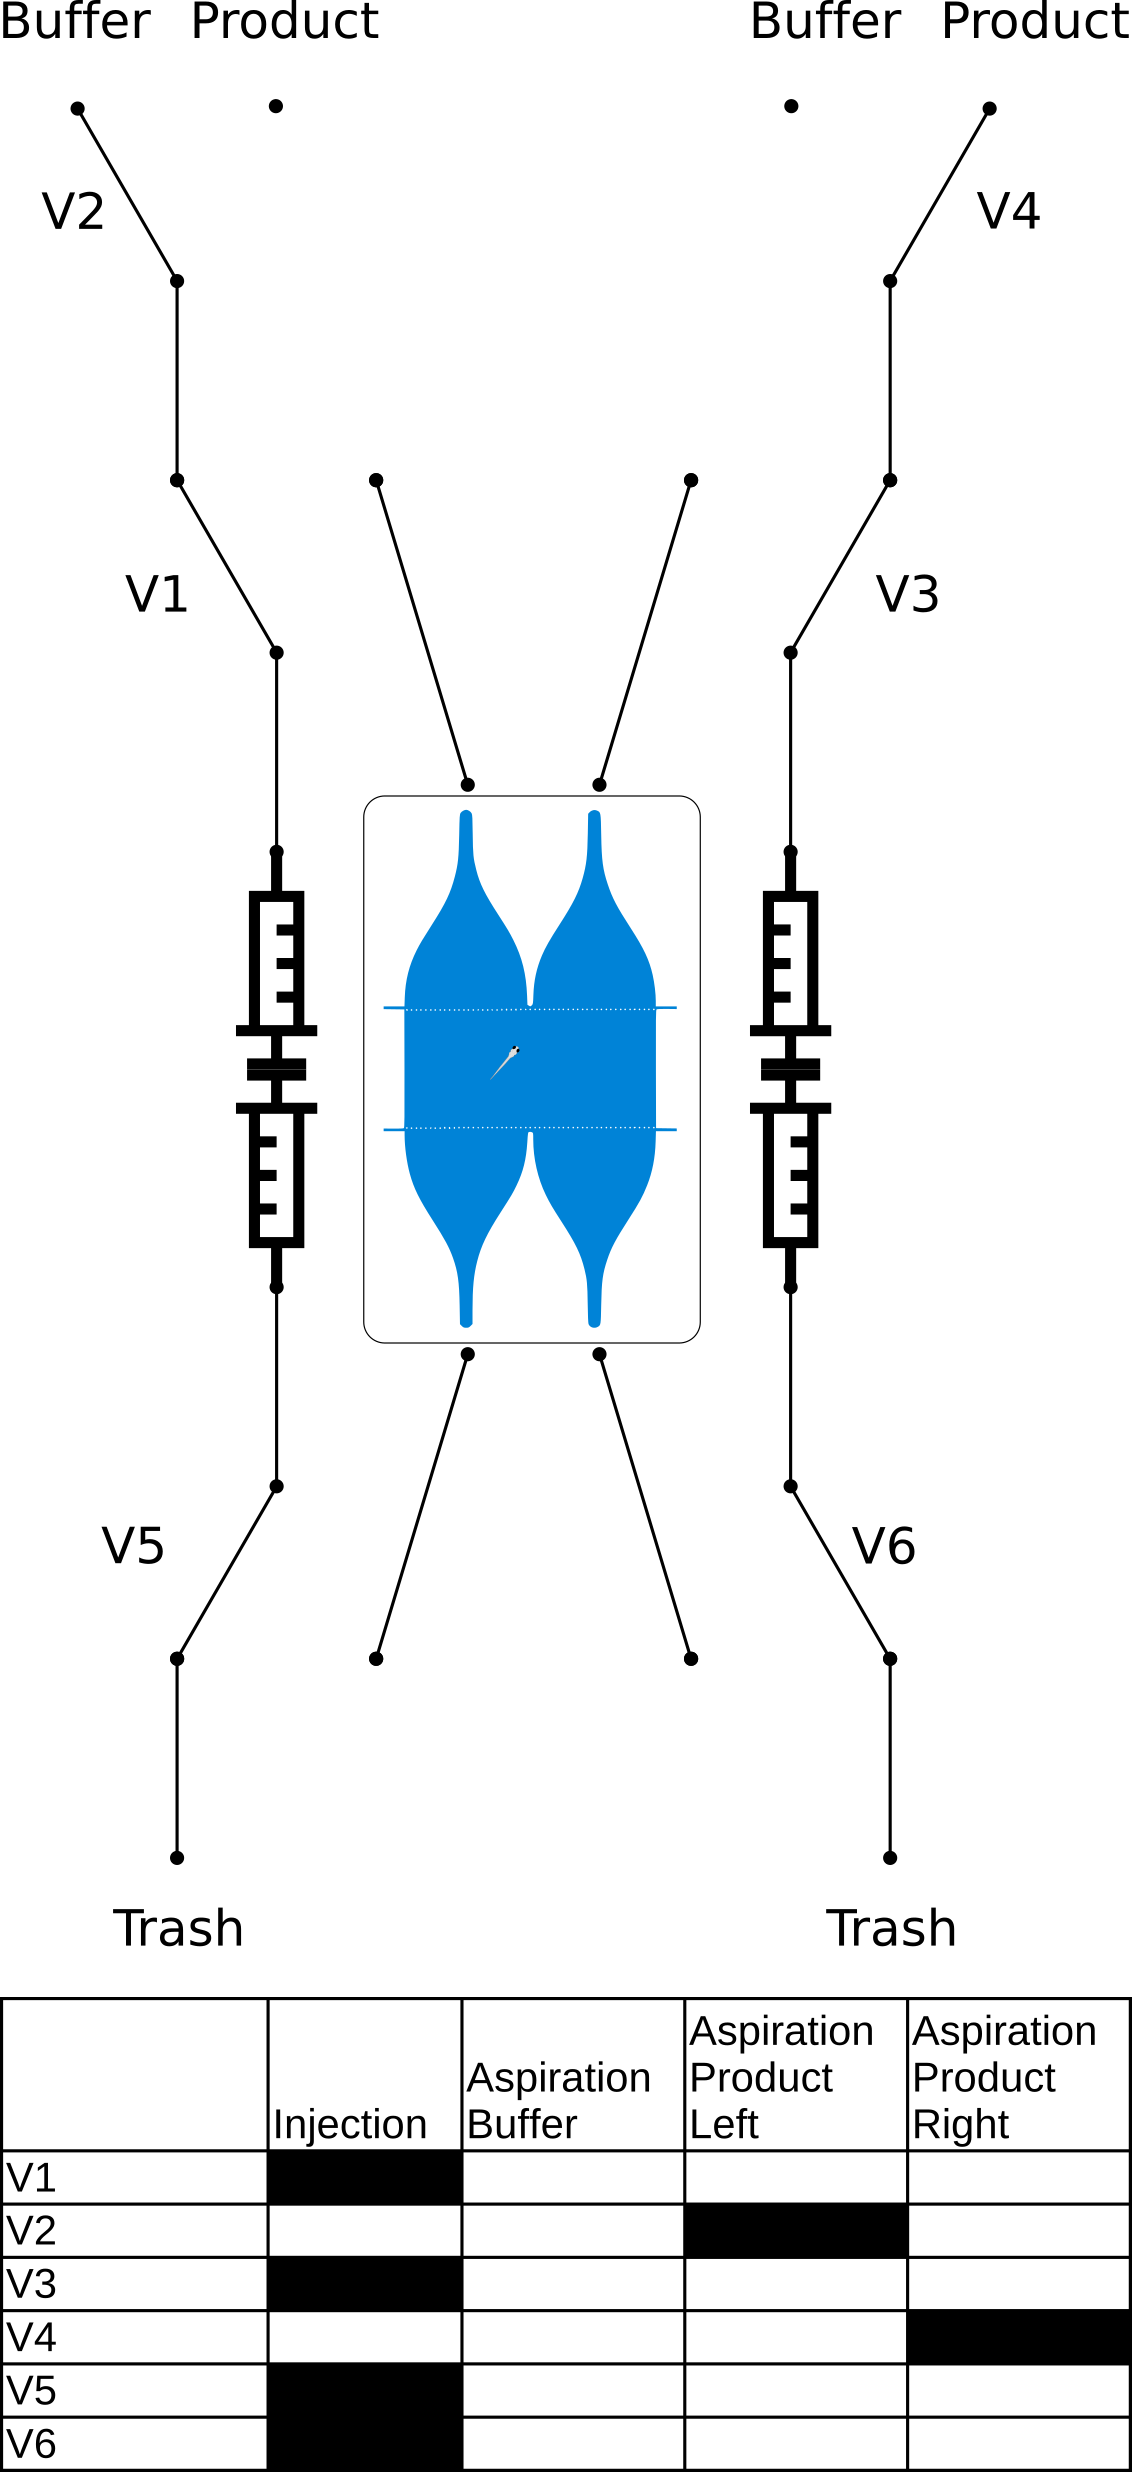
\includegraphics[width=0.50\textwidth]{part_2/assets/valve_schematic.png}
      \caption{\textbf{Valves manifold} \textbf{Top}: Valves system schematic. \textbf{Bottom}: Truth table of the system.}
      \label{valves_schematic}
    \end{figure}

  Sixty-milliliters syringes are fixed with 3D printed fixations on the actuator and connected with 2.2 mm diameters tubing to the microvalves circuit. Six three-ports microvalves are connected and form a circuit that allows performing cycles of filling and injection, see Figure~\ref{valves_schematic}.

    \begin{figure}[h]
      \centering
      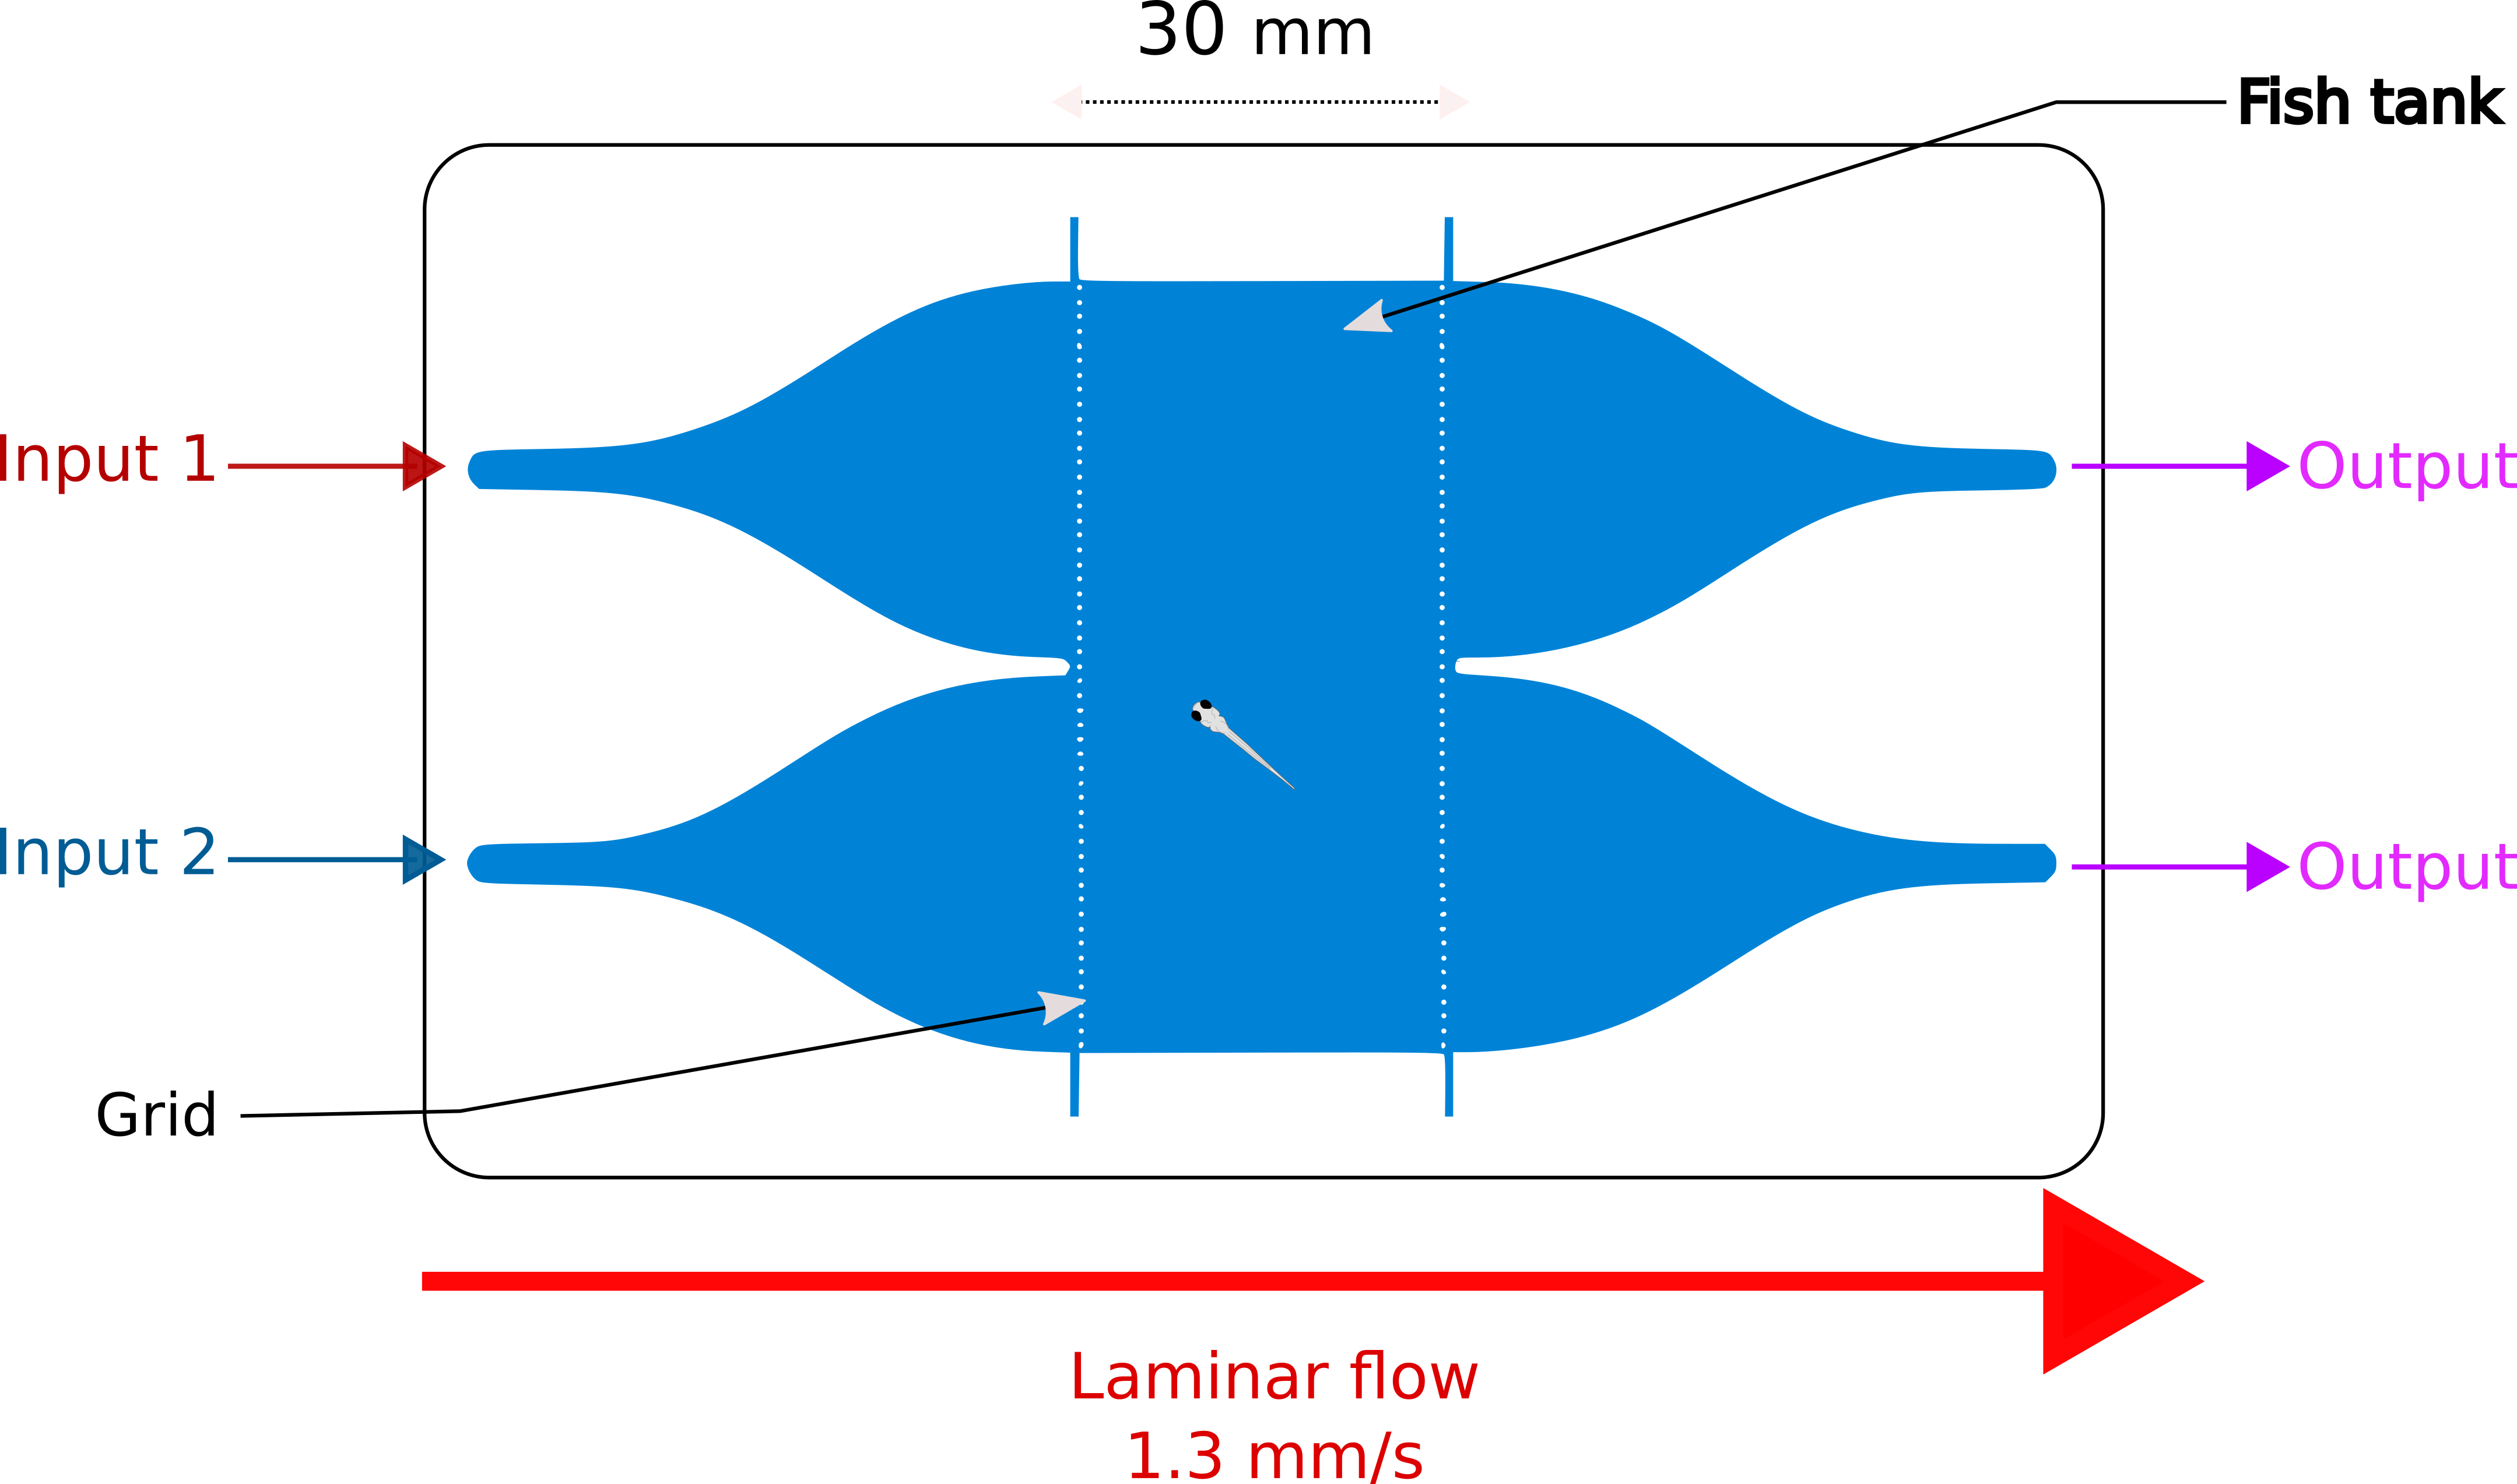
\includegraphics[width=0.75\textwidth]{part_2/assets/chip.png}
      \caption{\textbf{Millifluidic chip schematic.}}
      \label{dual_chip}
    \end{figure}

    \begin{figure}[h]
      \centering
      \includegraphics[width=0.75\textwidth]{part_2/assets/chipxcf.png}
      \caption{\textbf{Millifluidic chip exploded view.}}
      \label{dual_chip_visu}
    \end{figure}

  \subsubsection{Imaging}
  The setup is lightened by transmission using an infrared LED placed at the bottom of the box. Homogenous lighting is obtained by placing a diffusor (tracing papers or white plastic sheet) at the box's mid-height. Experiments are recorded with a Chameleon 3 camera mounted with a 23-25 mm EFL lens connected directly to the computer via USB3. A PMMA infrared transparent sheet is placed between the camera and the lens to block visible light and only retrieve Dual's infrared lightening.

  \subsubsection{Electronic}
  The electronic system links the analogic mechanical and millifluidic system to the software. A custom printed circuit board (PCB) has been designed for Dual. It contains an Arduino Nano microcontroller, six half H-bridges controlling the microvalves based on the logic signals of the Arduino; a Big EasyDriver stepper motor controller to control the motor speed from a logic output of the Arduino; a potentiometer to control the intensity of the LED lighting. All the electronics and the syringe pump motor are powered by a 550W ATX computer power supply connected to the PCB.

  \subsubsection{Software}
  A software has been specifically developed to control the setup. The graphical user interface is developed using Qt, and the camera is interfaced to the software using the FLIR Systems SDK provided with the camera. The electronic system is controlled through the Arduino Nano flashed with a custom sketch and communicating to the software via USB serial. The software allows manual control of each system element, such as the microvalves, the camera, and the motor. It is possible (and advisable) to create custom experimental protocols, a simple text file, containing the necessary instructions to automate the filling and aspiration cycles to build experiments.

  Two versions of the software are available, one running on a modern desktop computer that can drive four Dual, another running on a Raspberry Pi4 that drives only one Dual. The latest solution offers better scalability since each Dual is independent. A custom version of Ubuntu 20.04 is preinstalled with the camera's SDK and the software. It can be downloaded at \url{https://github.com/LJPZebra/dual_control/releases} and flashed on an SD card or USB device. It is designed to work with a 7-inch touchscreen display allowing a compact and easy-to-use control.

  \subsection{Construction and usage}
  For our needs, we have built four Duals that we ran in parallel, see Figure~\ref{dual_photo}. The construction requires a laser cutting machine, a 3D printer, and workshop tools. It took about two weeks to build the four devices. The construction does not require any specific knowledge, and access to a FabLab is sufficient to carry out this project and find the required tools and help in the event of difficulties.

  In practice, using Dual is effortless. Once the experiment template is created, the only manual task remaining is to place the fish in the millifluidic chip, close the device, and play the experiment template. It is also necessary to check that the suction containers neither run out of water or chemical. It is then possible to do experiments with minimal manual interventions.

  A recurring problem we have encountered is the fouling of the millifluidic system. The dye used to visualize the flow ends up clogging the valves and tubes and can stop the system in the middle of an experiment. This problem can be solved by taking preventive habits. After each day of experiments, the millifluidic system has to be flushed with water. It can be performed automatically using an experimental template designed to wash all the microvalves thoughtfully. Microvalves can regularly be passed in an ultrasonic bath to clean them. The tubes have to be changed when worn out, which can append after several weeks of intensive usage. Another encountered problem was the syringe plunger wear. After several months of usage, the plunger's latex cap loses water-tightness, and the plunger has to be replaced, which can be done very quickly in less than 2 minutes.

  In this project, we did not use all the Dual's potential. This setup can be adapted to other animals like adult Danionella a promising new model for neuroscience. It can assess other preferences, notably the preference to light (phototaxis) with the integrated visible LED.

  \section{The Tropical River}
  Studying chemical perception and chemically-driven navigation in a turbulent aquatic environment like the one fish encounters naturally requires an experimental device capable of creating controlled flows and chemical jets. We have created an experimental device capable of delivering a temperature-controlled laminar flow while recording the fish in both visible and infrared light. An injection nozzle is used to create turbulent or laminar jets within this laminar flow.

    \begin{figure}[h]
      \centering
      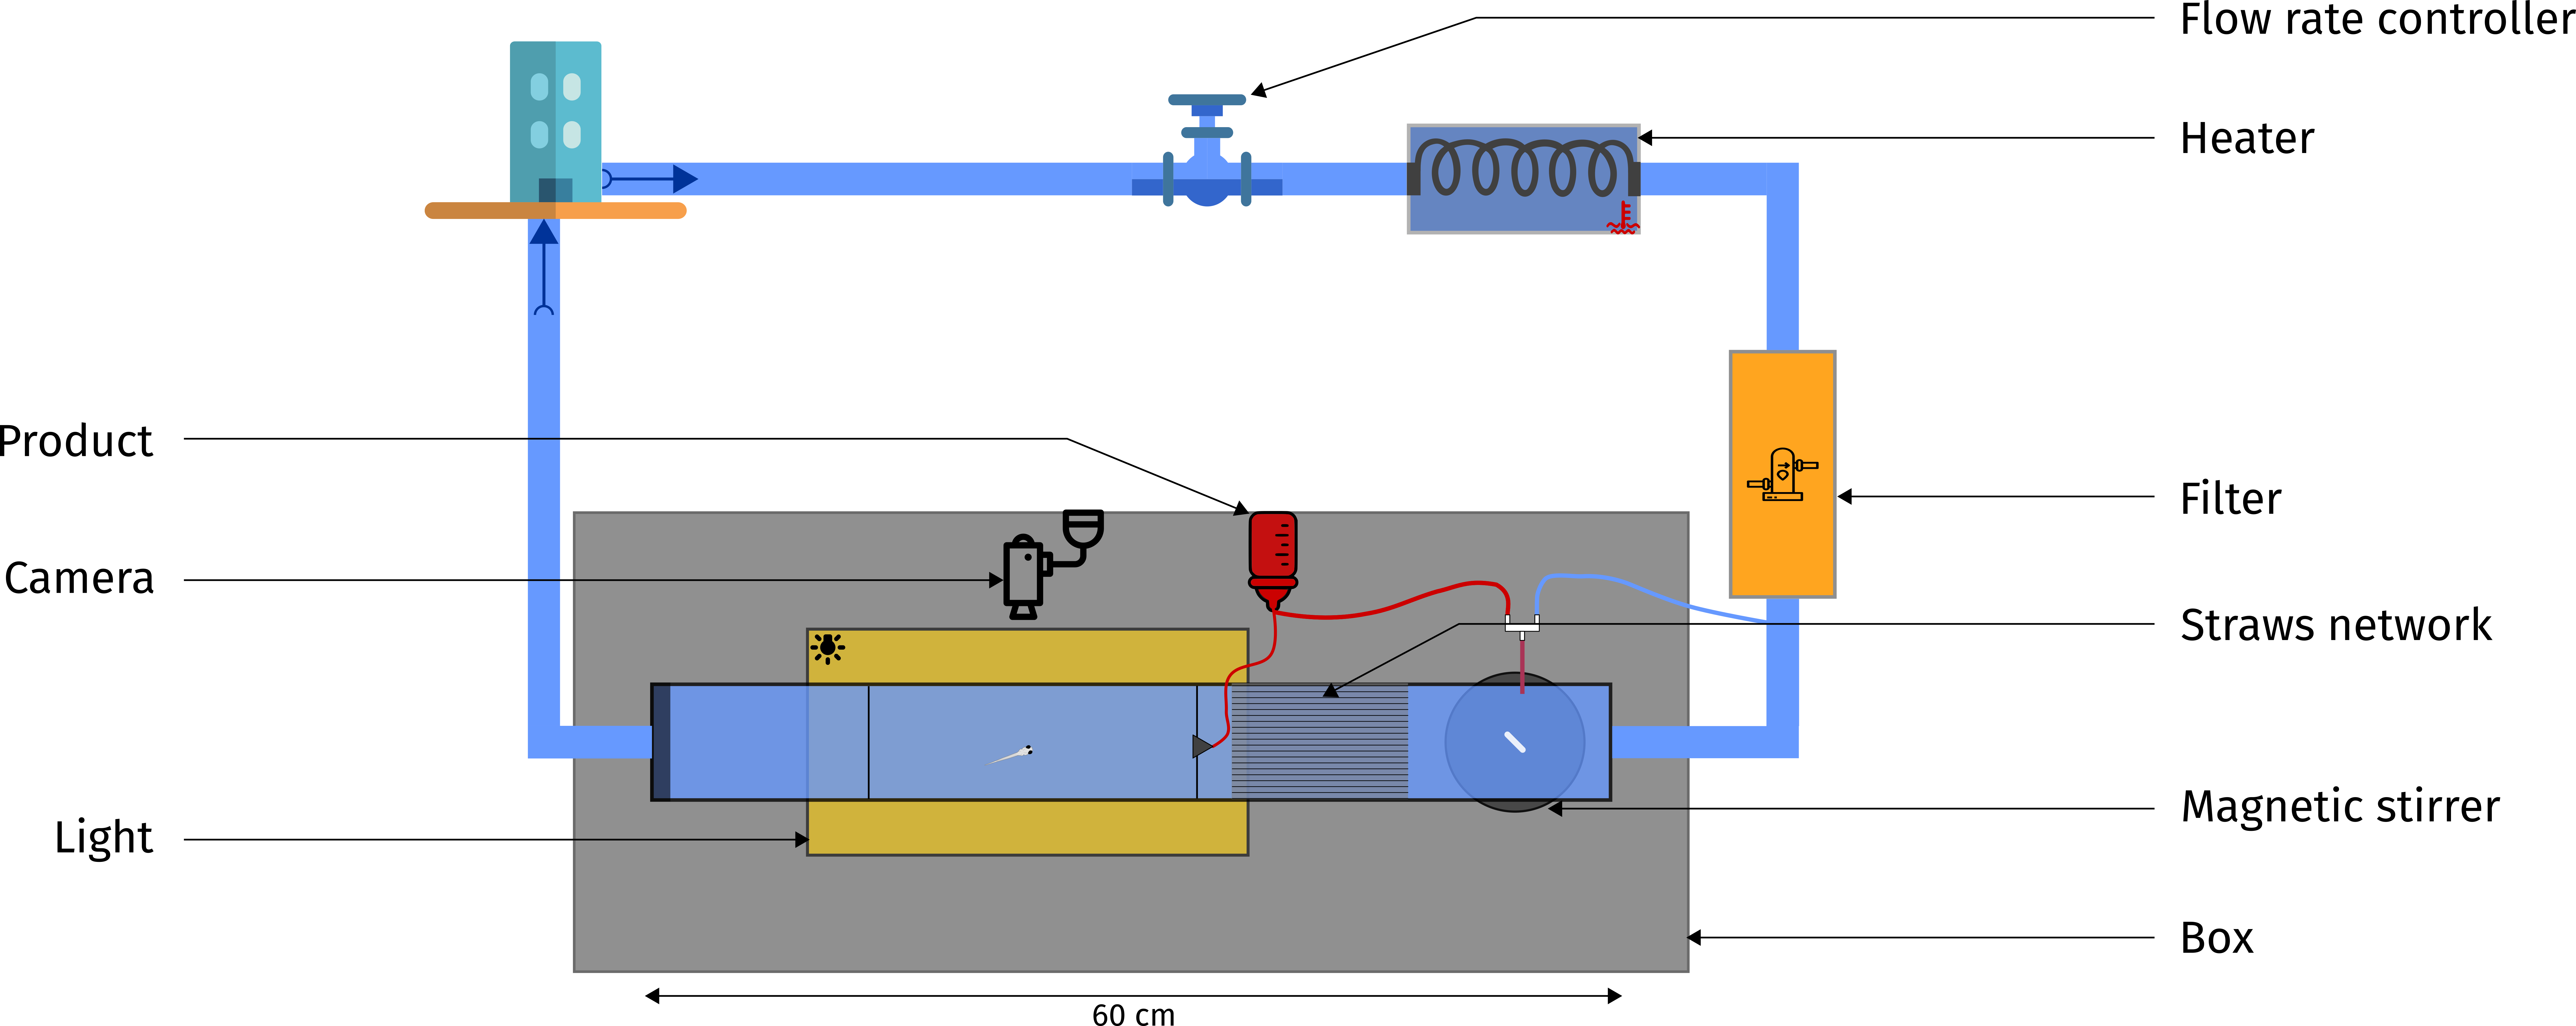
\includegraphics[width=1\textwidth]{part_2/assets/river.png}
      \caption{\textbf{The Tropical River} Schematic of the experimental setup.}
      \label{river}
    \end{figure}

\subsection{Description}
  \subsubsection{Structure}
  The device's structure consists of a channel assembled from transparent polycarbonate sheets machined precisely by the mechanical workshop and fixed with Norcan and Makerbeam rails to form a channel (60x10x10 cm), see Figure~\ref{river}. A LED panel is placed under the channel to illuminate the setup by transmission in visible light. The setup can be illuminated from above by a ring of infrared LEDs or by transmission by covering the LED panel with a PMMA infrared transparent sheet. A Chameleon 3 camera is placed above the channel to record the experiments and connected to the computer via USB3. A mirror is placed at 45 degrees of inclination from the horizontal on the channel's side to control the fish's vertical position. The whole channel is set inside a box constructed with Norcan rails and plywood sheets to isolate the fish from the surrounding environment.

  \subsubsection{Hydrodynamic}
  The canal is supplied at one end with water from the building's water system. Before entering the canal, tap water is filtered by an activated carbon filter and heated by a water bath. A network of straws is placed in the channel to obtain a laminar flow, and a solenoid valve can adjust the flow rate. The other end of the channel is left free. The outgoing water is redirected to the building's wastewater network because the products tested do not require any special treatment before being disposed of. The water height inside the channel can be controlled by modulating the dyke height placed at the end of the channel.

  It is possible to dilute a product inside the channel by using an injection nozzle located directly at the water supply outlet. A magnetic stirrer is placed inside the channel, before the straws network, to facilitate dilution. Another injection nozzle can be placed inside the channel, after the straws network, to create a turbulent or laminar jet. It is supplied by an external tank, and the flow rate can be adjusted by gravity and delivery automatically controlled by a valve system.

    \begin{figure}[h]
      \centering
      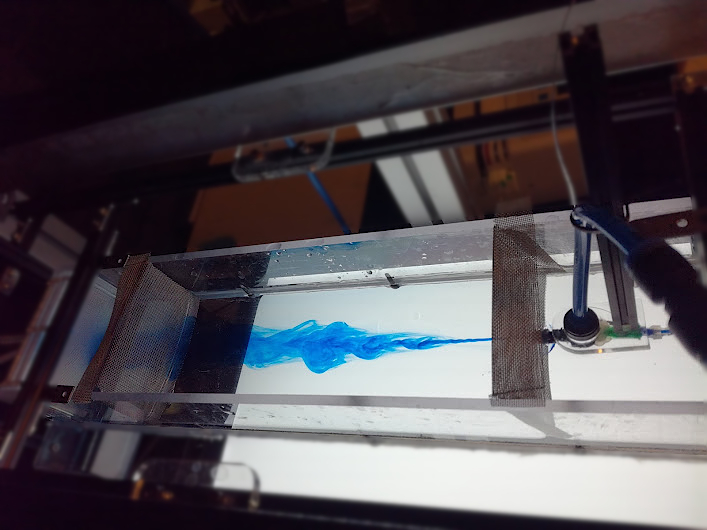
\includegraphics[width=0.80\textwidth]{part_2/assets/river_flow.jpg}
      \caption{\textbf{The Tropical River} Example of a turbulent jet visualized using blue visible colorant.}
    \end{figure}

  \subsubsection{Software}
  The control software allows to retrieve and control all the variables of the experiment. By default, it allows selecting the flow rate, temperature, injection valves, and camera settings. A vital function of the software is the ability to build experimental protocols. Easy to build, the protocol template is a simple text file specifying for a given device a variable's desired value at a given time point. Any Arduino sensor or control device that follows a convention detailed in \url{https://github.com/LJPZebra/the_tropical_river_control} can be called in these protocols without the need to modify the software.

  \subsubsection{Camera}
  The camera's options are directly accessible inside the software using the Spinnaker SDK. Metadata like temperature, relative times to the experiment, flow rate, or user-specified value can be saved inside the image.

  \subsubsection{Temperature}
  The temperature regulation is made using a coiled heat exchanger tube added to the water inlet and immersed into a Neslab RTE water bath capable of cooling and warming. A temperature sensor is placed inside the channel and sends the instantaneous temperature to the control software. The software can control the water bath via an RS232 serial connector selecting the temperature using a PID feedback system. Despite large variations of the building's water temperature, this system allows a precise and rapid temperature regulation.

  \subsection{Usage and limitation}
  This experimental device is, in practice, very versatile. The ability to control the velocity and the temperature of the laminar flow, as well as the injection of products in an automated and quantified manner while recording the fish, allows the study of a wide variety of behaviors like rheotaxy, chemotaxis, and thermotaxis. The height of water in the channel can be modulated, making it possible to use adult and larval fish in the same setup.

  The insertion of chemical in the flow does not allow us to reuse the water. This is why the water supply is done using the water network of the building. Although filtered, the water quality depends on the building's water quality, which is usually not a problem for juvenile and adult fish that are reared in filtered tap water from 2 weeks onwards. However, this can be more problematic for larvae, which are more fragile and require calibrated water. Although the experiment's duration is limited only by the computer's storage, small air bubbles appear in the channel after a few hours. This phenomenon is due to the dissolved gases present in the tap water and is detrimental to the fish. The activated carbon filter reduces this phenomenon, but it remains present and limits the maximum experimental time to a few hours.

\chapter{Results}
  \section{Methods}
  In the next sections, we will present the experimental protocol that we used and the analysis methods we developed to assess zebrafish chemical preference.

  \subsection{Experiment}
  \paragraph{Protocol} Fish chemical preference was assessed using Dual setup in a one-hour long experimental in a protocol detailed in Figure~\ref{exp_protocol}. This protocol is subdivided into four cycles of 15 minutes each:
\begin{itemize}
  \item B1: a cycle where buffer is injected on the two sides serving as a control.
  \item P1: a cycle where a product is injected on one side and buffer on the other.
  \item B2: same cycle as B1 in order to flush the system of any residual product.
  \item P2: same as P1 but with sides inverted.
\end{itemize}

    \begin{figure}[htb]
      \centering
      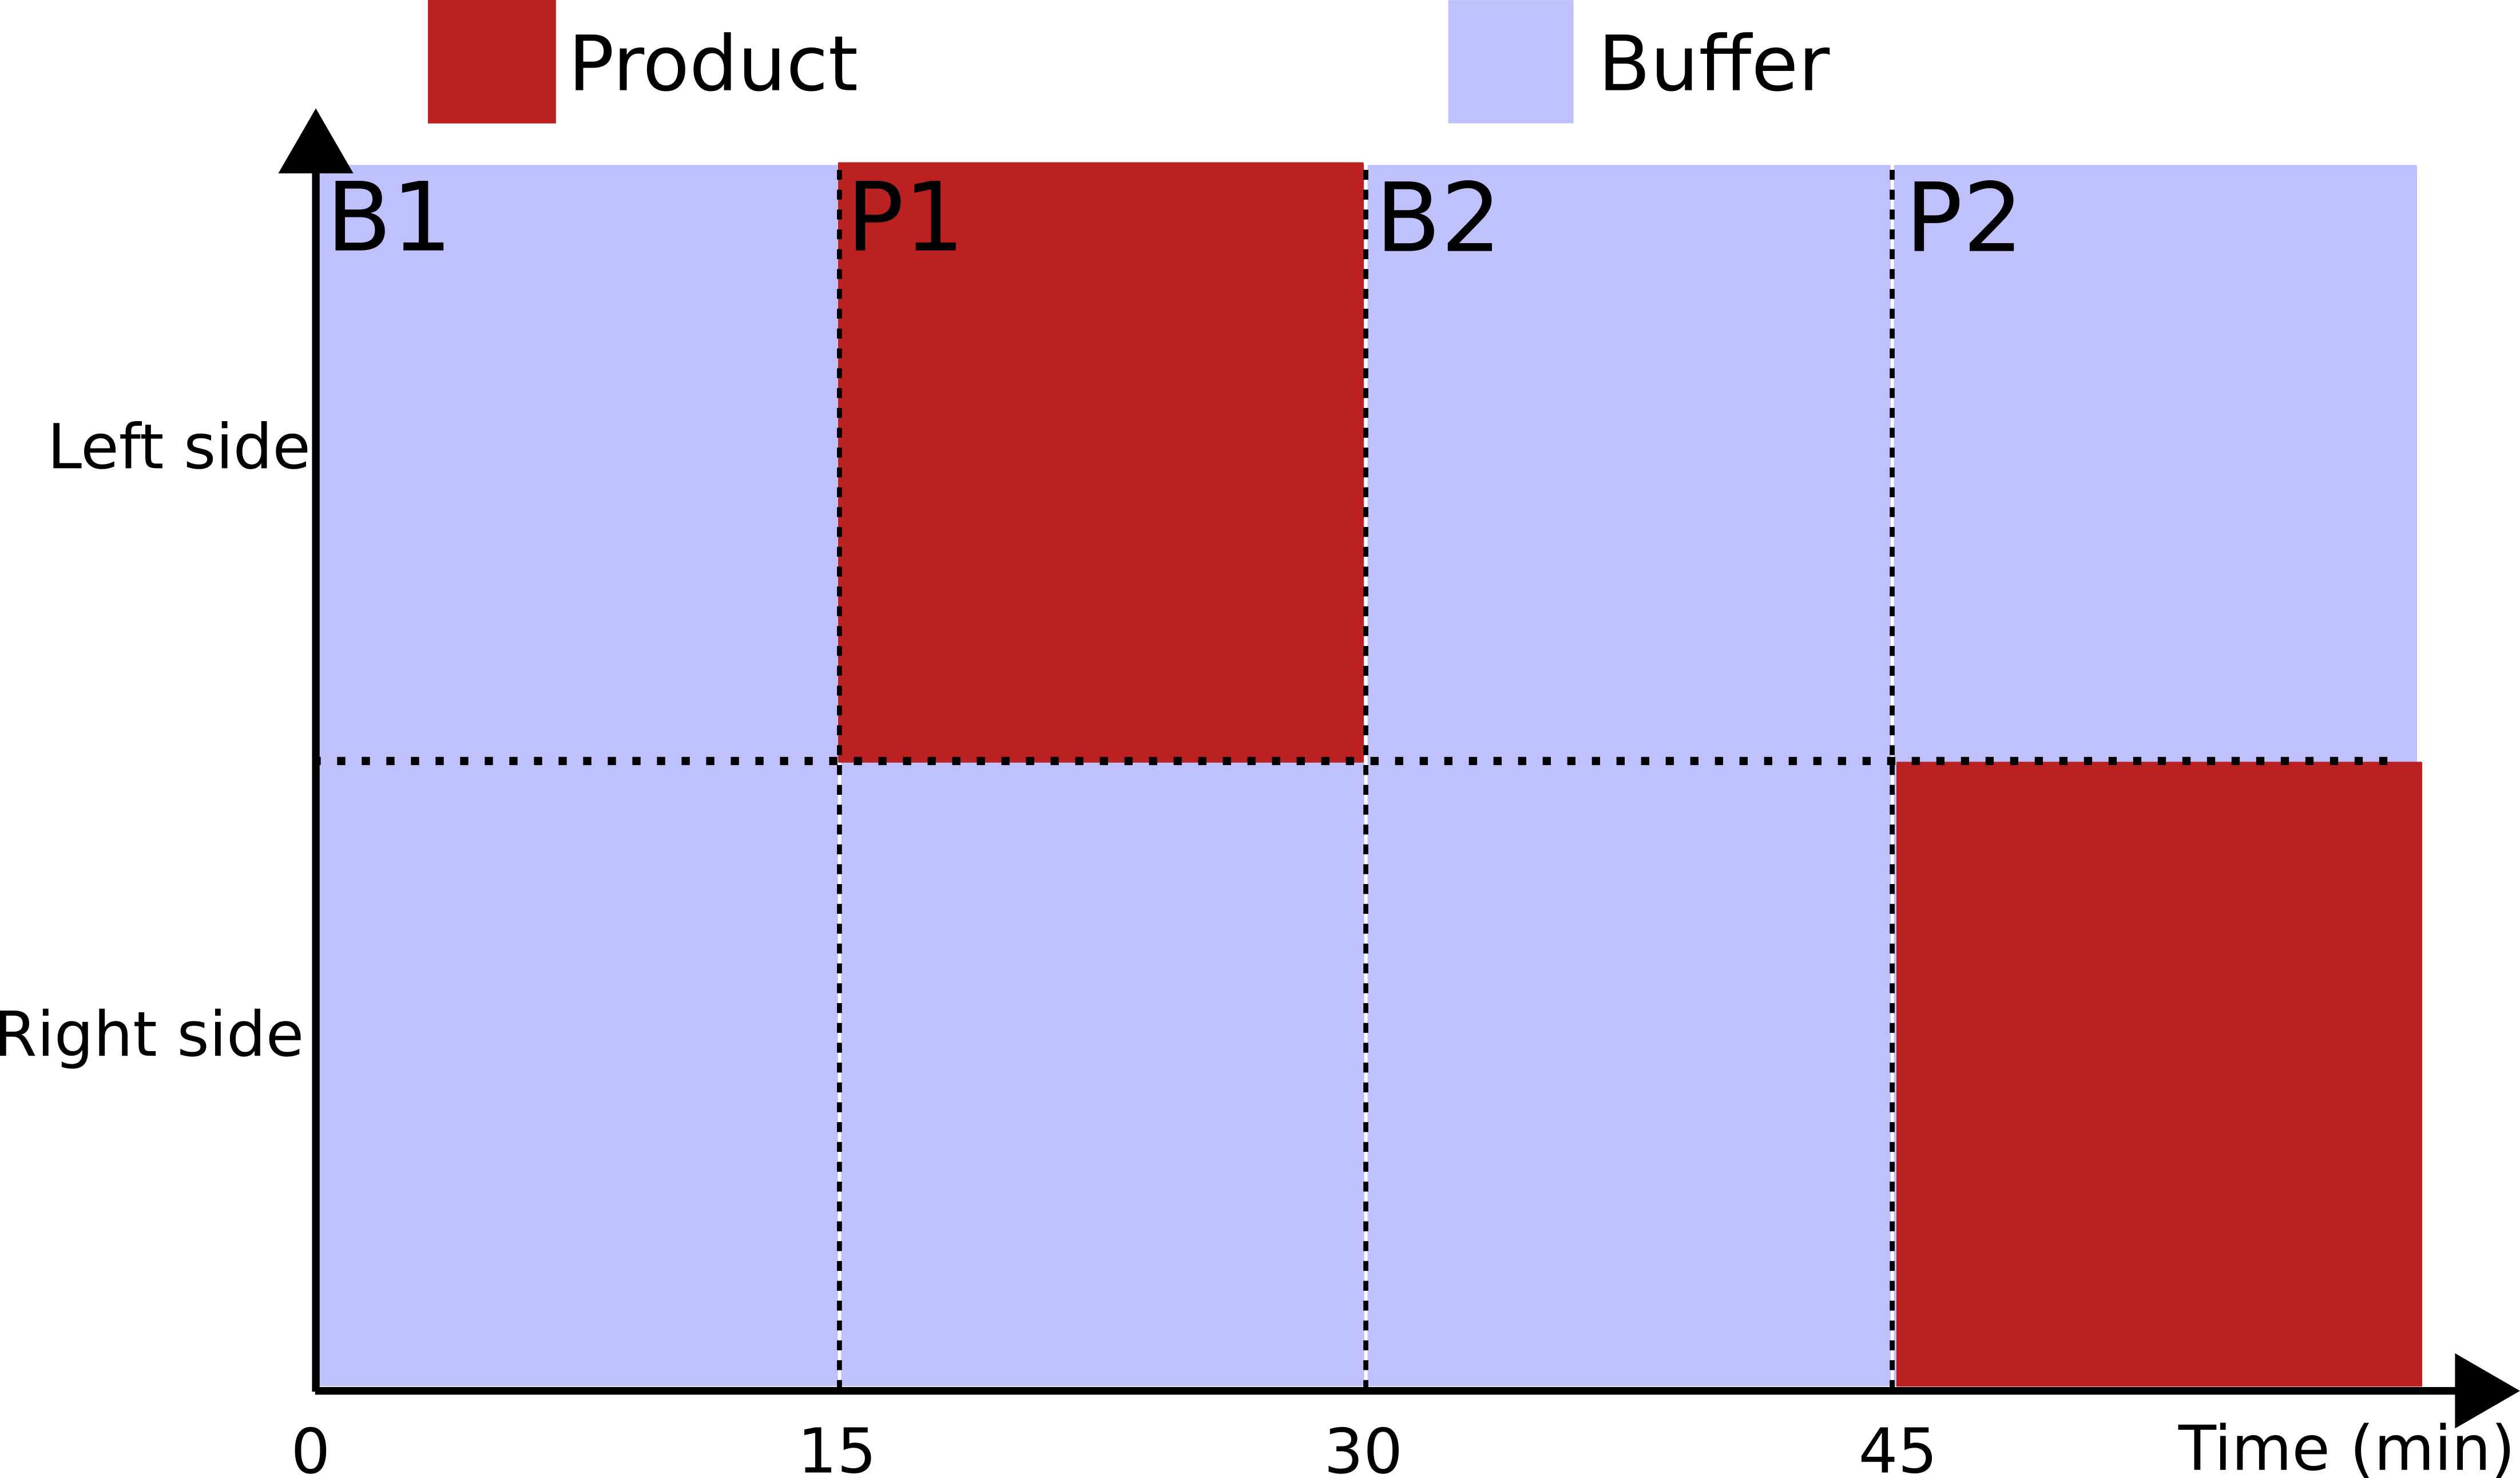
\includegraphics[width=0.75\textwidth]{part_2/assets/protocol.png}
      \caption{\textbf{Protocol} Experimental protocol used to assess zebrafish chemical preference. Product cycles P1 and P2 were regularly inverted to avoid any side bias.}
      \label{exp_protocol}
    \end{figure}

  \paragraph{Fish} In the following experiments, we use larval (6-8 days post-fertilization) and early juveniles (14 to 21 days post-fertilization) zebrafish. Preferences were assessed without changes in rearing condition before the experiment, except for ATP and adenosine, where fish were starved 24 hours before the experiment, a protocol inspired from \cite{wakisaka2017adenosine}. Chemicals were dissolved in a buffer the day of the experiment: E3 \footnote{\url{https://www.sc.niigata-u.ac.jp/biologyindex/natsuka/img/file26.pdf}} for larvae and degassed tap water for juveniles.

  \paragraph{Flow visualization} All experiments were performed in the dark to isolate the fish from non-chemical perceptions, especially visual perception. The flow was visualized using an infrared dye: an emulsion of silicone oil, sodium dodecyl sulfate, and alginate prepared by Lea-Laetitia Pontani. This emulsion contains droplets with a diameter of $5 \mu m$ with a polydispersity of $\approx 15 \%$ and is biocompatible \cite{ali2011large} at the concentration that we used ($\approx 500 \mu L/L$).

  \subsection{Analysis}
  The project's original idea was to use FastTrack (see Part~\ref{dual}) and an automatic custom-developed image analysis pipeline to monitor the fish preference using its position and recording the time spent in the product, see Appendix~\ref{auto_analysis}.

  \paragraph{Time-base preference index} The preference index is a measure of the attraction or repulsion of a product. It is defined from the times spent inside and outside the product as follows:
  \begin{equation}
    \Pi_{time}=\frac{t_{product}-t_{buffer}}{t_{product}+t_{buffer}}
  \end{equation}
  \noindent When $\Pi_{time} = 1$, the fish spend all its time on the product side; thus, the product is attractive. When $\Pi_{time} = -1$, it is the complete opposite, and the product is repulsive. $\Pi_{time} = 0$ means that the fish spent the same amount of time on each side; thus, the product is neutral.

  The critical point of this analysis method is to define when the fish is in the product. A coarse-grained analysis would be to assimilate the interface with its median position. Most of the time, it is accurate and robust to small inaccuracies. On the other hand, it will provide no insight at the crucial moment where the fish takes a decision, i.e., when the fish crosses the interface.

  To precisely understand the fish's behavior, we needed to record these decision events with low fault tolerance. Counting the contact events automatically between the interface and the fish proved to be very challenging due to the fish's complex behavior, see Figure~\ref{behavior_comp}, and the complexity of extracting the interface position based solely on the dye's contrast. A large amount of data and time constraints pushed us to develop a manual analysis method to count these events. The time spent manually counting these events was shorter than developing an automatic algorithm, then checking the result.

    \begin{figure}[htp]
      \centering
      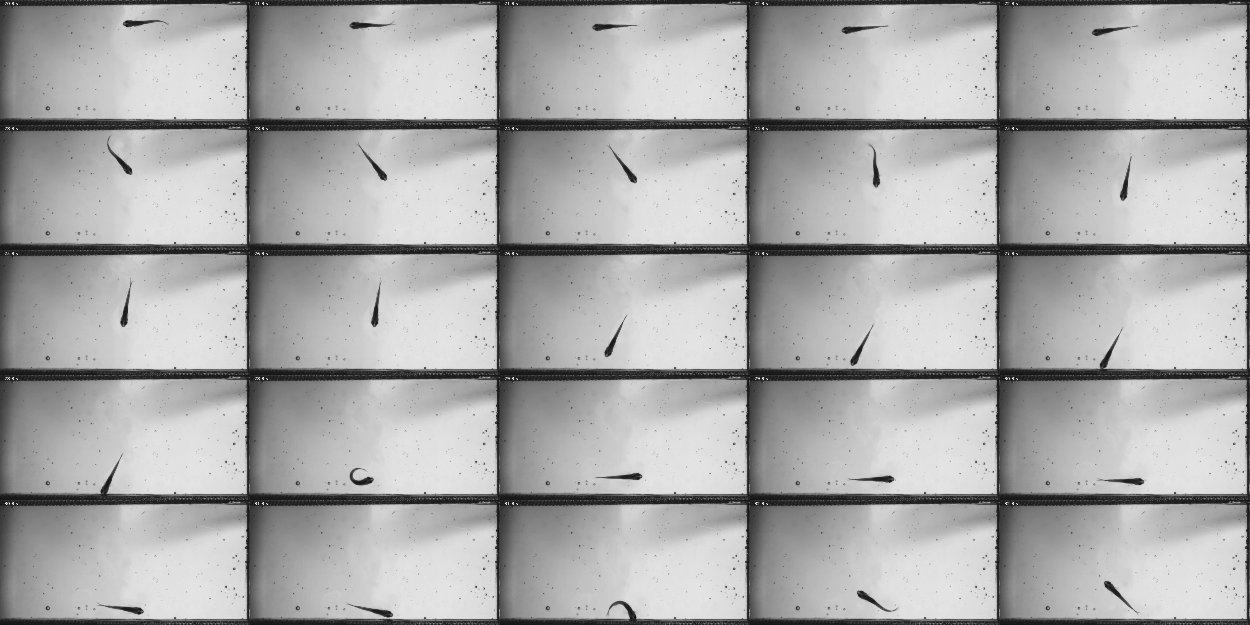
\includegraphics[width=1\textwidth]{part_2/assets/behavior.jpg}
      \caption{\textbf{Complexe behavior} Example of a complex behavior where the fish swim inside the interface. We see the product on the left side colored by the dye and the buffer on the right side. The fish is creating advection, and automatically extract the interface position is challenging. Pre-processed images where the background was substracted to enhance the contrast between the product and the buffer.}
      \label{behavior_comp}
    \end{figure}

  \paragraph{Event analysis} To develop the manual analysis method, we choose four characteristics and meaningful events to quantify the behavior, see Figure~\ref{events}. When the fish cross the interface to change side (PB: product to buffer and BP: buffer to product) and when the fish sense the interface and return to the side where it was (BB: buffer to buffer, PP: product to product). By recording these four events, we can quantify the moment where the fish make a decision, which was not possible with the time-based analysis.

    \begin{figure}[htb]
      \centering
      \includegraphics[width=0.75\textwidth]{part_2/assets/events.png}
      \caption{\textbf{Events} The event-based method of quantification distinguish 4 types of events that can occurs during P1 and P2 product cycles.}
      \label{events}
    \end{figure}

  To count these events, we performed a blind manual analysis where movies were anonymized and scrambled. The events counting was performed by two independents individuals and deanonymized then pooled together to get the average.

  We looked first at the correlation between the two independents analyses, see Figure~\ref{correlation_count}, to check for human bias. The correlation between each fish's events count was equal to $0.96$, indicating that there is no significant bias or disagreement between the analysis.

    \begin{figure}[htb]
      \centering
      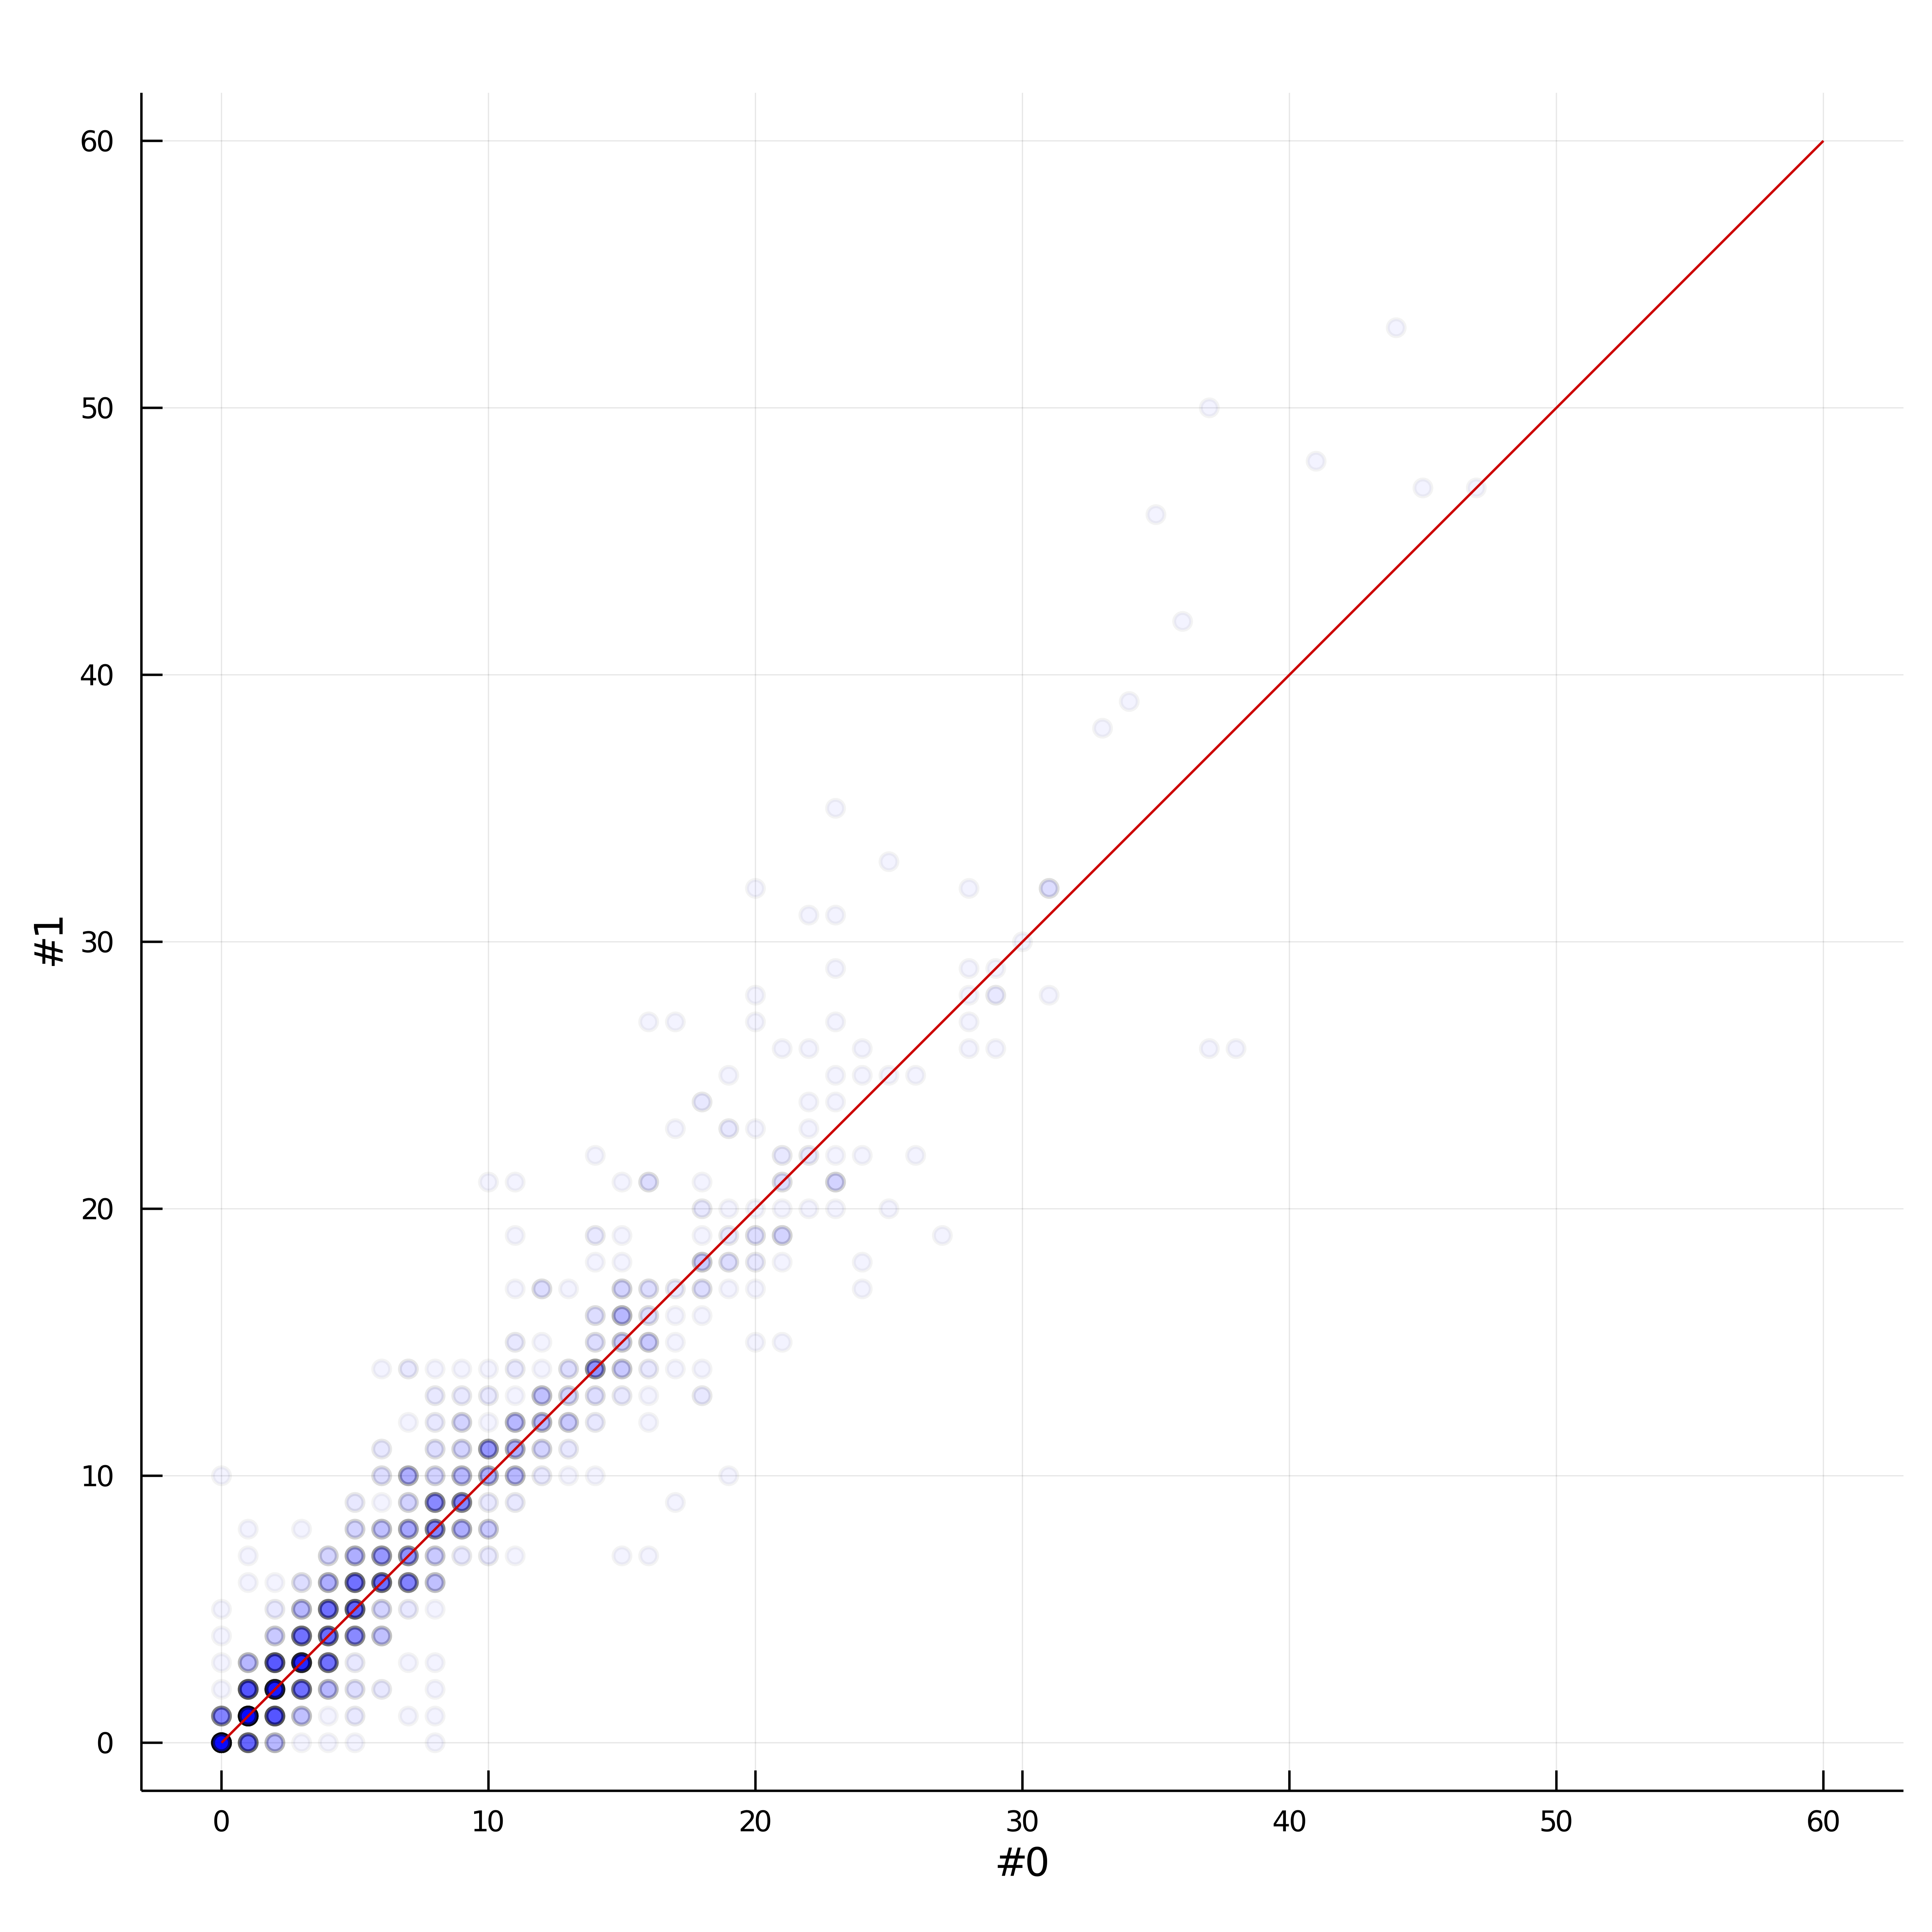
\includegraphics[width=0.65\textwidth]{part_2/assets/correlation.png}
      \caption{\textbf{Analysis correlation} Correlation between the two independent event-based analysis. One point is the count for one event type for one fish. Red line is the identity line. The point color intensity is encoding the number of points at the same coordinate.}
      \label{correlation_count}
    \end{figure}

  We can define an event-based preference index computed as the sum of the events finishing in the product minus the sum of events finishing in the buffer, divided by the total number of events:
  \begin{equation}
    \Pi_{event} = \frac{n_{BP} + n_{PP} - n_{BB} - n_{PB}}{n_{BP} + n_{PP} + n_{BB} + n_{PB}}
  \end{equation}
  \noindent This preference index is slightly different from the time-based one. It only reflects fish decisions and is not impacted by the fish inactivity and freezing.

  \paragraph{Ratio exploration-exploitation} Besides the preference of the fish, an interesting quantity that we can look at is the type of behavior. We can distinguish two modes of behavior: an exploration mode where the fish crosses the interface to explore the environment and an exploitation mode where the fish stays on the same side and make touch-and-turn at the interface (see Appendix~\ref{touch-and-turn} for more details). Note that this quantity is not by any means a preference indicator.

  The ratio exploration-exploitation can be computed based on the event recording as the number of events where the fish change side divided by the number of events where the fish stays on the same side:
  \begin{equation}
    \rho_{event} = \frac{n_{BP} + n_{PB}}{n_{BB} + n_{PP}}
  \end{equation}
\noindent When $\rho_{event} = 1$ there is as much exploration as exploitation, $\rho_{event} < 1$ there is more exploitation and $\rho_{event} > 1$ more exploration. In the case where $n_{BB} + n_{PP} = 0$ we take $\rho_{event} = 0$ (pure exploration),  and $n_{BP} + n_{PB} = 0$ we take $\rho_{event} = \infty$ (pure exploitation).

  \paragraph{Markov model} Based on the event recordings, we can build a two-state Markov chain model, see Figure~\ref{markov_model}. We can define the transfer probabilities as follows:
  \begin{equation}
    p = \frac{n_{BP}}{n_{BP} + n_{BB}} ;
    b = \frac{n_{PB}}{n_{PB} + n_{PP}}
  \end{equation}
  \noindent With $p$ the probability of going from the buffer to the product and $b$ the probability of going from the product to the buffer.

  \begin{figure}[h]
    \centering
    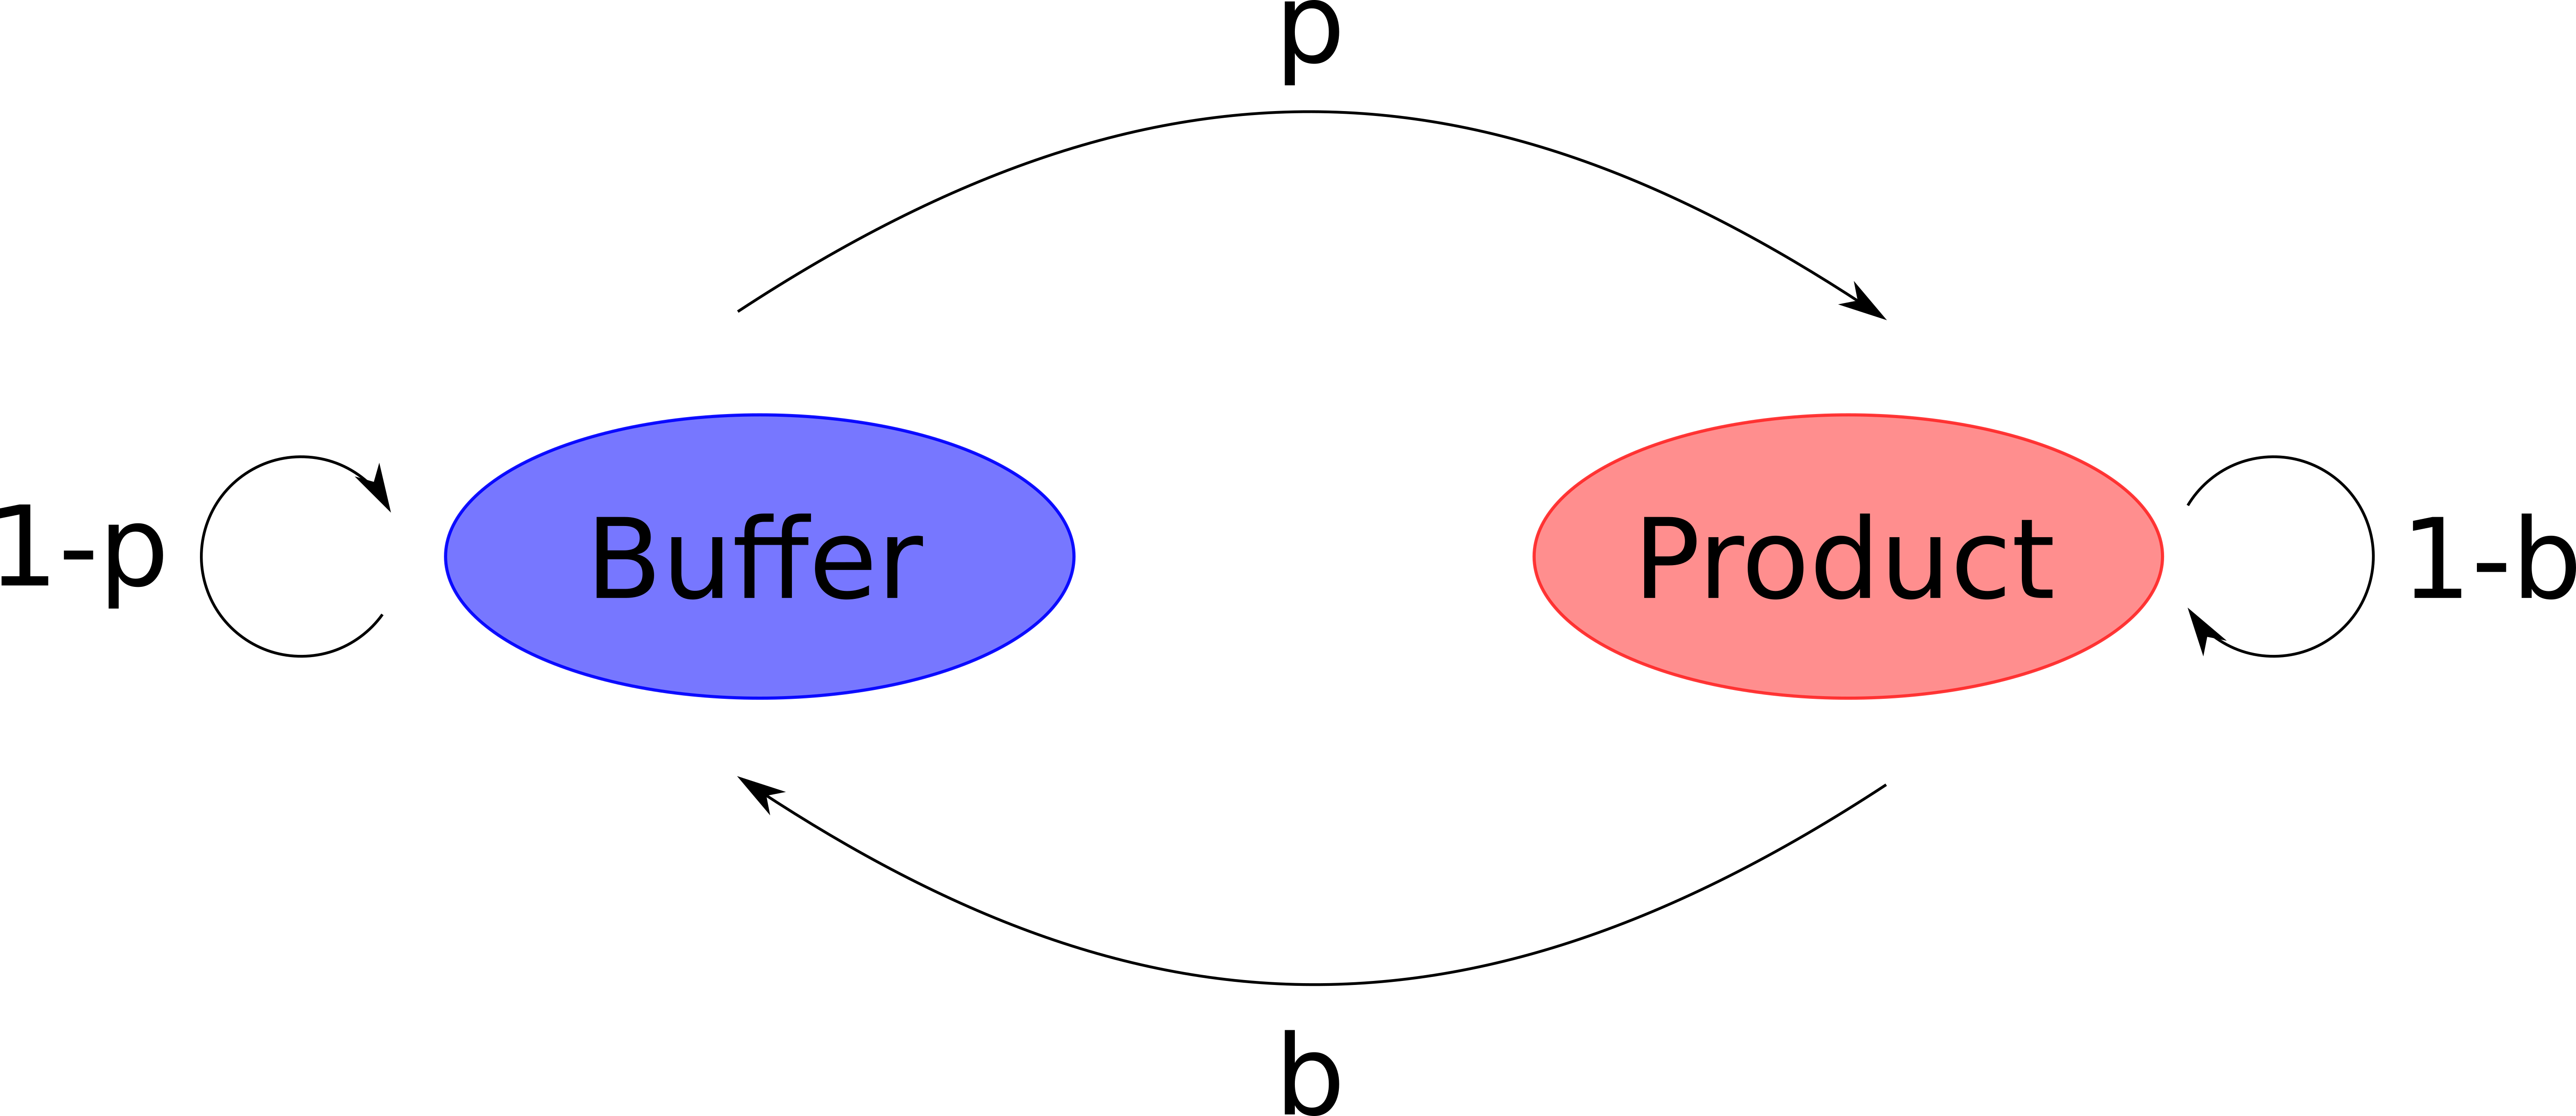
\includegraphics[width=0.85\textwidth]{part_2/assets/model.png}
    \caption{\textbf{Two states Markov chain model} P indicates the product state and B the buffer state.}
    \label{markov_model}
  \end{figure}

  This model offers yet another definition of the preference index defined directly by
  \begin{equation}
    \Pi_{Markov} = p - b
  \end{equation}
  \noindent the proportion of states product minus the proportion of states buffer. If $p$ (resp. $b$) cannot be defined, we take $\Pi_{Markov} = 1-2b$ (resp. $\Pi_{Markov} = -1+2p$).

 An indicator of the fish exploration-exploitation behavior can be derived as follows:
  \begin{equation}
    \rho_{Markov} = 2Min(p,b) - 1
  \end{equation}
   \noindent When $\rho_{Markov} = 1$,  the  behavior is purely exploratory, when $\rho_{Markov} = 0$ there is as many exploration than exploration and when $\rho_{Markov} = -1$ the behavior is dominated by exploitation.

  We can build a numerical simulation of a two states Markov chain to explore the relationship between $p$ and $b$ probabilities, $\Pi_{Markov}$, and $\rho_{Markov}$. The numerical simulation produces sequences generated from a Markov chain defined with probabilities $p$, and $b$. The length of the chain is drawn from the experimental chain length distribution that follows a discrete negative binomial distribution, see Figure~\ref{chain_fit}:
  \begin{equation}
    f(k) = \begin{pmatrix}
    k+n-1\\
    n-1
    \end{pmatrix}
    a^n(1-a)^k
  \end{equation}
  \noindent With $n=2.527$ et $a=0.084$.

  \begin{figure}[htb]
    \centering
    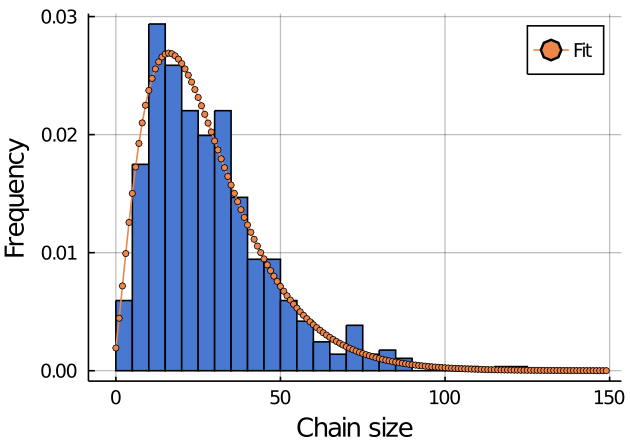
\includegraphics[width=0.75\textwidth]{part_2/assets/chain_fit.png}
    \caption{\textbf{Chain length} Experimental chain length distribution.}
    \label{chain_fit}
  \end{figure}

  We see in Figure~\ref{markov_simu} that there are forbidden couples of $(p,b)$ due to the definition of the probabilities $p$ and $b$ as rational numbers and the limited chain lengths. The preference indexes are distributed on either side of the identity line $p=b$ where $\Pi_{Markov} = 0$ with an upper triangle repulsive and a lower triangle attractive. Looking at the map of $\rho_{Markov}$, we see a right upper corner at high $p$ and $b$ dominated by exploration, and a bottom left corner by exploitation. As expected, the fish can have a neutral preference with either exploration or exploitation, but a strong preference can only happen in a regime dominated by exploitation.

  \begin{figure}[htb]
    \centering
    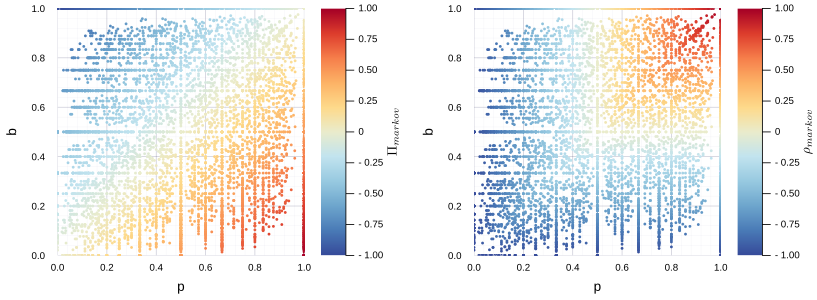
\includegraphics[width=1\textwidth]{part_2/assets/pi_pb.png}
    \caption{\textbf{Numerical simulation} Preference index $\Pi_{Markov}$ (left) and $\rho_{Markov}$ (right) for 10 000 realisations with a chain size following the experimental distribution.}
    \label{markov_simu}
  \end{figure}

  \section{Results}
  \subsection{Setup caracterisation}
  \paragraph{Left-right bias} We started by checking the preference index $\Pi_{time}$ in the B1 buffer cycle to capture an eventual left-right bias of setup. There is buffer on the two sides in this control cycle, and fish were never exposed to any product. We computed the time-based preference index choosing the middle of the tank as left-right separation (in B1, there is no dye, thus no other means to define separation). Figure~\ref{ld_bias} presents the distribution of time-based preference index for B1 cycles for larvae and juveniles. The first thing we can notice is the significant variability among fish. The median value ($\Pi_{time} = 0.08$ for $N=125$ for larvae and $\Pi_{time} = 0.05$ for $N = 178$ juveniles) is close to zero which allows us to exclude any systematic left-right bias of the setup.

    \begin{figure}[htb]
      \centering
      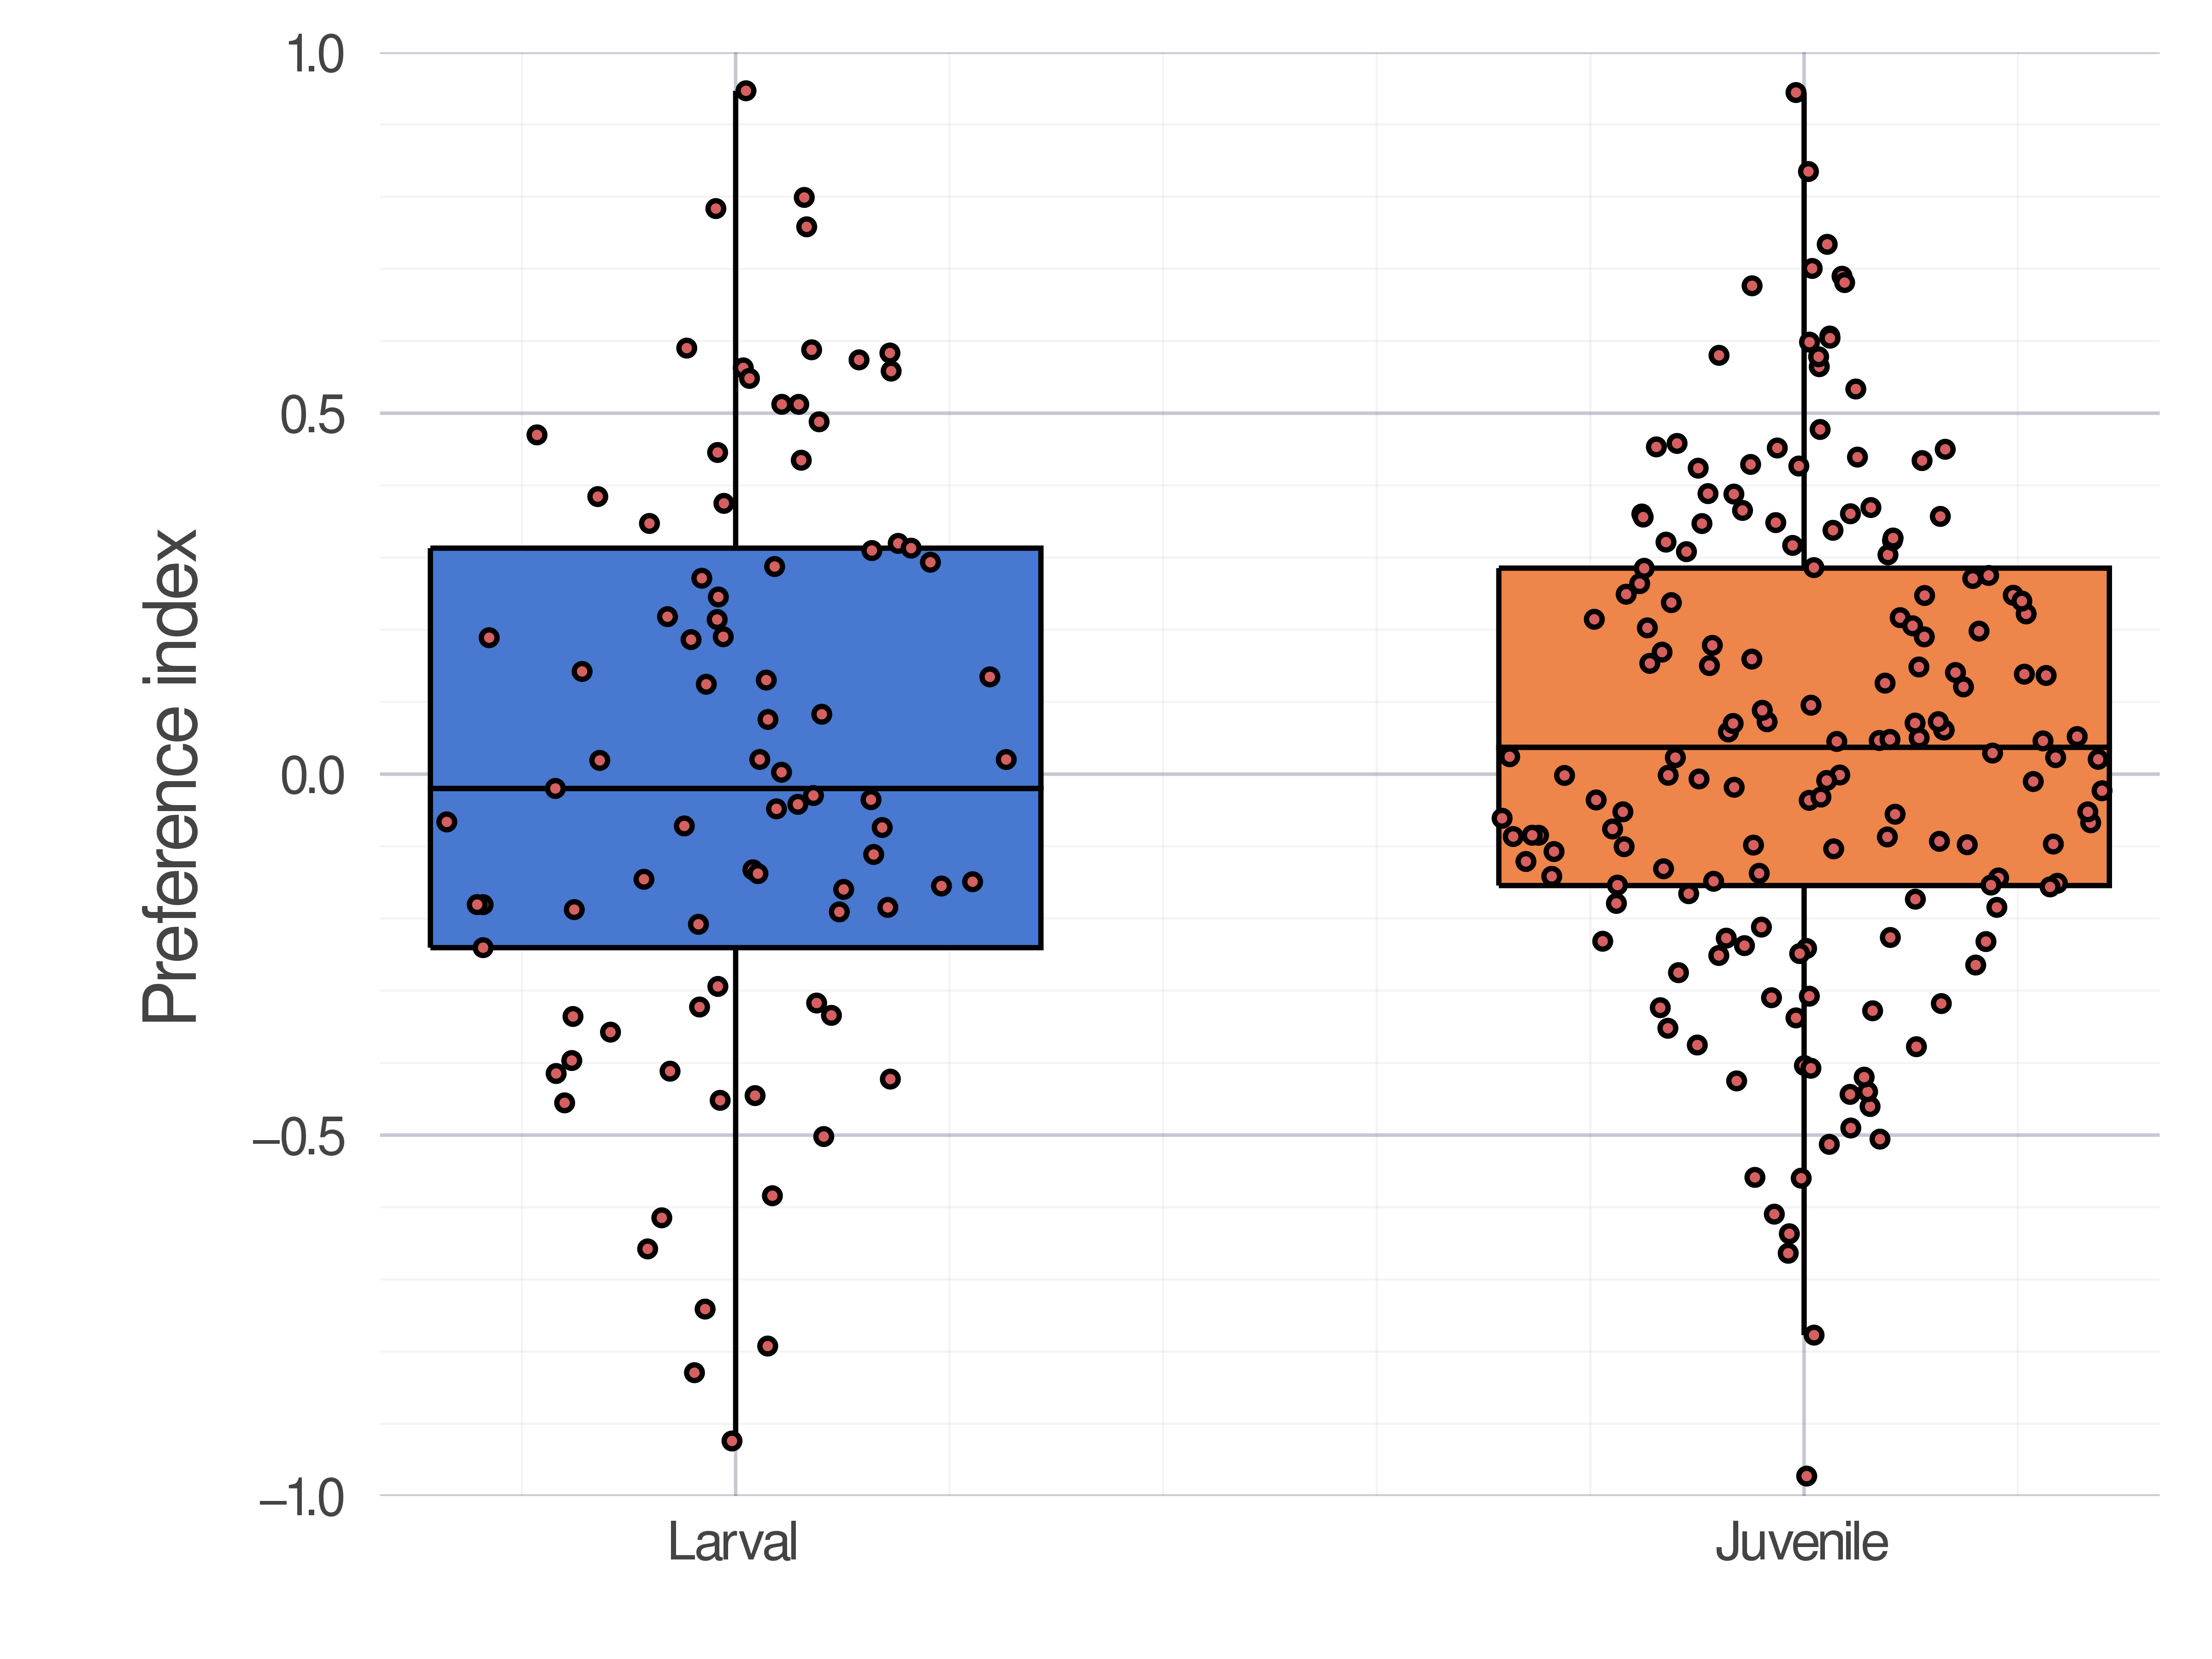
\includegraphics[width=0.75\textwidth]{part_2/assets/ld_bias.png}
      \caption{\textbf{Left-right bias} Distribution of the time-based preference index $\Pi_{time}$ computed for the first buffer cycle (B1) with buffer on the two sides. Each point is a value of preference index for one fish. Black line is the distribution median.}
      \label{ld_bias}
    \end{figure}

  \paragraph{Dye neutrality} In the product cycles P1 and P2, the dye is diluted with the product to visualize the flow. To study the dye's impact on the fish, we performed control experiments with juvenile fish assessing only the dye with the protocol presented above.

  Figure~\ref{dye_bias}A presents the event-based preference index $\Pi_{event}$ for the dye only. Each point is a fish analyzed by one person, and the point's size encodes the number of events during the cycle. We see that the dye seems neutral to the fish with no clear attraction or repulsion. As expected, there is large inter-fish variability. The preference index distributions for P1 and P2 are not statistically significant, but cycle P2 includes more outliers fish with strong preferences.

  Figure~\ref{dye_bias}B presents the time-based preference index $\Pi_{time}$, each point is representing one fish. We see a slight repulsion in the P1 cycle and a slight attraction in the P2 cycle towards the dye, but there is no clear, robust preference. These slight preferences are not visible with the event-based analysis. They are probably due to the time-based analysis's low precision with low statistics ($N=13$) because it is more sensible to periods where the fish do not make any decision.

  Figure~\ref{dye_bias}C presents the $p$ and $b$ probabilities from the Markov chain model by fish. In each cycle, we see that $p \approx b \approx 0.65$ differs from $1$, meaning that the fish can presumably perceive the dye or at least the side change by another unknown mean like a variation in flow velocity at the interface. This effect is also visible on the ratio exploration-exploitation $\rho_{event}$, see Figure~\ref{dye_bias}D that is close to $1$.

  Altogether, these results indicate that the fish can sense the dye but without manifesting any preference. With enough statistics to mitigate the fish inter-variability, we will be able to assess the fish preference while visualizing precisely the flow.

    \begin{figure}[H]
      \centering
      \includegraphics[width=1\textwidth]{part_2/assets/dye_pi.png}
      \caption{\textbf{Dye bias} \textbf{A.} Event-based preference index $\Pi_{event}$, one point is one fish analysed by one person ($2N$ fish). \textbf{B.} Time-based preference index $\Pi_{time}$, one point is one fish. \textbf{C.} $p$ and $b$ probabilities from the Markov chain model, one point is one fish analysed by one person ($2N$ fish). \textbf{D.} Ratio exploration-exploitation $\rho_{event}$, one point is one fish analysed by one person ($2N$ fish).}
      \label{dye_bias}
    \end{figure}

  \subsection{Products screening}
  We have screened several products reputed to elicit an aversion or attraction with zebrafish. Our study focuses mainly on early juvenile (14 days) zebrafish with preliminary results for larvae (7 days).

  \paragraph{Juvenile zebrafish in citric acid}
  Citric acid is known to be repulsive in many fish species. It was shown that adult zebrafish could sense their environment pH \cite{abreu2016acute,abreu2016behavioral} and display a strong aversion for acidic pH ($pH \approx 3$). As a positive control, early juveniles and larval zebrafish preference were assessed using citric acid solutions ranging from $5 \times 10^{-3} M$ to $1 \times 10^{-6} M$, ie pH from $2.8$ to $4.2$ (Figure~\ref{citric_acid}).

    \begin{figure}[h!]
      \centering
      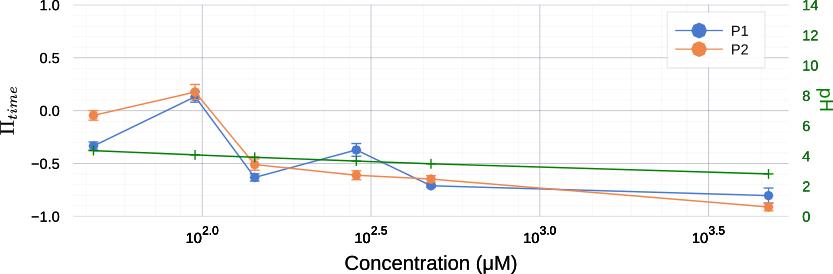
\includegraphics[width=1\textwidth]{part_2/assets/citricacid.png}
      \caption{\textbf{Citric acid: time-based preference index for juveniles} Time-based preference index (mean $\pm$ SEM, equation~\ref{mean_pi_time}), calculated pH in green.}
      \label{citric_acid}
    \end{figure}
    \begin{figure}[h!]
      \centering
      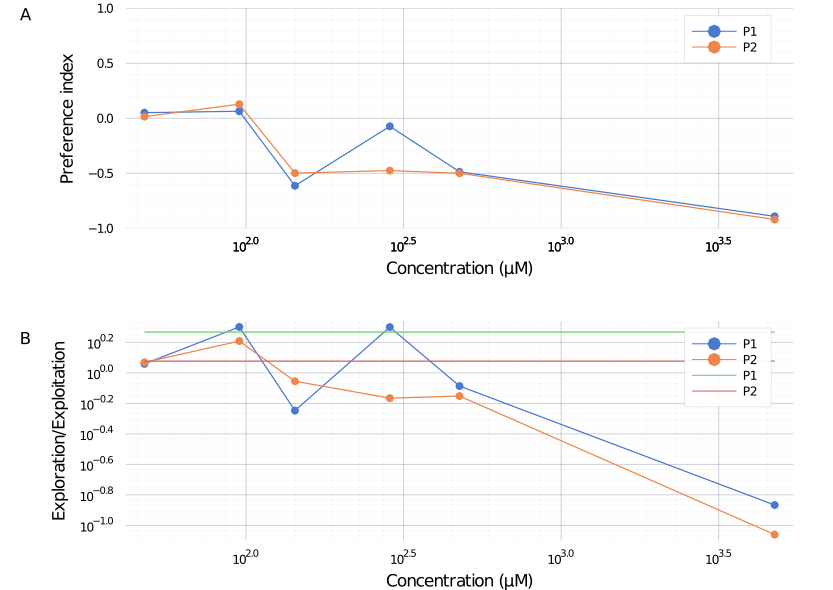
\includegraphics[width=1\textwidth]{part_2/assets/citricacid_event.png}
      \caption{\textbf{Citric acid: event-based analysis for juveniles} \textbf{Top}: Mean event-based preference index (equation~\ref{mean_pi_event}). \textbf{Bottom}: Mean ratio exploration-exploitation (equation~\ref{mean_r_event}).}
      \label{citric_acid_event}
    \end{figure}

  The mean ratios exploration-exploitation presented in Figures~\ref{citric_acid_event}~bottom and Figure~\ref{citric_acid_markov}~bottom, showed an apparent decrease when the citric acid concentration increase. Fish can sense citric acid and reduce their exploration to the benefit of a stereotyped exploitation behavior where they often go to the interface and return in the buffer.

  The time-based $\Pi_{time}$ (Figure~\ref{citric_acid}~top), event-based $\Pi_{event}$ (Figure~\ref{citric_acid_event}~top), and Markov-based $\Pi_{Markov}$ (Figure~\ref{citric_acid_markov}~top) mean preference indexes decrease in a concentration-dependent manner. The distributions of preference indexes by fish (Figure~\ref{dist_citric_acid}) show a decrease in variability as the concentration increase and no significant difference between P1 and P2 cycles, which tends to suggest that fish adopt the same characteristic behavior with less variability as a preference emerged.

  We tried to see if the bulk-behavior (i.e., modulation of the kinematic parameters inside the product) was able to explain the time-based preference index. We extract the parts of trajectory inside the product and the buffer during the P1 and P2 cycle and inside buffer in the B1 cycle as a control. Larvae and juveniles swim in units called bouts separated by rest periods called interbouts. We discretized the trajectory by swim-bouts and extracted three kinematic parameters: the time $\delta t$, the distance $\delta r$, and the angle $\delta \theta$, between the onset of successive bouts.

  It was shown by \cite{benichou2005averaged} that the mean escape time of a domain with a mix of reflective and absorbing walls by a random walker moving with constant velocity and changing directions at random times writes :
  \begin{equation}
    \label{eq_t}
    \left< t \right> = \alpha \frac{V}{vS}
  \end{equation}
  \noindent with $V$ the volume and $S$ the surface of the domain, $\alpha$ a numerical coefficient, and $v$ the velocity of the random walker.

  In our case, Dual can be seen as a domain of characteristic size $a$ with reflective walls (Dual edge) and an absorbing wall (the interface between product and buffer), see Figure~\ref{random_dual}~left. The fish trajectory can be seen as a random walk with a reorientation at each swim-bout. We see on Figure~\ref{random_dual}~right that $\delta t$ and $\delta r$ are uncorrelated and that there is a timescale $\tau$ and a lengthscale $\lambda$ such as:
  \begin{equation}
    \label{eq_vel}
    \left< v \right> = \frac{\lambda}{\tau}
  \end{equation}
  \noindent and with Equation~\ref{eq_t},~\ref{eq_vel} and $\frac{V}{S}=a$ in Dual we have:
  \begin{equation}
    \label{eq_tmean}
    \left< t \right> \approx \alpha \frac{a \tau}{\lambda}
  \end{equation}.

      \begin{figure}[h!]
        \centering
        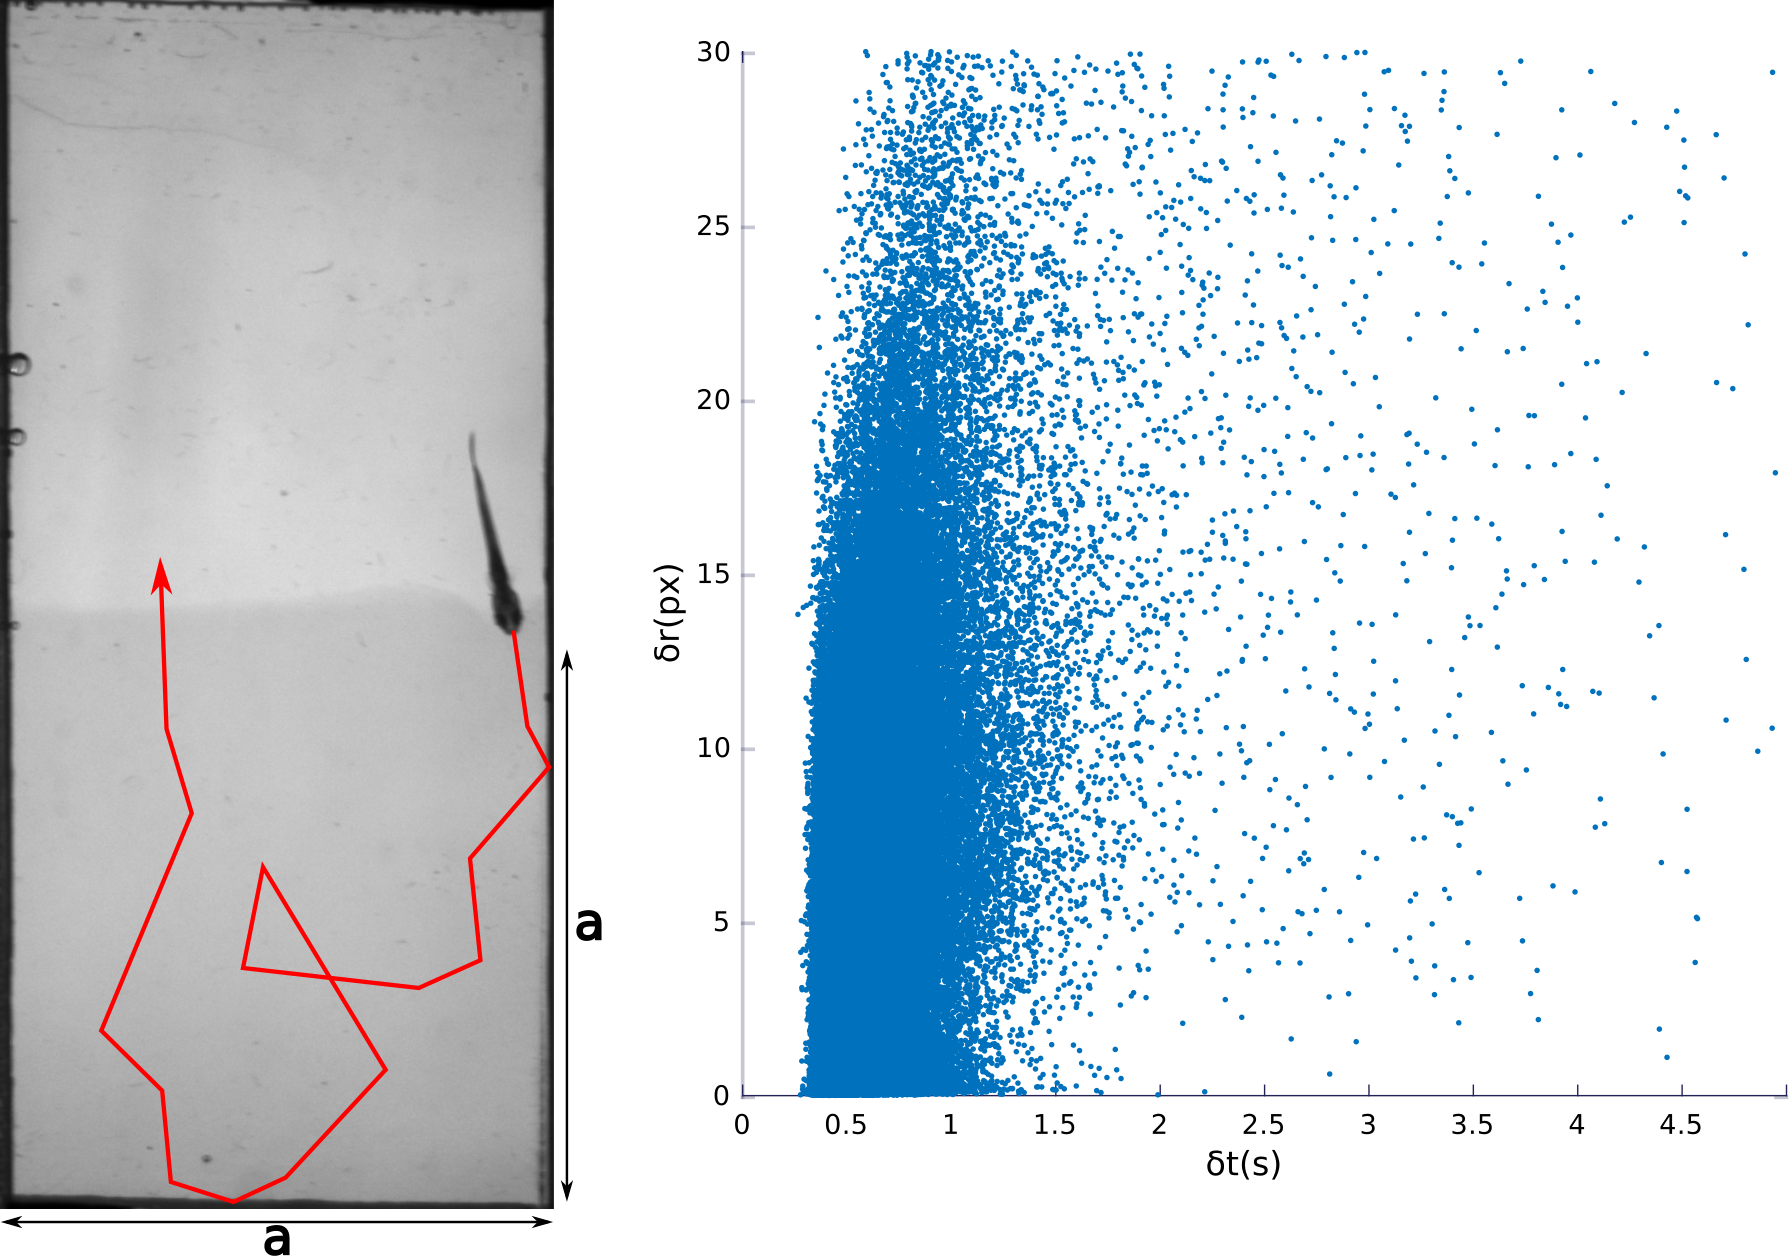
\includegraphics[width=0.75\textwidth]{part_2/assets/random_dual.png}
        \caption{\textbf{Bulk-behavior characterization} \textbf{Left} Fish trajectory inside Dual, one side is a square of size $a$ with 3 reflective walls and one absorbing wall the interface. \textbf{Right}: Correlation between $\delta t$ and $\delta r$.}
        \label{random_dual}
      \end{figure}

  The preference index can be computed as the mean time spent in the product minus the mean time spent in the buffer divided by the total time. Therefore, from Equation~\ref{eq_tmean} we expect no influence of the distribution of $\delta \theta$ in the generation of a preference index.

  In Figure~\ref{dist_time_bout}, we see no difference between the distributions when we increase the concentration in citric acid. We built a numerical simulation by generating random trajectories using the experimental distributions and computed the time-based preference index, see Figure~\ref{simu_pi}. We see that the bulk-behavior cannot explain the preference index and that decision events at the interface are crucial in generating preference.

      \begin{figure}[h!]
        \centering
        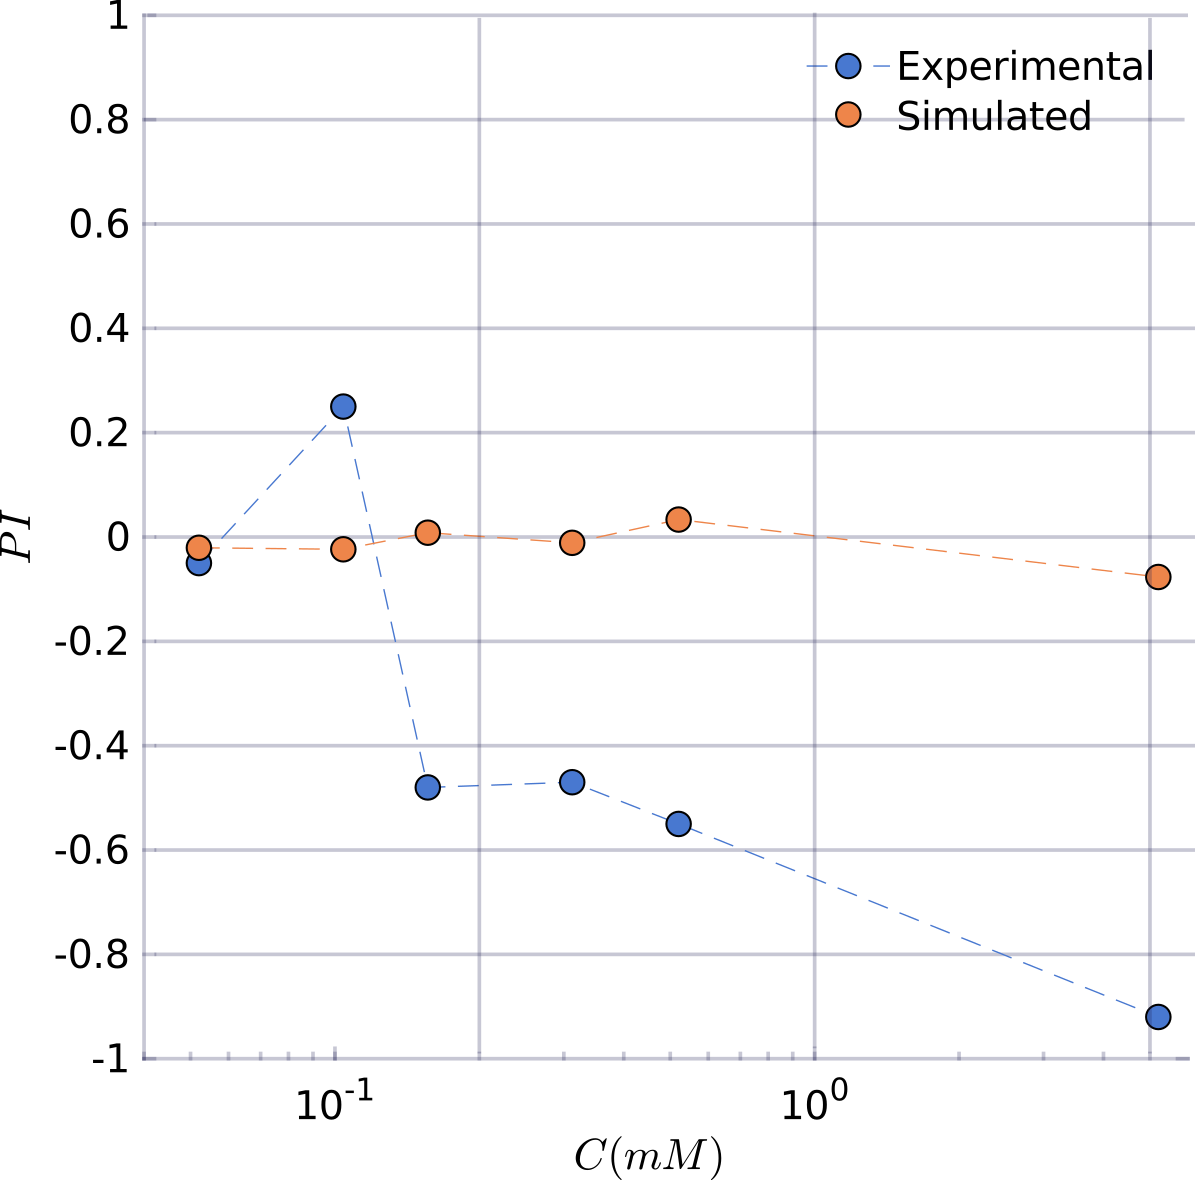
\includegraphics[width=0.75\textwidth]{part_2/assets/simu_pi.png}
        \caption{\textbf{Preference index numerical simulation}}
        \label{simu_pi}
      \end{figure}


  \paragraph{Zebrafish larvae in citric acid} Preliminary experiments were done to assess the effect of citric acid on zebrafish larvae (Figure~\ref{dist_citric_acid_lar}). Despite low statistics (see Section~\ref{discussion}) and substantial variability, we see that citric acid seems to be repulsive as expected from results with juveniles. More experiments need to be done to confirm this effect and account for the larvae variability.

    \begin{figure}[h!]
      \centering
      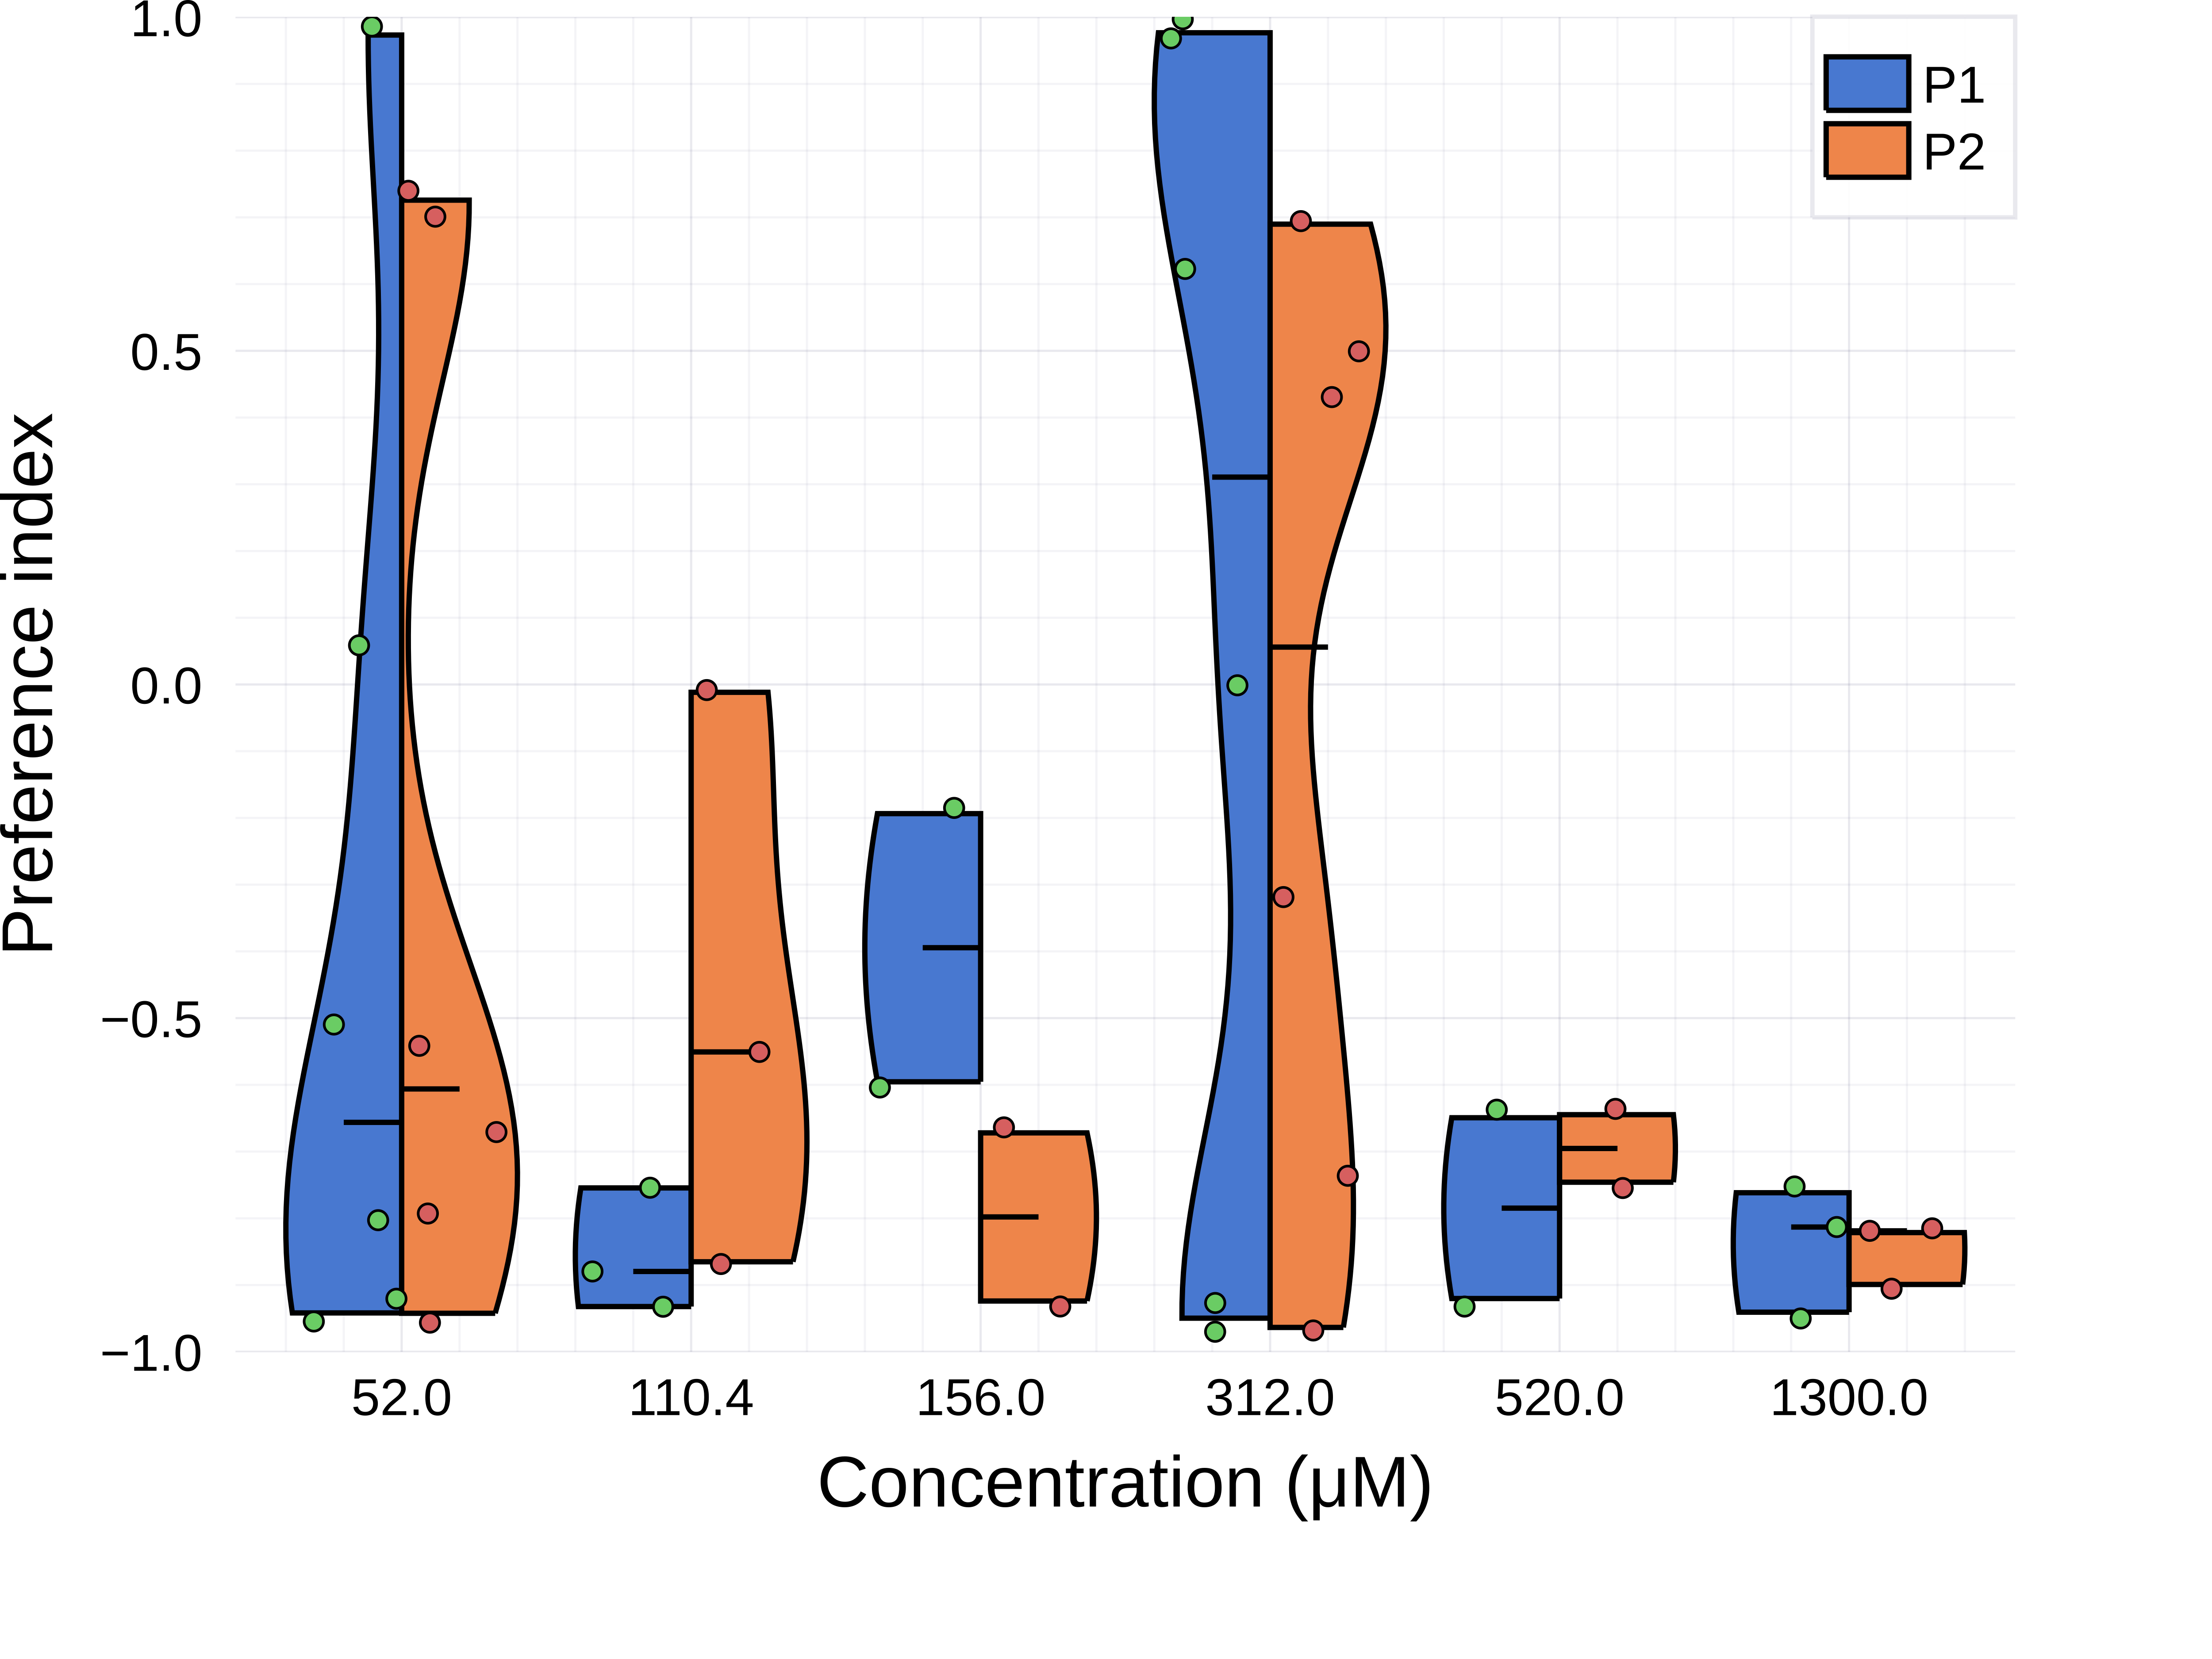
\includegraphics[width=0.75\textwidth]{part_2/assets/dist_citricacid_lar.png}
      \caption{\textbf{Citric acid: preference index for larvae} Time-based preference index, one point is one fish.}
      \label{dist_citric_acid_lar}
    \end{figure}

  Using Dual, we were able to assess the repulsion to citric acid by zebrafish. Our analysis and model were able to capture the fish behavior changes and quantify the repulsion magnitude. As expected, the inter-fish variability is large but seems to be reduced by aversion where fish adopt a stereotyped exploitation behavior.

  \paragraph{Juvenile zebrafish in quinine} Quinine is a natural alkaloid that tastes bitter, and that is a highly deterrent substance for many fish species \cite{kasumyan2003taste}. Unexpectedly, we see with the time-based preference index (Figure~\ref{dist_quinine}) that the preference seems to be mostly neutral. A slight attraction can be constated on the P1 cycle, and a neutral a slightly repulsive preference on the P2 cycle.

  Despite relatively good statistics ($\approx 7$ fish by concentration), no robust preference emerged as we see with large variability in responses.

    \begin{figure}[h!]
      \centering
      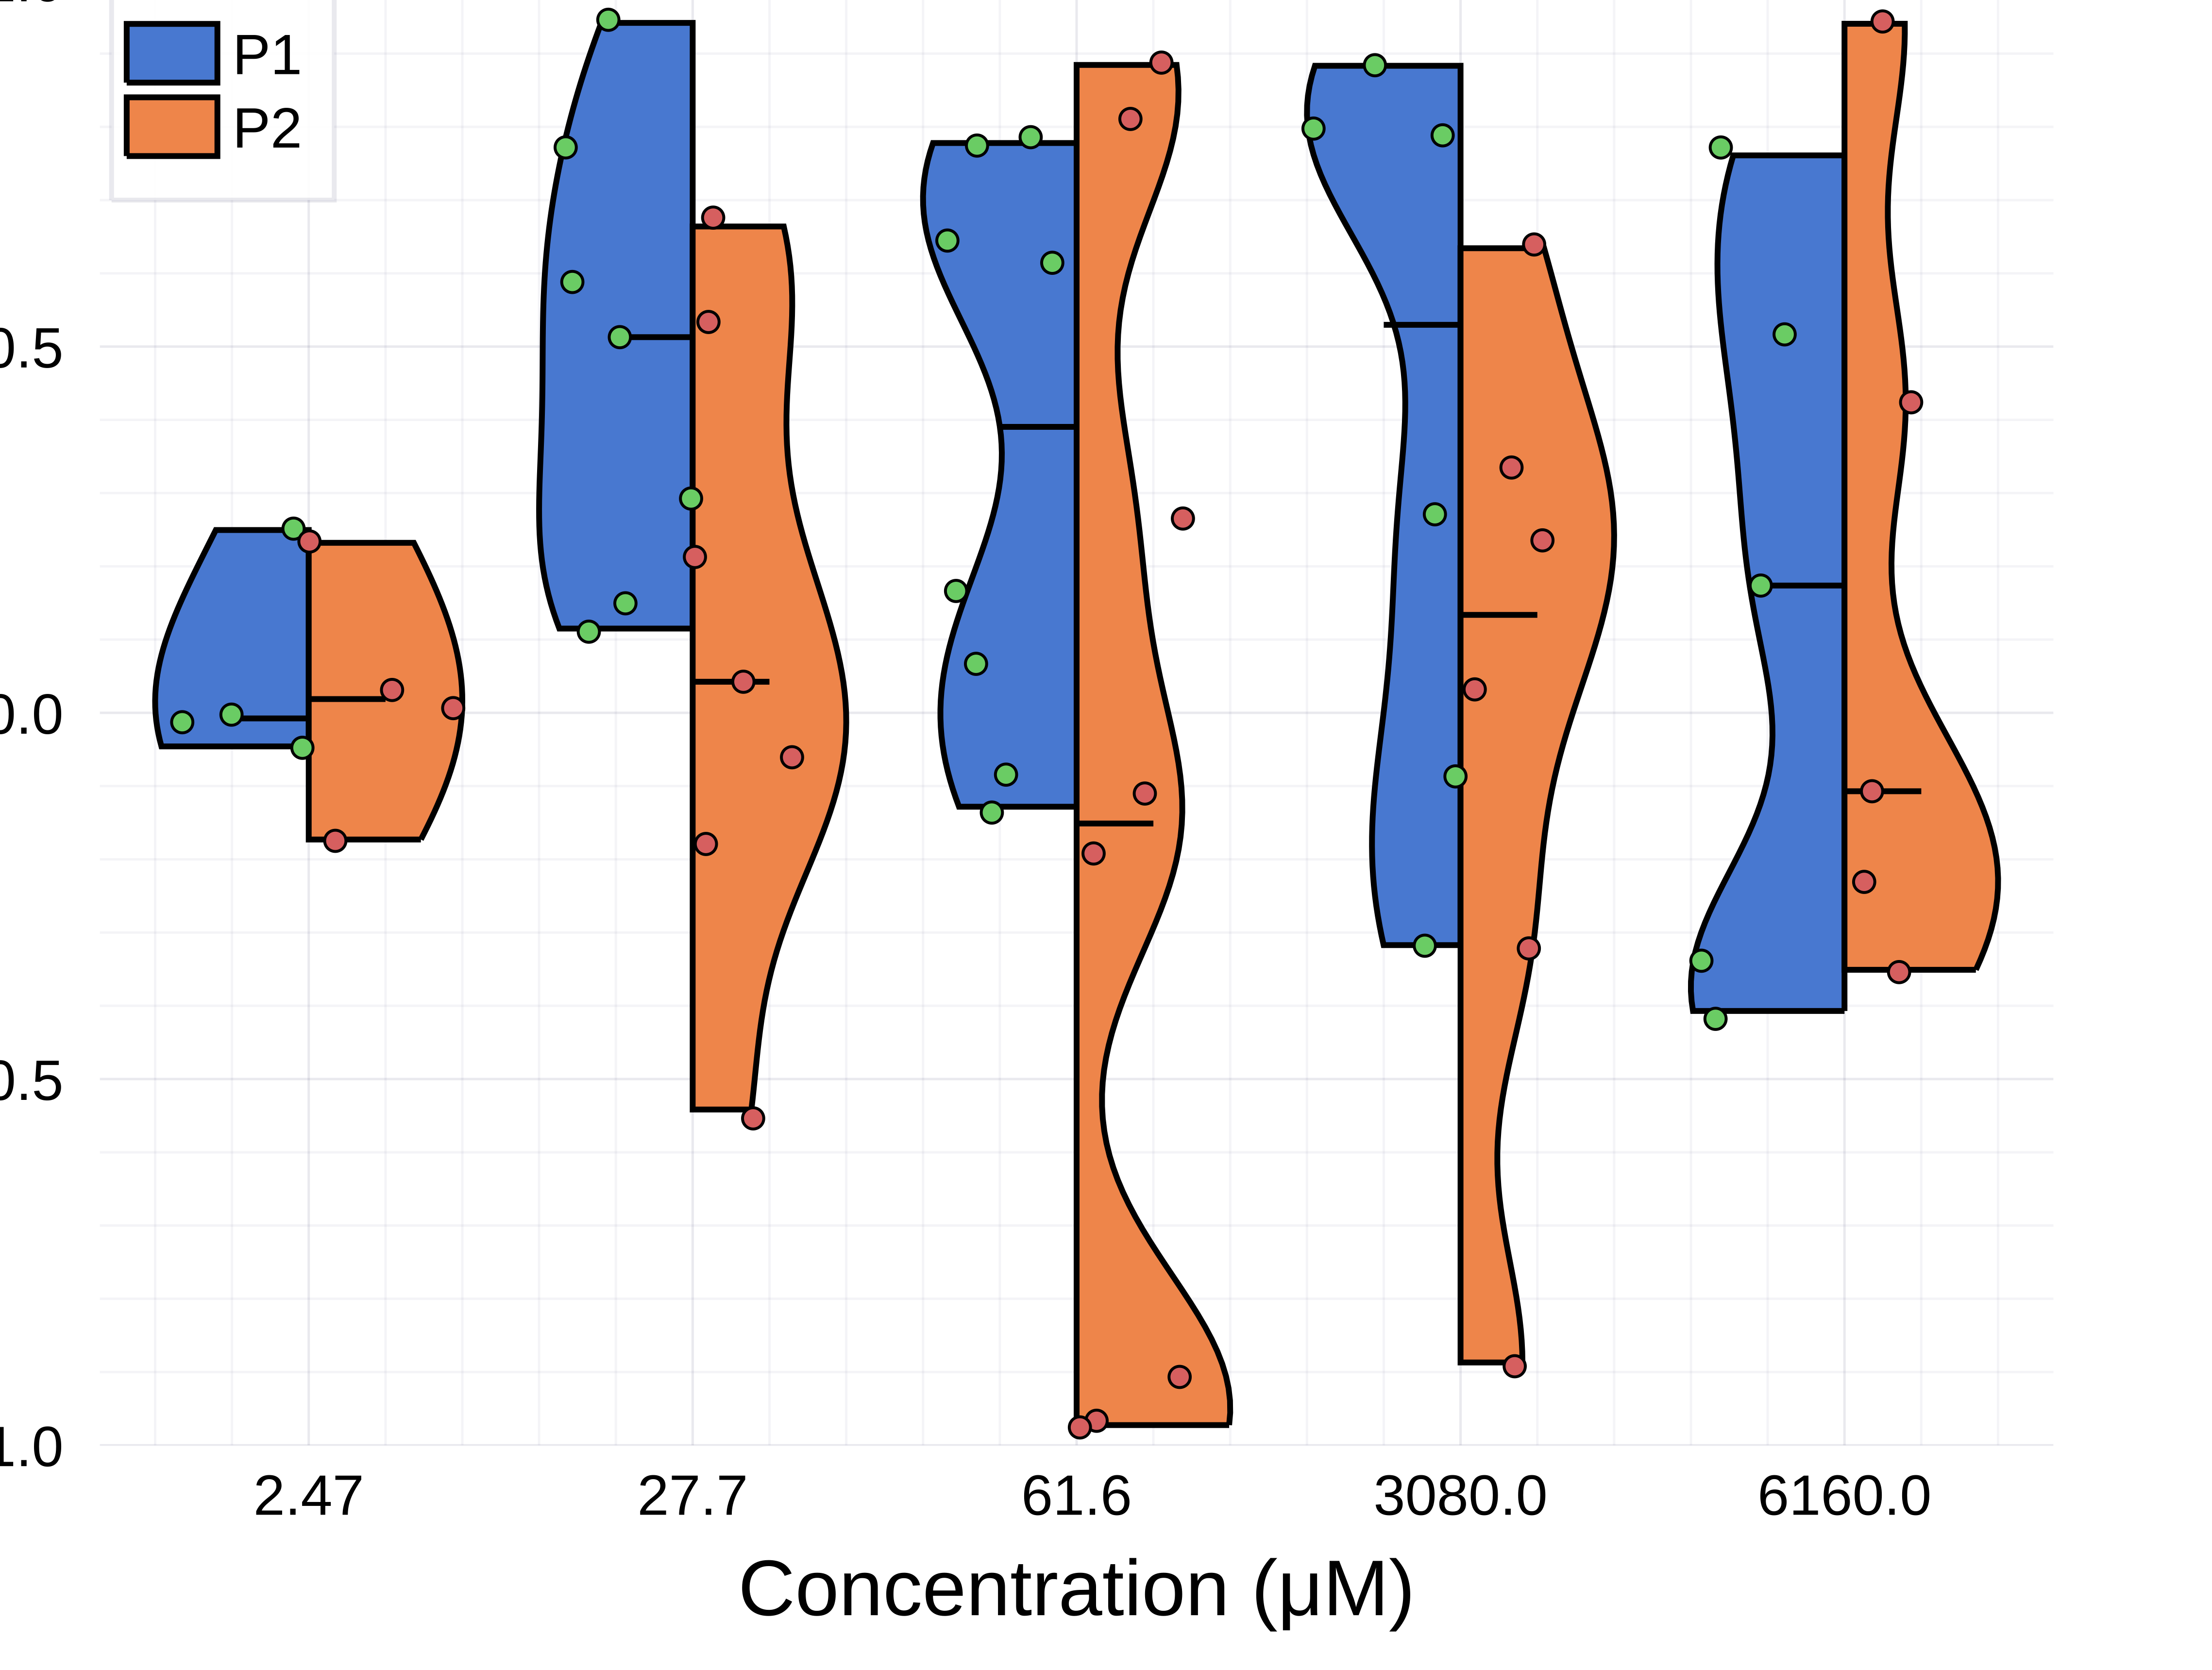
\includegraphics[width=0.75\textwidth]{part_2/assets/dist_quinine.png}
      \caption{\textbf{Quinine: preference index for juveniles} Time-based preference index. One point is one fish. }
      \label{dist_quinine}
    \end{figure}

  \paragraph{ATP and adenosine}
  Zebrafish have pear-shaped olfactory sensory neurons expressing olfactory receptors specific to adenosine \cite{wakisaka2017adenosine}. ATP, ADP, and AMP are dephosphorylated in the zebrafish olfactory epithelium \cite{wakisaka2017adenosine} and behavioral responses to adenosine and ATP were shown to exist in adults with arousal and food-seeking behavior. We assessed preference for ATP and adenosine for larval and early juvenile zebrafish. Fish were starved 24 hours before the experiment, and preference was assessed using the protocol presented above.

  \paragraph{Juvenile zebrafish in adenosine} Fish can perceive adenosine as indicated by the ratios exploration-exploitation presented in Figures~\ref{adenosine_event}~bottom and \ref{adenosine_markov}~bottom that decrease with the concentration.

  The event-based and Markov-based preference indexes (Figures~\ref{adenosine_event}~top and \ref{adenosine_markov}~top) show a slight repulsion for the P1 cycle and a slight attraction for the P2 cycle at the two lower concentrations.  The time-based preference index (Figures~\ref{adenosine}) displays a slight repulsive preference for the P1 cycle. There is no clear preference, and analysis from event-based and time-based preferences disagree, meaning that there is probably not enough statistic to conclude. Besides, the preference index distributions (Figure~\ref{dist_adenosine}) show great variability.

    \begin{figure}[h!]
      \centering
      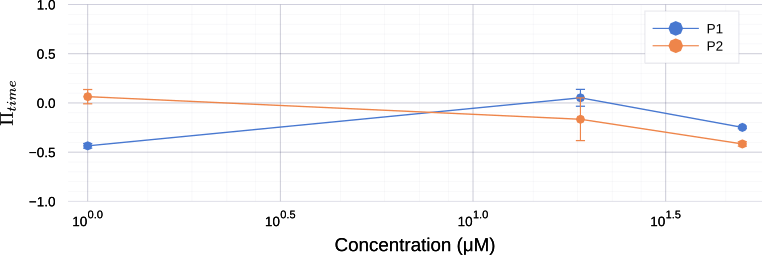
\includegraphics[width=1\textwidth]{part_2/assets/adenosine.png}
      \caption{\textbf{Adenosine: time-based preference index for juveniles} Time-based preference index (mean $\pm$ SEM, equation~\ref{mean_pi_time}).}
      \label{adenosine}
    \end{figure}

  As no clear preference emerged from the early experiments, we focused on the concentration $50 \mu M$ and increased the statistics up to $N=28$. We then saw a slight repulsion on the P1 cycle at the same level as the other concentrations. However, the P2 cycle showed a clear repulsion with a median preference index equal to $-0.6$ and 2 clusters of fish, one attracted and one repulsed.

    \begin{figure}[h!]
      \centering
      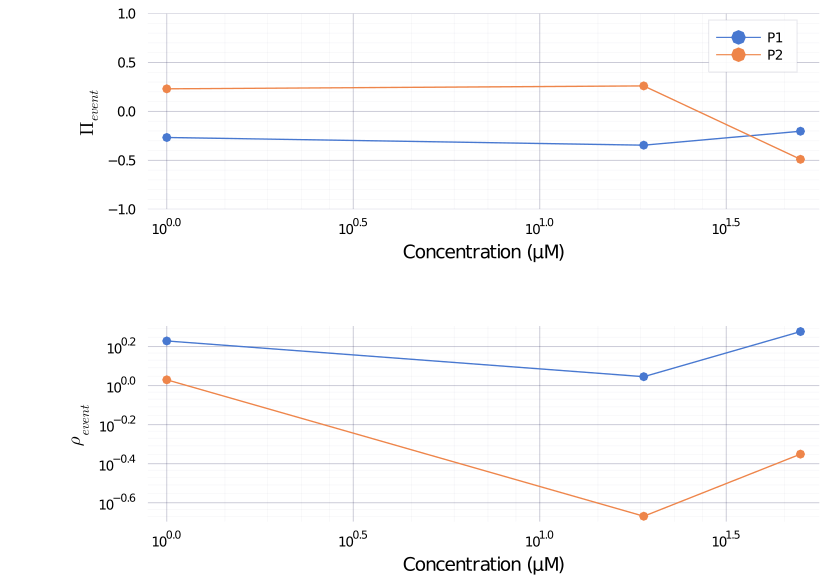
\includegraphics[width=1\textwidth]{part_2/assets/adenosine_event.png}
      \caption{\textbf{Adenosine: event-based analysis for juveniles} \textbf{Top}: Mean event-based preference index (equation~\ref{mean_pi_event}). \textbf{Bottom}: Mean ratio exploration-exploitation (equation~\ref{mean_r_event}).}
      \label{adenosine_event}
    \end{figure}

  Unexpectedly, adenosine does not seem to attract early juvenile zebrafish. On the contrary, at high concentration, it is clearly repulsive. However, one part of the fish ($\approx 30 \%$) seems to be either attracted or neutral at the second presentation of the product.

  \paragraph{Zebrafish larvae in adenosine} Zebrafish larvae were exposed to adenosine with the same protocol as juveniles. Preliminary results presented in Figure~\ref{dist_adenosine_lar} and based on the time-based preference index seem to indicate a lack of preference at all concentrations.

  \begin{figure}[h!]
      \centering
      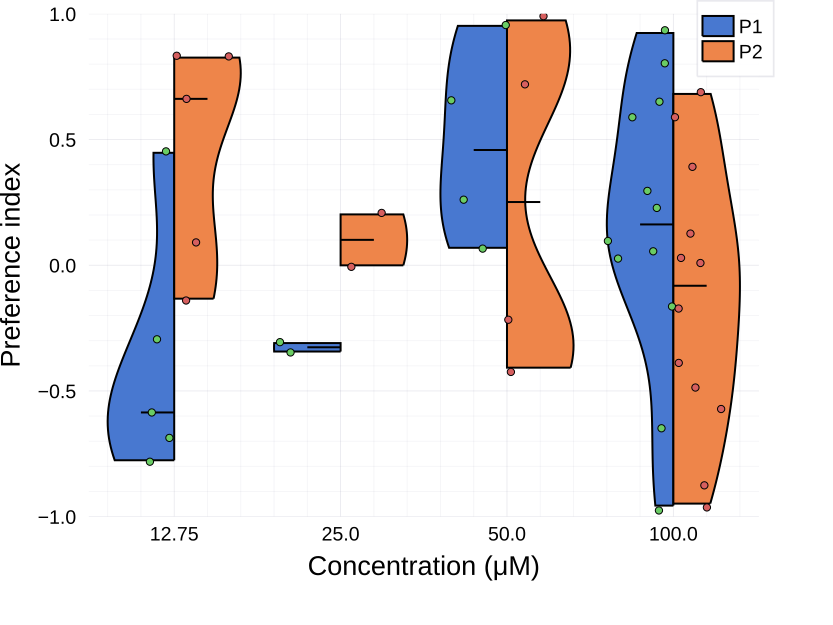
\includegraphics[width=0.75\textwidth]{part_2/assets/dist_adenosine_lar.png}
      \caption{\textbf{Adenosine: preference index for larvae} Time-based preference index. One point is one fish, black line is the distribution median.}
      \label{dist_adenosine_lar}
    \end{figure}

  \paragraph{Juvenile zebrafish in ATP} Interestingly, we found that ATP, a product that was shown to be attractive on adults, produces a two phases behavior on early juvenile zebrafish (Figures~\ref{atp}~top, \ref{atp_event}~top, and \ref{atp_markov}~top). At low concentration, the fish do not manifest a preference, but at the highest concentration ($125 \mu  M$  and $200 \mu M$), the P1 cycle is repulsive and the P2 cycle attractive.

    \begin{figure}[h!]
      \centering
      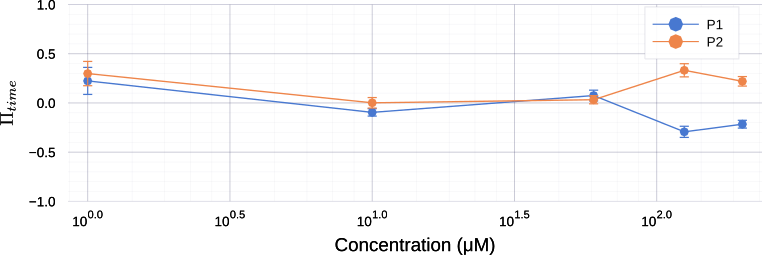
\includegraphics[width=1\textwidth]{part_2/assets/atp.png}
      \caption{\textbf{ATP: time-based preference index for juveniles} Time-based preference index (mean $\pm$ SEM, equation~\ref{mean_pi_time}).}
      \label{atp}
    \end{figure}

  Comparing the distribution of event-based, Markov-based, and time-based preference index by fish, we see that this effect is significant at $125 \mu M$ and  $200 \mu M$, see Figure~\ref{dist_atp}.

    \begin{figure}[h!]
      \centering
      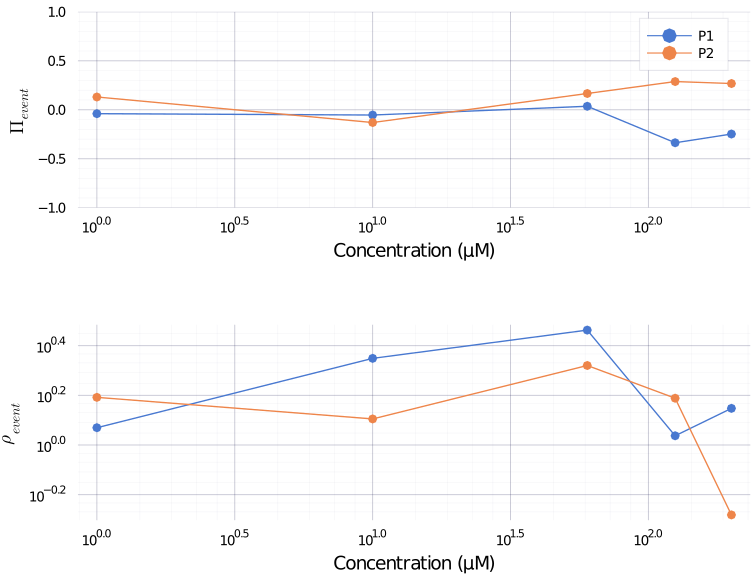
\includegraphics[width=1\textwidth]{part_2/assets/atp_event.png}
      \caption{\textbf{ATP: event-based analysis for juveniles} \textbf{Top}: Mean event-based preference index (equation~\ref{mean_pi_event}). \textbf{Bottom}: Mean ratio exploration-exploitation (equation~\ref{mean_r_event}).}
      \label{atp_event}
    \end{figure}

  A fish-by-fish analysis, see Figure~\ref{proportion}A, revealed that the fish proportion that changes its preference towards attraction increase with the concentration. Figure~\ref{proportion}B represents the $p$ and $b$ probability from the Markov chain model in function of the cycle P1 and P2. We see that many fish cross the identity line between the P1 and P2 cycle to invert their preferences.

    \begin{figure}[h!]
      \centering
      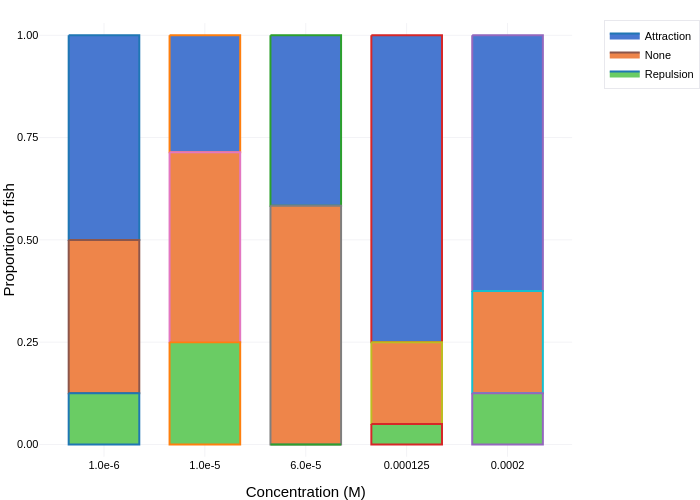
\includegraphics[width=1\textwidth]{part_2/assets/proportion.png}
      \caption{\textbf{Cycle effect} \textbf{A}. Fish proportion changing preference between the P1 and P2 cycles. \textbf{B}. Probabilities $p$ and $b$ for $125$ and $200 \mu M$, one point is one fish analyzed by one person ($2N$ fish). Cycle are represented by the point's altitude.}
      \label{proportion}
    \end{figure}

    \paragraph{Zebrafish larvae in ATP} Zebrafish larvae were exposed to ATP with the same protocol as juveniles. Preliminary results presented in Figure~\ref{dist_atp_lar} and based on the time preference index indicate a repulsion at all concentrations. High concentrations seem to produce more robust repulsive behavior with low variability.

    \begin{figure}[h!]
      \centering
      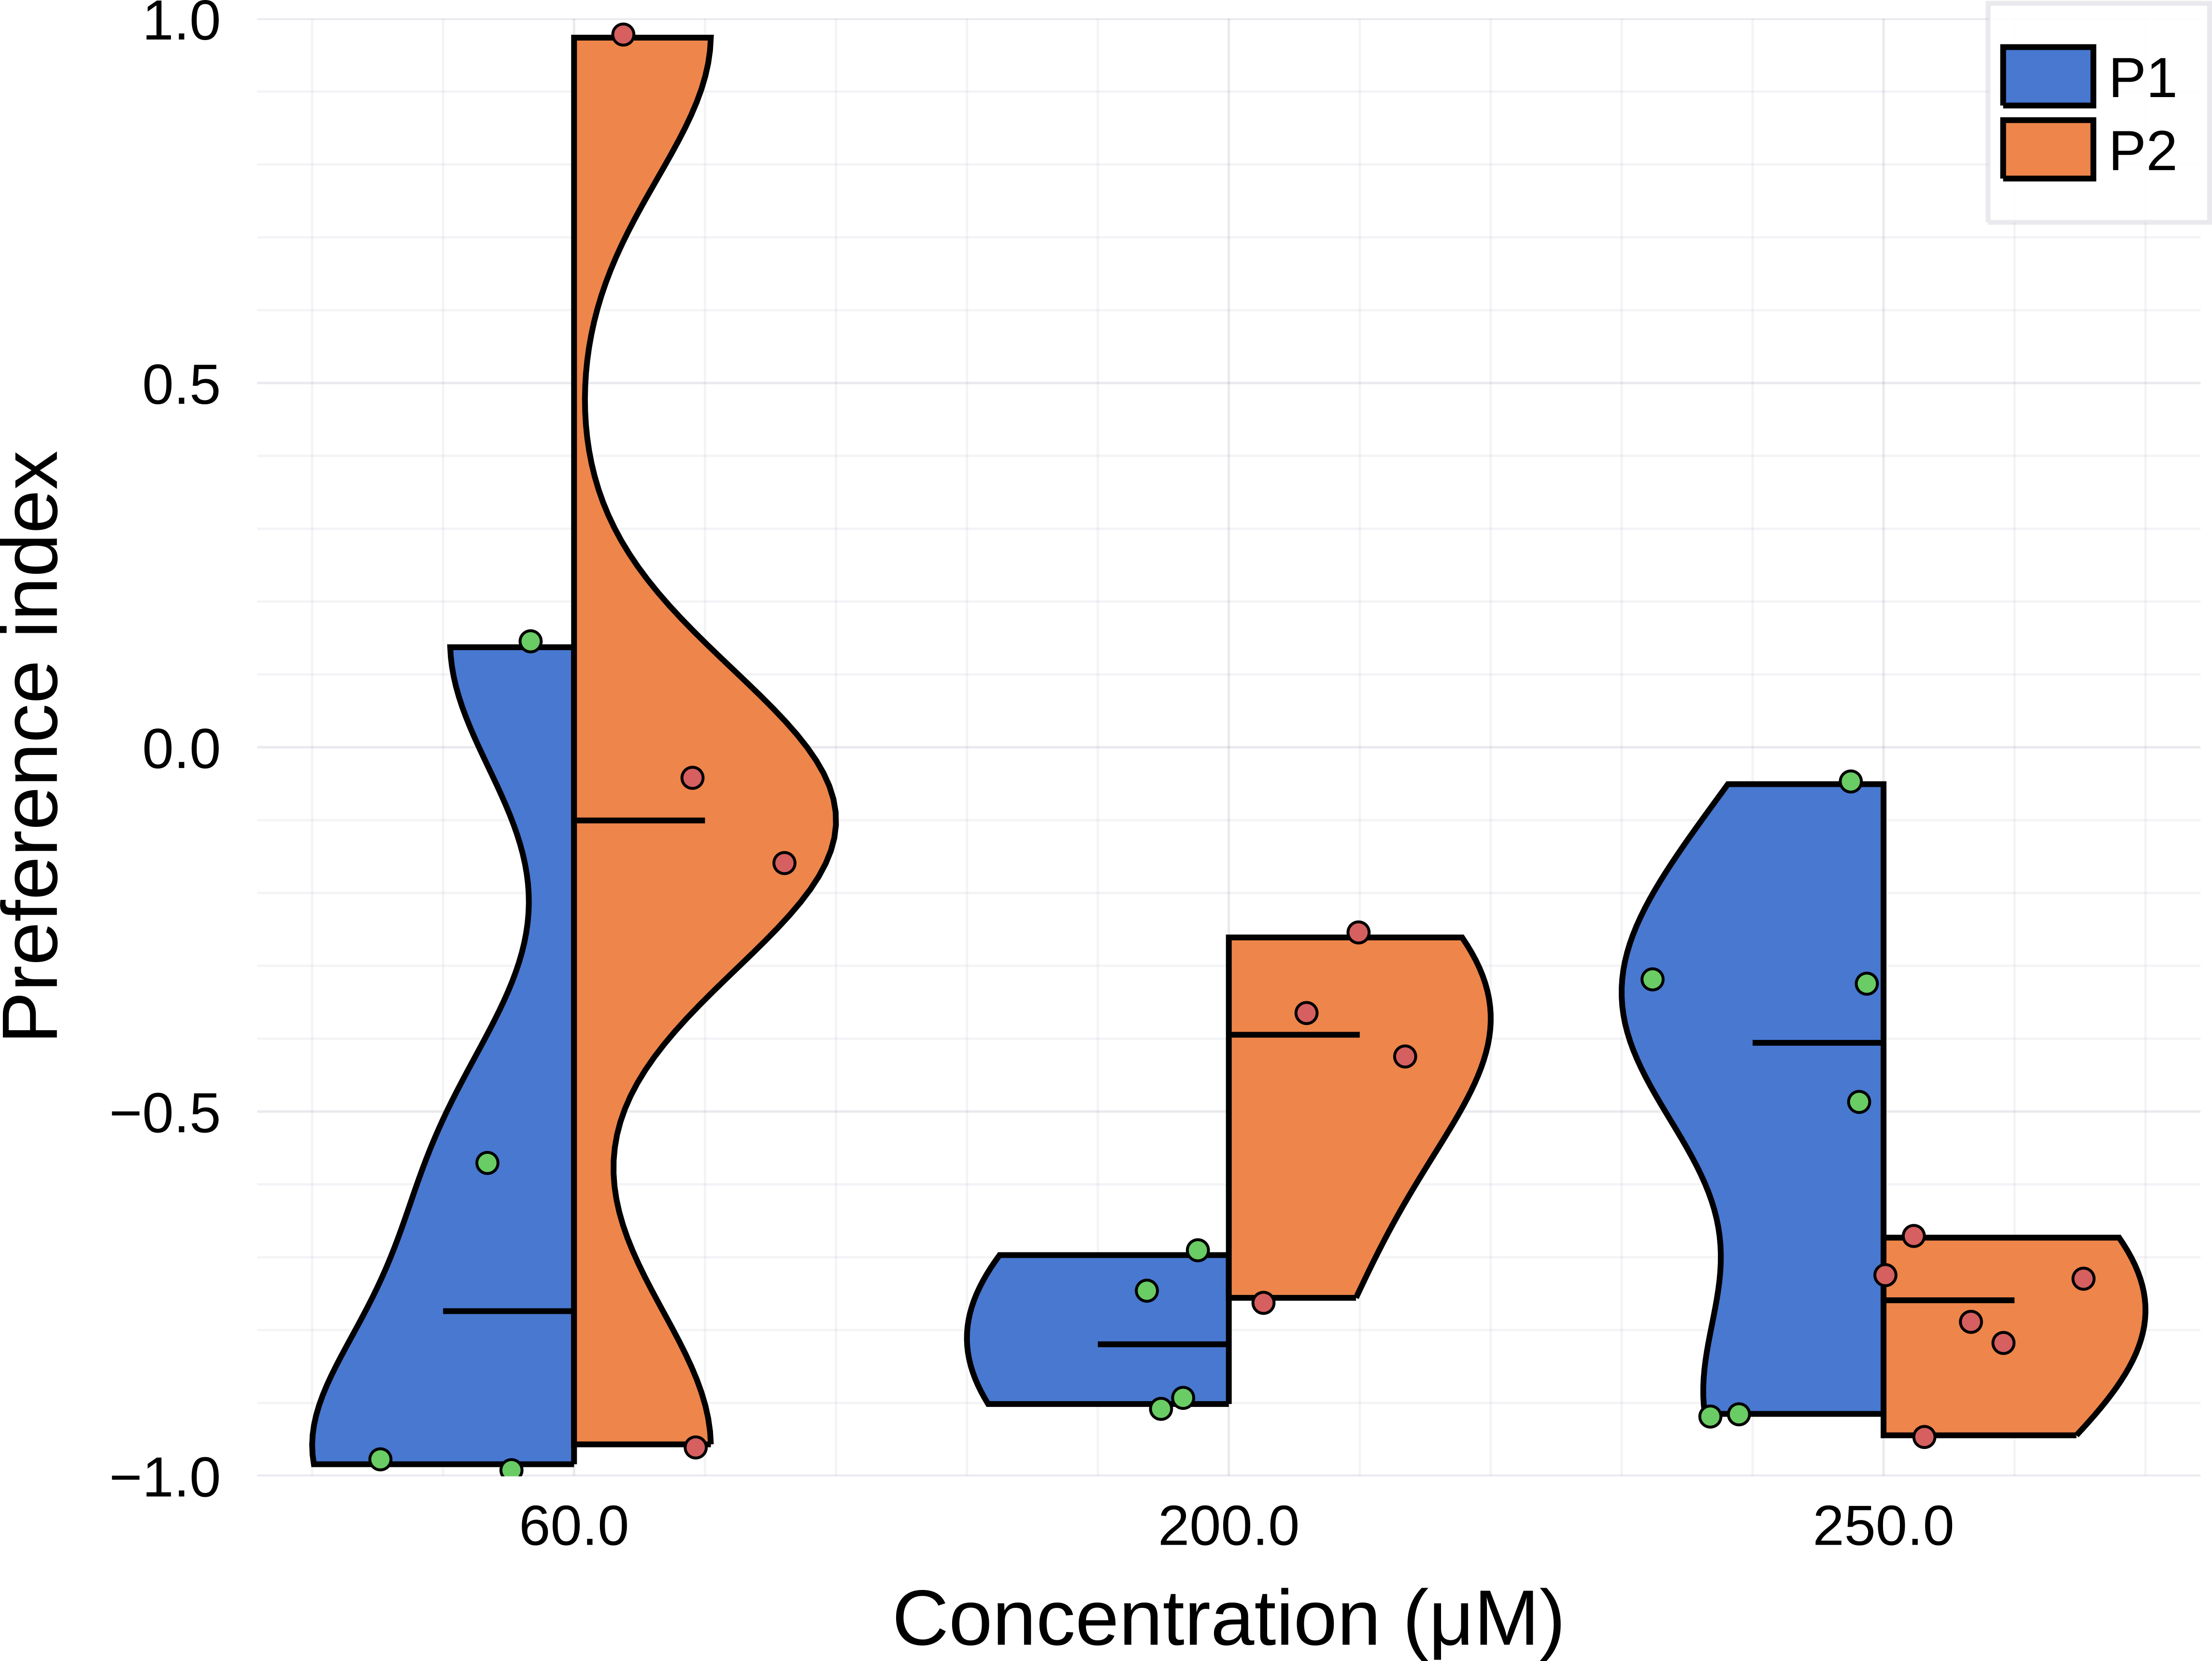
\includegraphics[width=0.75\textwidth]{part_2/assets/dist_atp_lar.png}
      \caption{\textbf{ATP: preference index for larvae} Time-based preference index. }
      \label{dist_atp_lar}
    \end{figure}

  \chapter{Discussion}
  \label{discussion}
  In these chapters, we saw how we built two experimental setups to assess and understand the chemical preference of larval and early-juveniles zebrafish.

  The Tropical River is a setup capable of producing controlled flows. The flow temperature and velocity can be precisely controlled. Turbulent and laminar jets can be created inside the flow to mimic more realistic fragmented chemical perception. This setup was initially developed to study the chemically-driven navigation after finding a robust, attractive compound with Dual. Finding such a product was challenging because it requires many statistics, thus many experiments. We have concentrated our efforts on this task with Dual; therefore, we could not use The Tropical River in this project's context. Nonetheless, several preliminary experiments were performed to check the setup. It was used in another project by Bill François to study fish swimming taking advantage of the flow velocity control and high framerate imaging.

  Dual is a high-throughput chemical screening setup with a high level of versatility that allows testing several combinations of products, concentrations, and fish ages easily and rapidly. The setup is scalable and can be built at the laboratory for less than 2 000 euros. In the first part of the thesis, we built the setup and controlled that it did not have any bias. We also checked that the infrared dye used to visualize the flow was neutral to the fish.

  Then we developed several analysis methods to capture the fish preference and behavior. These methods are fragmented according to fish ages and products. We first implemented a coarse-grained approach where we recorded the fish's position and computed the time-based preference index taking the median interface position. Then we tried to refine this approach to better characterize the fish behavior at the interface by extracting the interface position. This was not practically achievable due to several constraints: time, fish complex behavior, and challenging image processing problems on a large amount of data (8 To of data). Finally, we chose to perform a manual analysis that focuses on events happening at the interface, moments where the fish had to make a decision. It was possible to confirm the time-based analysis results with this approach and characterize the fish behavior more precisely. This method was only applied to products with enough statistics and already interesting effects to delve into.

  We successfully used Dual to assess the chemical preference of several products. We show a strong aversion to citric acid and an exciting effect with ATP where fish inverts their preferences at the second product presentation.

  Adults were shown to be attracted by ATP without mention of prior exposures. Our results tend to suggest that larvae are repulsed and juveniles repulsed then attracted in a second exposition to ATP. This behavior is probably more complicated because we see variability among fish, with fish changing preference and others not. Work remains to be done to precisely characterize this effect. It would be interesting to study the proportion of fish switching preference by, for example, forcing ATP on both sides for a given duration and then check preference as a function of the first presentation time or the first presentation concentration. An interesting question would be to check what happened at the third presentation of ATP. All these experiments can be done easily by modifying the protocol in Dual. If this attractive preference persists in time, ATP could be used in The Tropical River to study chemically-driven navigation. A temporal characterization would also be of great interest. Studying the effect at a fixed concentration, like $125 \mu M$, and varying the fish age. It would help understand the development of ATP's perception from larval to adult stage.

  Preliminary results shown with larvae need more statistics. Studying larvae poses several challenges. First, larvae tend to explore less than juveniles, and combined with their small sizes, they do not frequently cross the interface. We circumvented this problem by putting up to 4 larvae by experiment, thus increasing the statistics, but this adds work in the analysis phase. Secondly, larvae are more susceptible to fatigue and freezing than juveniles. It frequently happens that larvae stop swimming and do not recover until the end of the experiment.
For this reason, assessing the ATP effect on larvae is very challenging: reducing cycle length to reduce fatigue would lead to fewer crossing events, but longer cycles would lead to more fish dropouts before the second cycle. Another solution would be to reduce the chamber size to increase crossing events with the same cycle length. For all these reasons, studying larvae would need many statistics, which we had not the time to do in this thesis.

  Studying the chemical perception of zebrafish proved to be challenging. The fish inter-variability is high, as we have seen by screening products. In these experiments, we use four Duals to record up to 350 hours of usable experiments, but we see that more statistics are needed. We hope that Dual as a low-cost, easily replicable setup will encourage people to build and use the setup to better characterize zebrafish chemo-preference.


\begin{appendices}

  \chapter{Dual bill of materials}
  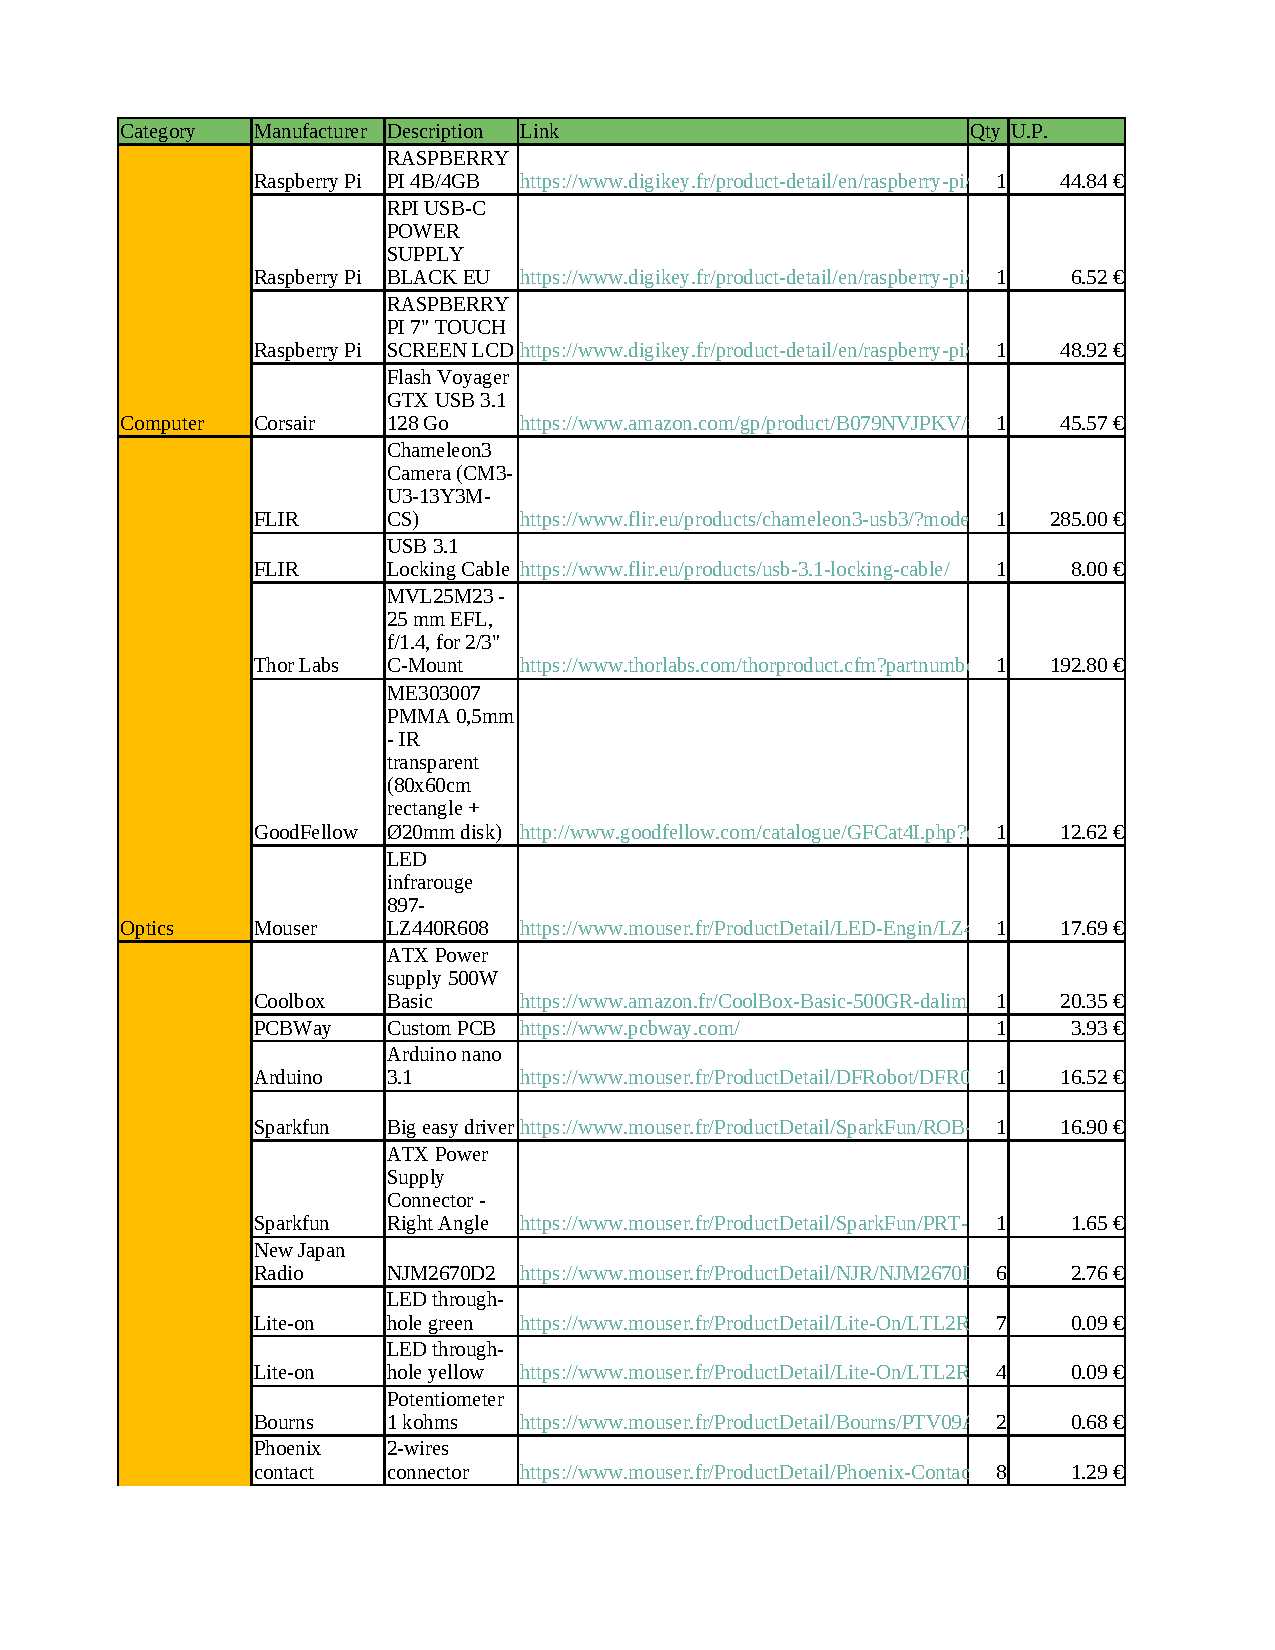
\includepdf[pages=-]{part_2/assets/bom.pdf}
  \label{bom}

  \chapter{Touch-and-turn behavior}
    \label{touch-and-turn}
    Strong preferences are always found in a regime where exploitation dominate. It can be easily observed by a behavior that we call touch-and-turn, see Figure~\ref{touchandturn}. The fish goes to the interface to sense it, then abruptly turns to return to its preferred side.

      \begin{figure}[h]
        \centering
        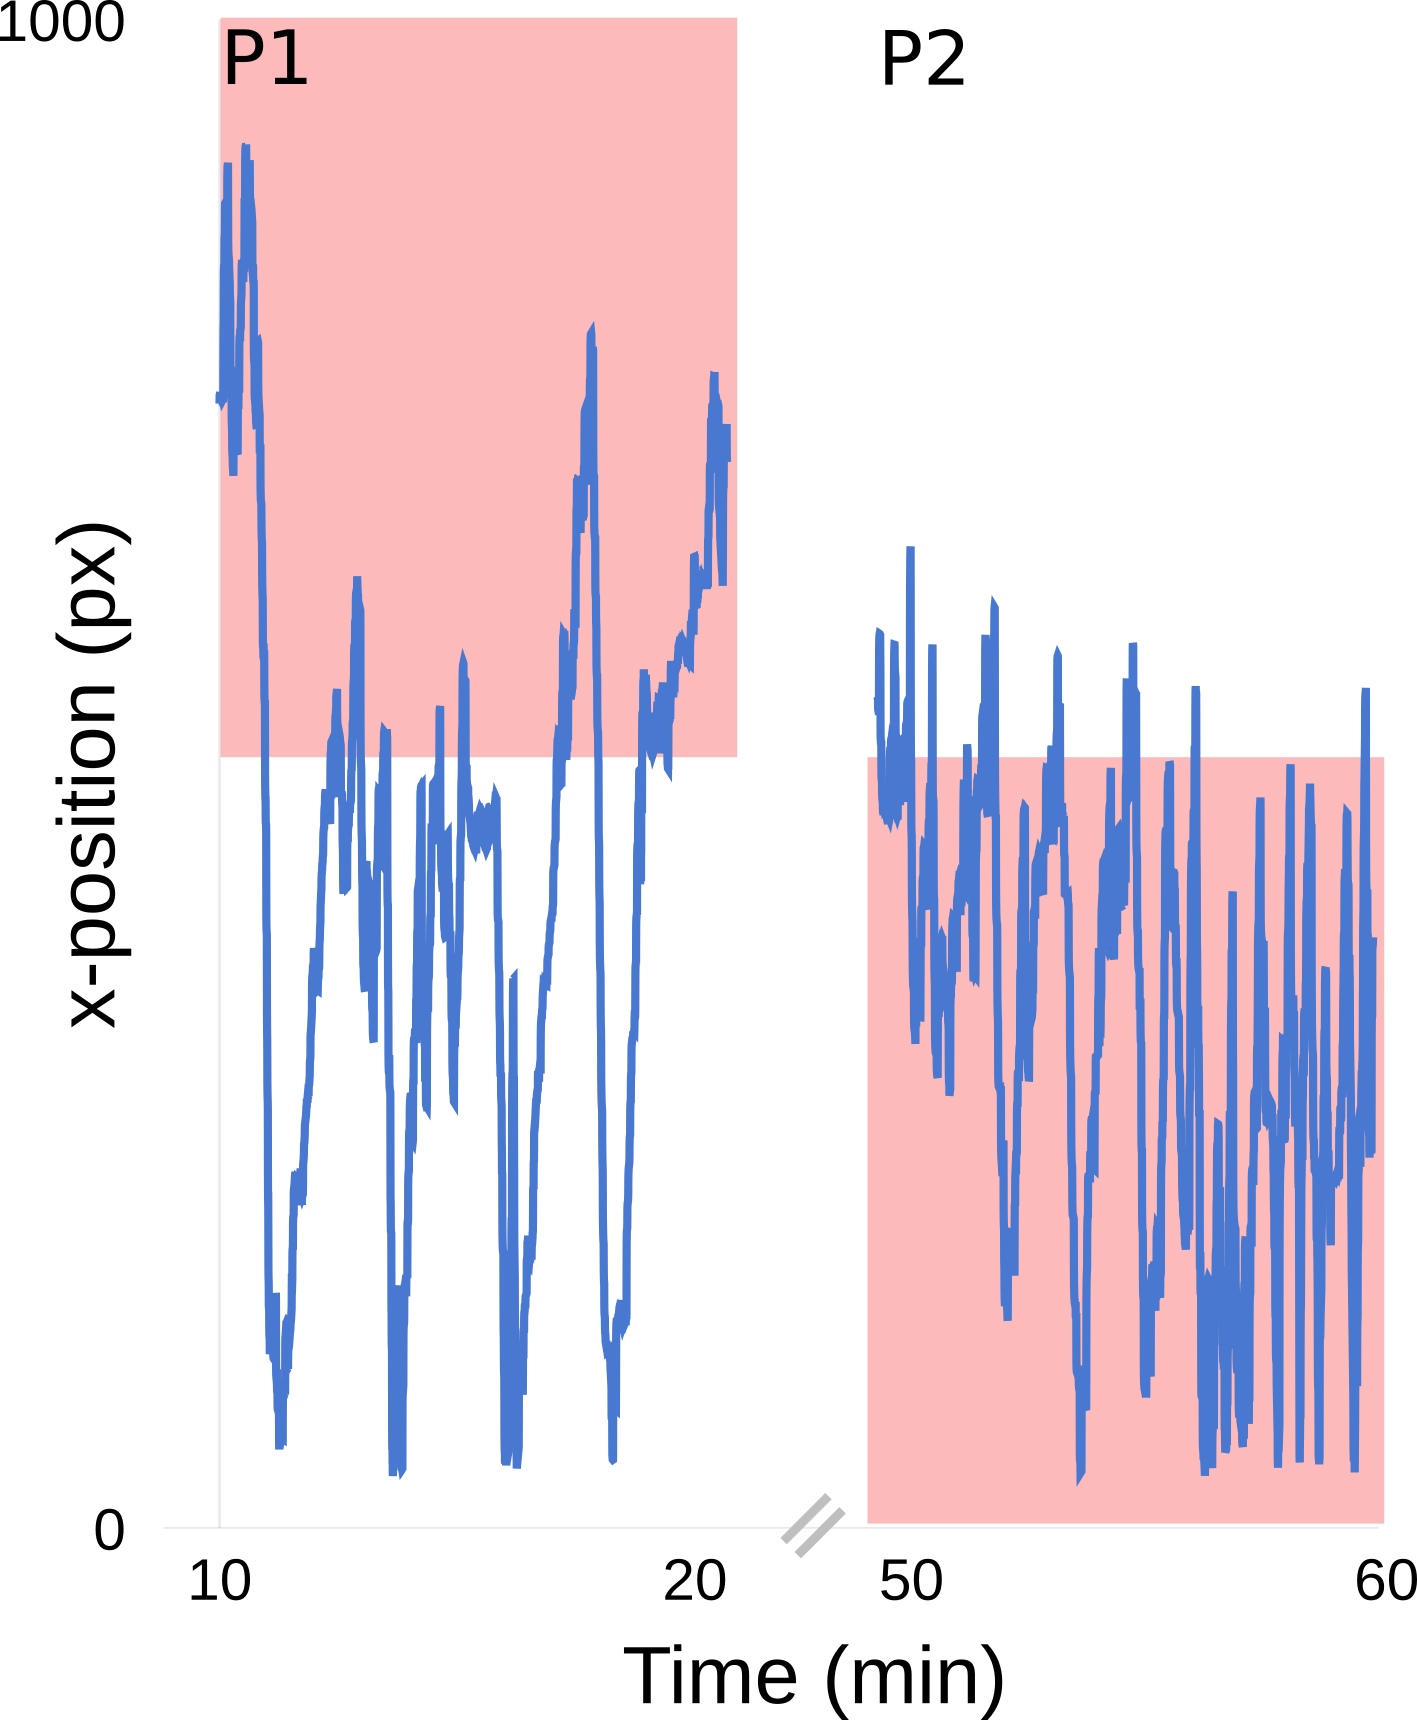
\includegraphics[width=0.5\textwidth]{part_2/assets/trace.png}
        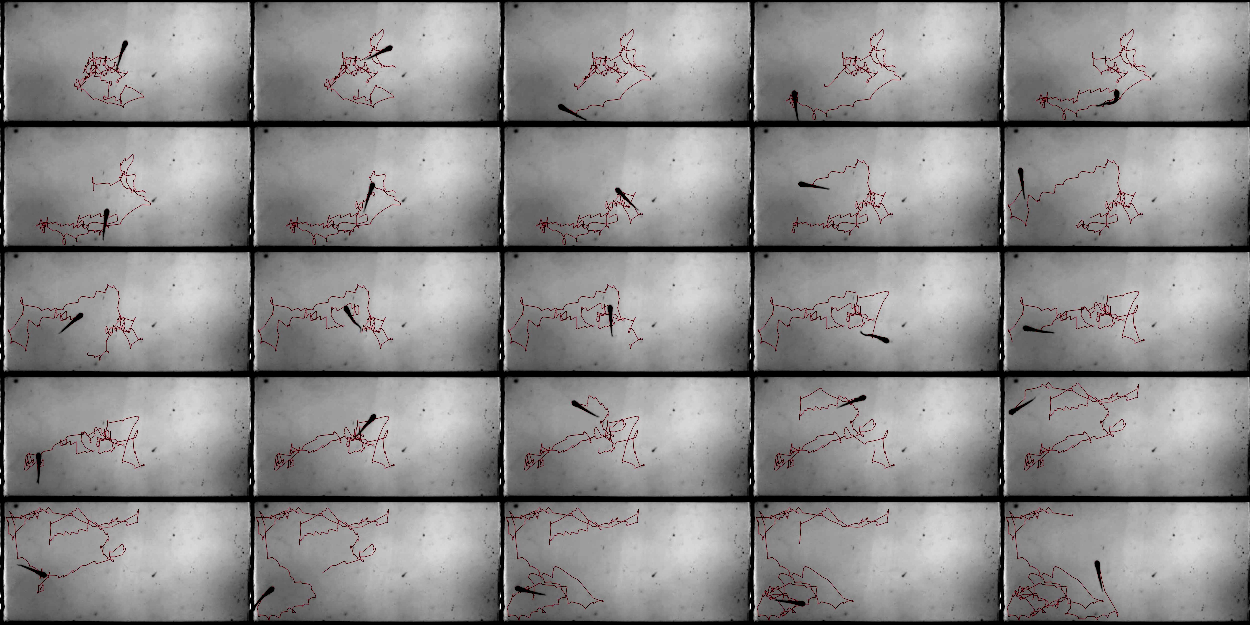
\includegraphics[width=0.8\textwidth]{part_2/assets/ret.png}
        \caption{\textbf{Touch-and-turn behavior} \textbf{Left}: Fish trajectory in $200 \mu M$ of ATP (red box).}
        \label{touchandturn}
      \end{figure}


  \chapter{Calculation}
   \label{mean_quantities}
    \section{Mean quantities}
    Mean quantities were calculated from events count following these definition:
    \begin{equation}
      \overline{\Pi_{time}} = \frac{\sum_{fish}^{}(\Pi_{time})}{N_{fish}}
      \label{mean_pi_time}
    \end{equation}
    \begin{equation}
      \overline{\Pi_{event}} = \frac{\sum_{fish}^{}(n_{BP} + n_{PP} - n_{BB} - n_{PB})}{\sum_{fish}^{}(n_{BP} + n_{PP} + n_{BB} + n_{PB})}
      \label{mean_pi_event}
    \end{equation}
    \begin{equation}
      \overline{\rho_{event}} =\frac{\sum_{fish}^{}(n_{BP} + n_{PB})}{\sum_{fish}^{}(n_{BB} + n_{PP})}
      \label{mean_r_event}
    \end{equation}
    \begin{equation}
      \overline{p} = \frac{\sum_{fish}^{}n_{BP}}{\sum_{fish}^{}(n_{BP} + n_{BB})}
    \end{equation}
    \begin{equation}
      \overline{b} = \frac{\sum_{fish}^{}n_{PB}}{\sum_{fish}^{}(n_{PB} + n_{PP})}
    \end{equation}
    \begin{equation}
      \overline{\Pi_{Markov}} = \bar{p} - \bar{b}
      \label{mean_pi_markov}
    \end{equation}
    \begin{equation}
      \overline{\rho_{Markov}} = 2Min(\bar{p}, \bar{b}) - 1
      \label{mean_r_markov}
    \end{equation}

    \section{Statistical tests}
    Statistical significance was evaluated using the Wilcoxon signed-rank test, one-sided when knowing the effect's direction, or two-sided otherwise. In the case of the event-based analysis, the test was carried out separately on the two independent manual counting then averaged to avoid a size effect bias.

    \section{Image analysis}
     \label{auto_analysis}
    Fish head position was extracted using FastTrack. Each recording was manually checked to remove low-quality movies either with imperfect flows or non-responsive fish. Swim-bouts were extracted using the velocity signal and a threshold.

    A custom image processing procedure was developed to extract the interface using the contrast difference due to the dye \footnote{\url{https://github.com/LJPZebra/dual_analysis/tree/master/dual_cli}}. First, the maximal and minimal z-projection of the movie was calculated. For the minimal projection, the fish is masked with a white mask on each image before the projection, only keeping the flow and not projection the fish. Each image of the movie is then normalized with minimal and maximal projection. Finally, the interface was detected using an Otsu threshold.

    A python command-line interface \footnote{\url{https://github.com/LJPZebra/dual_analysis}} was created to export the relevant data in a synthetic toml file easy exportable, one experiment by file. Statistical analysis and numerical simulations were performed using Python and Julia programming language.

  \chapter{Kinematic parameter distributions}
    \begin{figure}[h!]
      \centering
      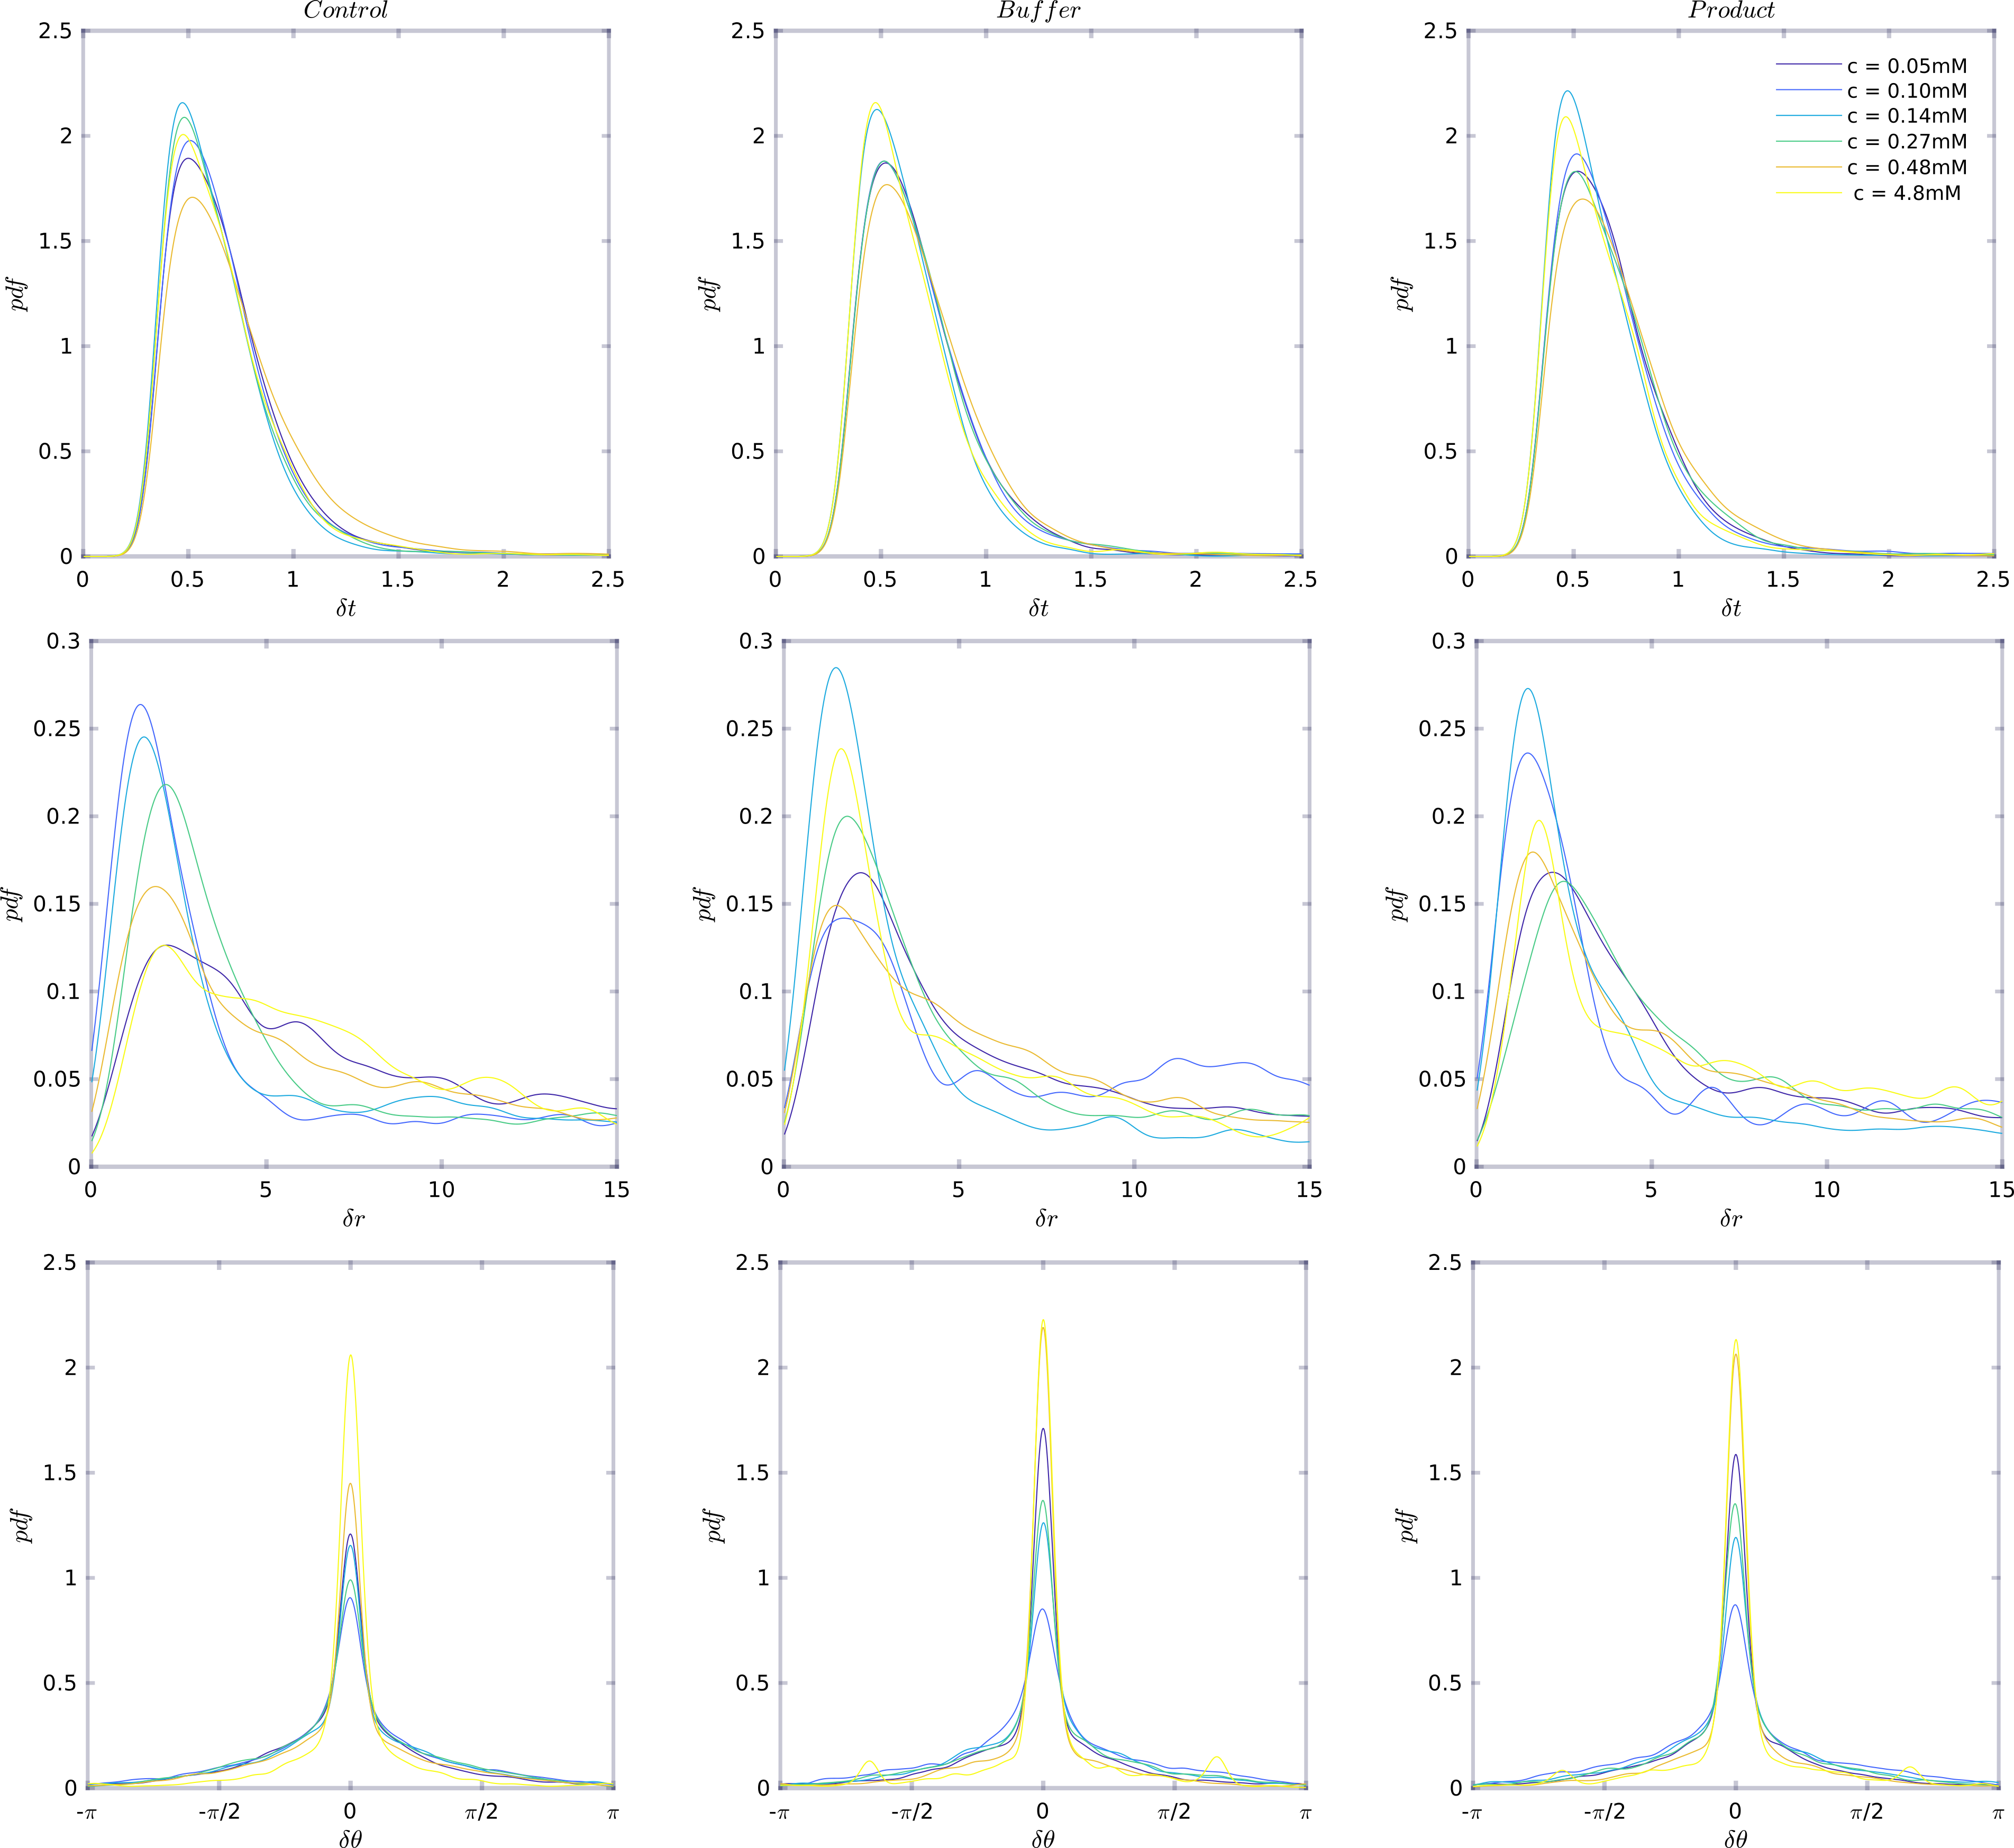
\includegraphics[width=1\textwidth]{part_2/assets/dist_citric_random.png}
      \caption{\textbf{Distributions of kinematic parameters for juveniles in citric acid.} \textbf{Top}: $\delta t$ time between on the onset of successive bouts. \textbf{Middle}: $\delta r$ distance between on the onset of successive bouts. \textbf{Bottom}: $\delta \theta$ angle between on the onset of successive bouts. Control means kinematic parameters extracted from the B1 cycle, buffer (resp. product) are extracted from P1 and P2 cycles when the fish is in the buffer (resp. product).}
      \label{dist_time_bout}:
    \end{figure}

  \chapter{Markov model results}
    \begin{figure}[h]
      \centering
      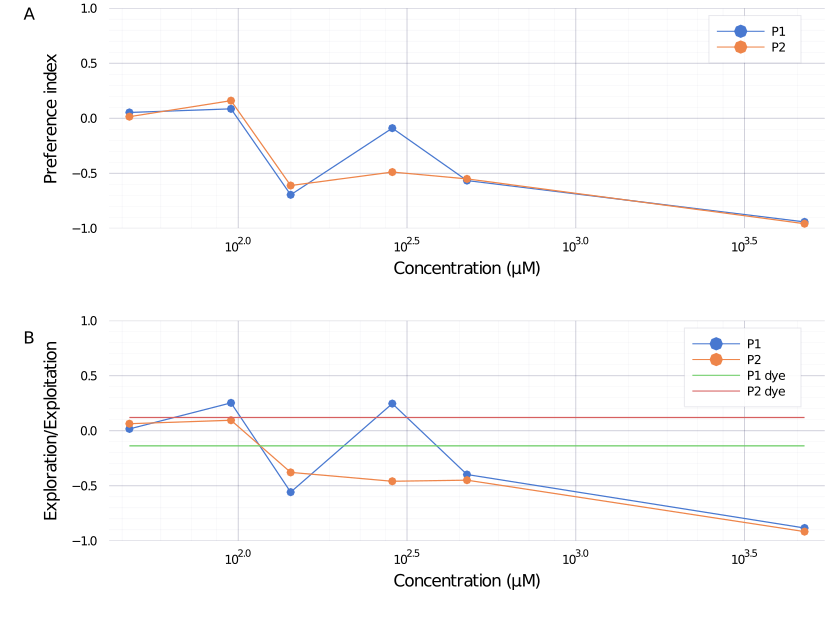
\includegraphics[width=0.8\textwidth]{part_2/assets/citricacid_markov.png}
      \caption{\textbf{Citric acid: Markov chain analysis for juveniles} \textbf{Top}: Mean Markov-based preference index (equation~\ref{mean_pi_markov}). \textbf{Bottom}: Mean Markov ratio exploration-exploitation (equation~\ref{mean_r_markov}).}
      \label{citric_acid_markov}
    \end{figure}
    \begin{figure}[h]
      \centering
      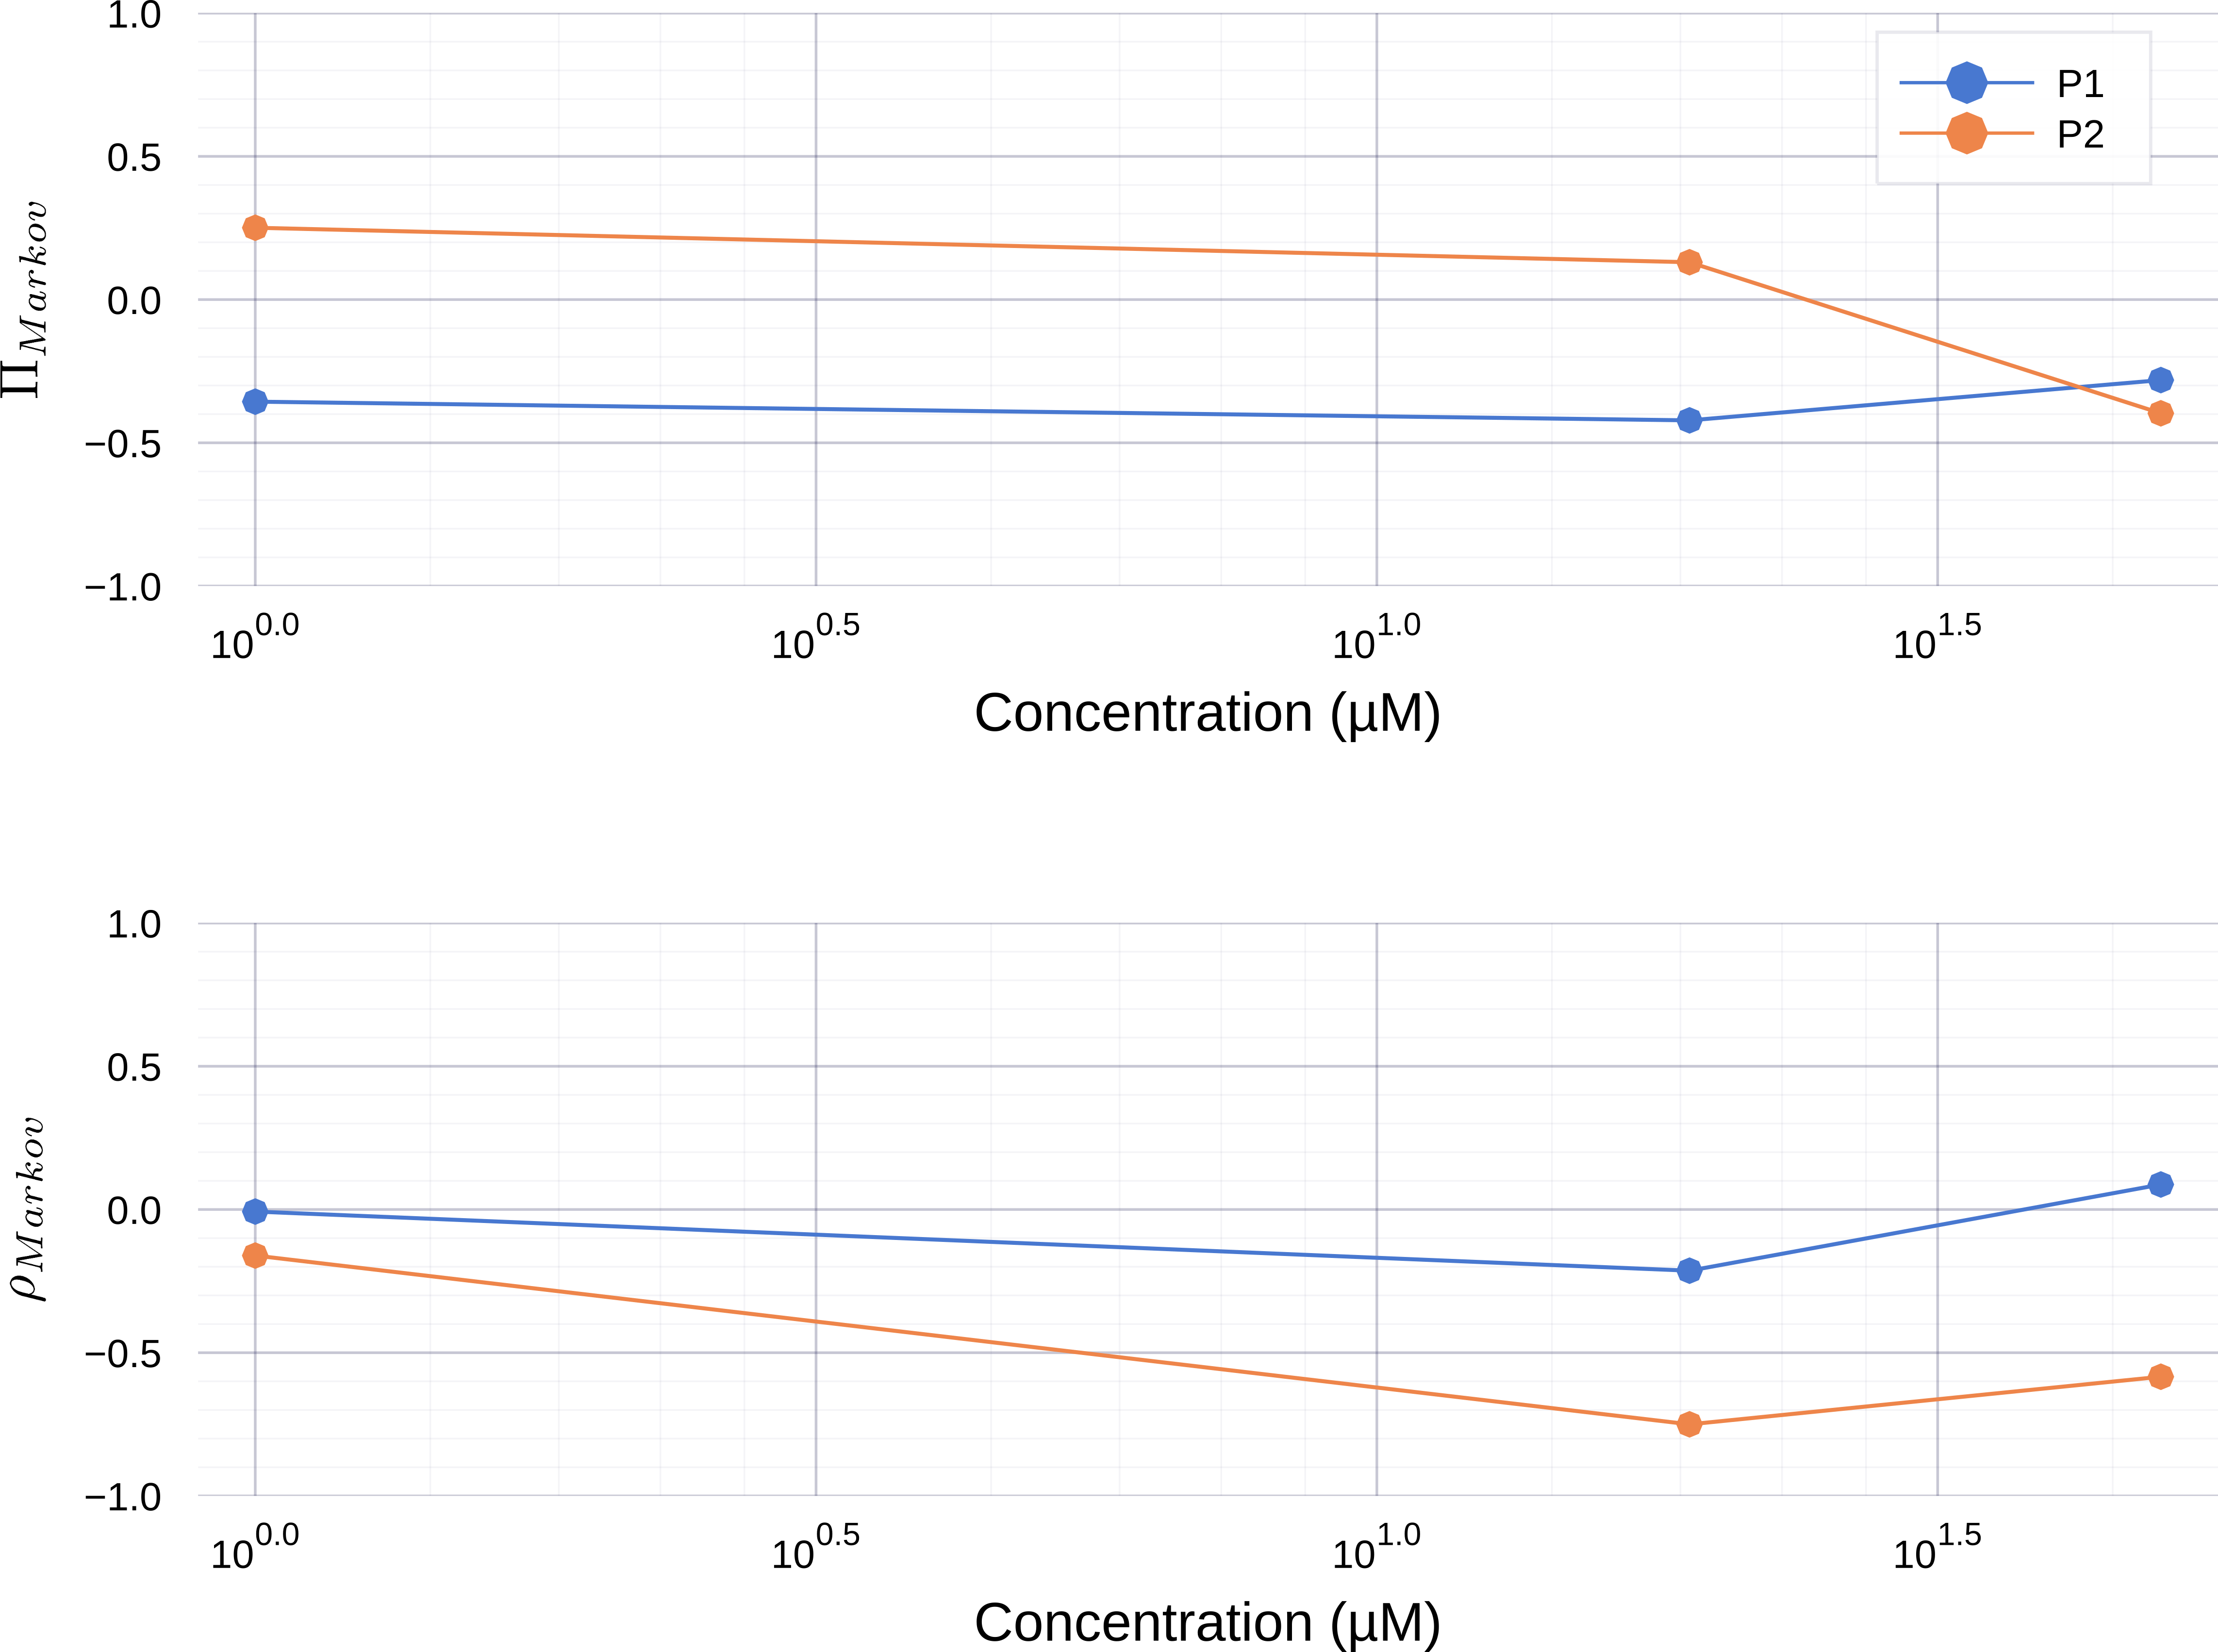
\includegraphics[width=0.8\textwidth]{part_2/assets/adenosine_markov.png}
      \caption{\textbf{Adenosine: Markov chain analysis for juveniles} \textbf{Top}: Mean Markov-based preference index (equation~\ref{mean_pi_markov}). \textbf{Bottom}: Mean Markov ratio exploration-exploitation (equation~\ref{mean_r_markov}).}
      \label{adenosine_markov}
    \end{figure}
    \begin{figure}[h]
      \centering
      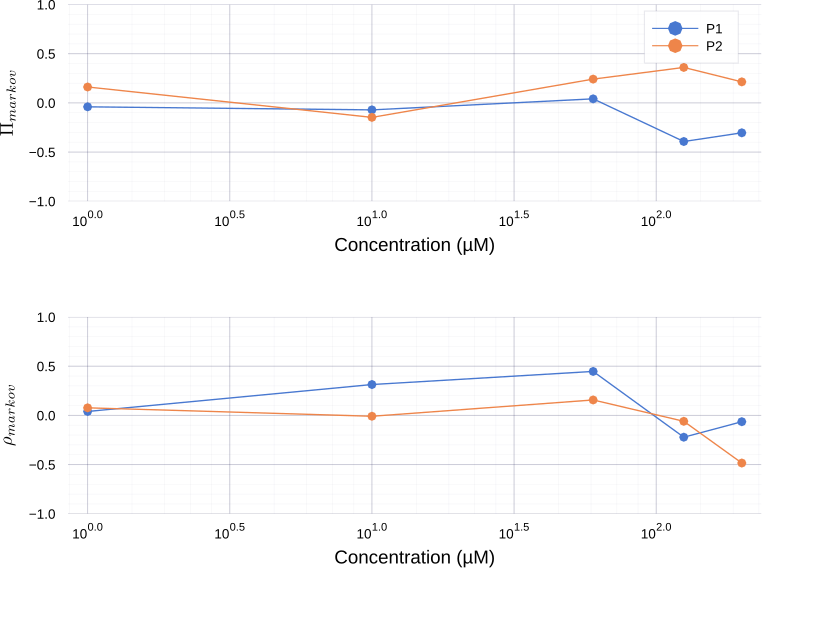
\includegraphics[width=0.8\textwidth]{part_2/assets/atp_markov.png}
      \caption{\textbf{ATP: Markov chain analysis for juveniles} \textbf{Top}: Mean Markov-based preference index (equation~\ref{mean_pi_markov}). \textbf{Bottom}: Mean Markov ratio exploration-exploitation (equation~\ref{mean_r_markov}).}
      \label{atp_markov}
    \end{figure}

  \chapter{Preference index distributions}
    \begin{figure}[h]
      \centering
      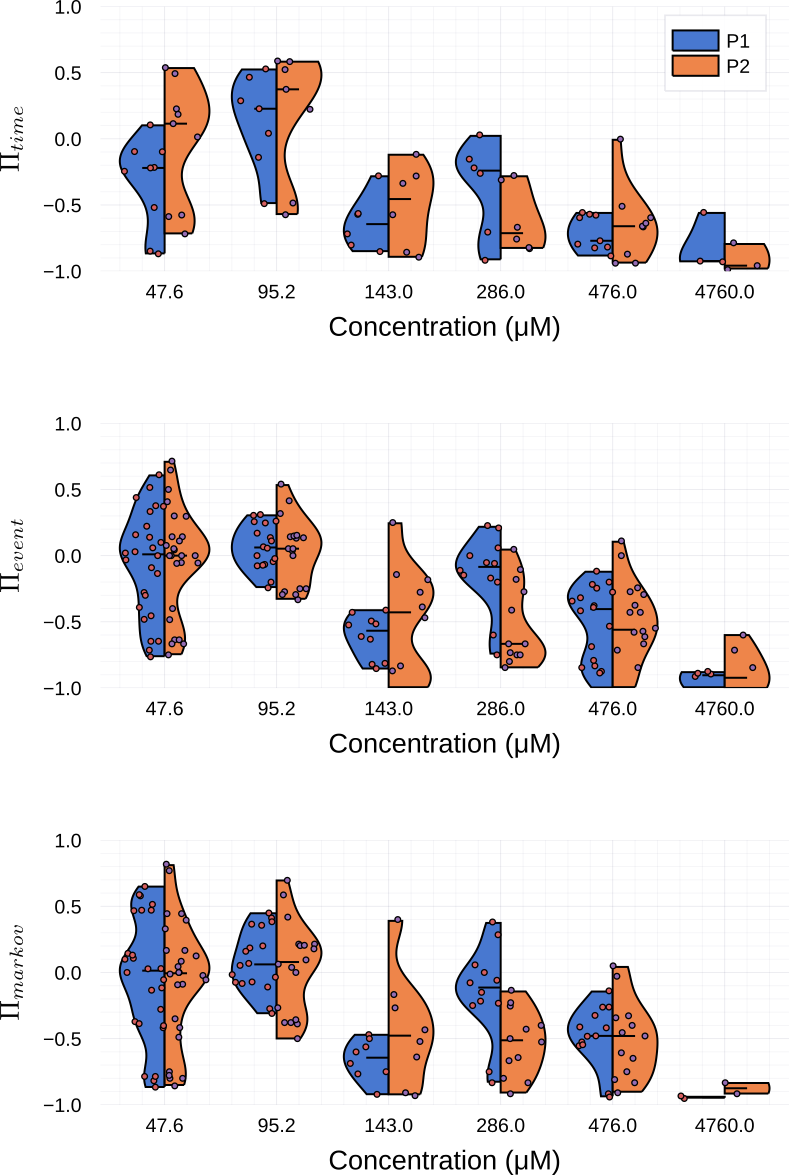
\includegraphics[width=0.8\textwidth]{part_2/assets/dist_citricacid.png}
      \caption{\textbf{Citric acid: preference index for juveniles} Event-based preference index $\Pi_{time}$, one point is one fish (top). Event-based preference index $\Pi_{event}$, one point is one fish analyzed by one person (middle). Event-based preference index $\Pi_{Markov}$, one point is one fish analyzed by one person (bottom).}
      \label{dist_citric_acid}
    \end{figure}
    \begin{figure}[h]
      \centering
      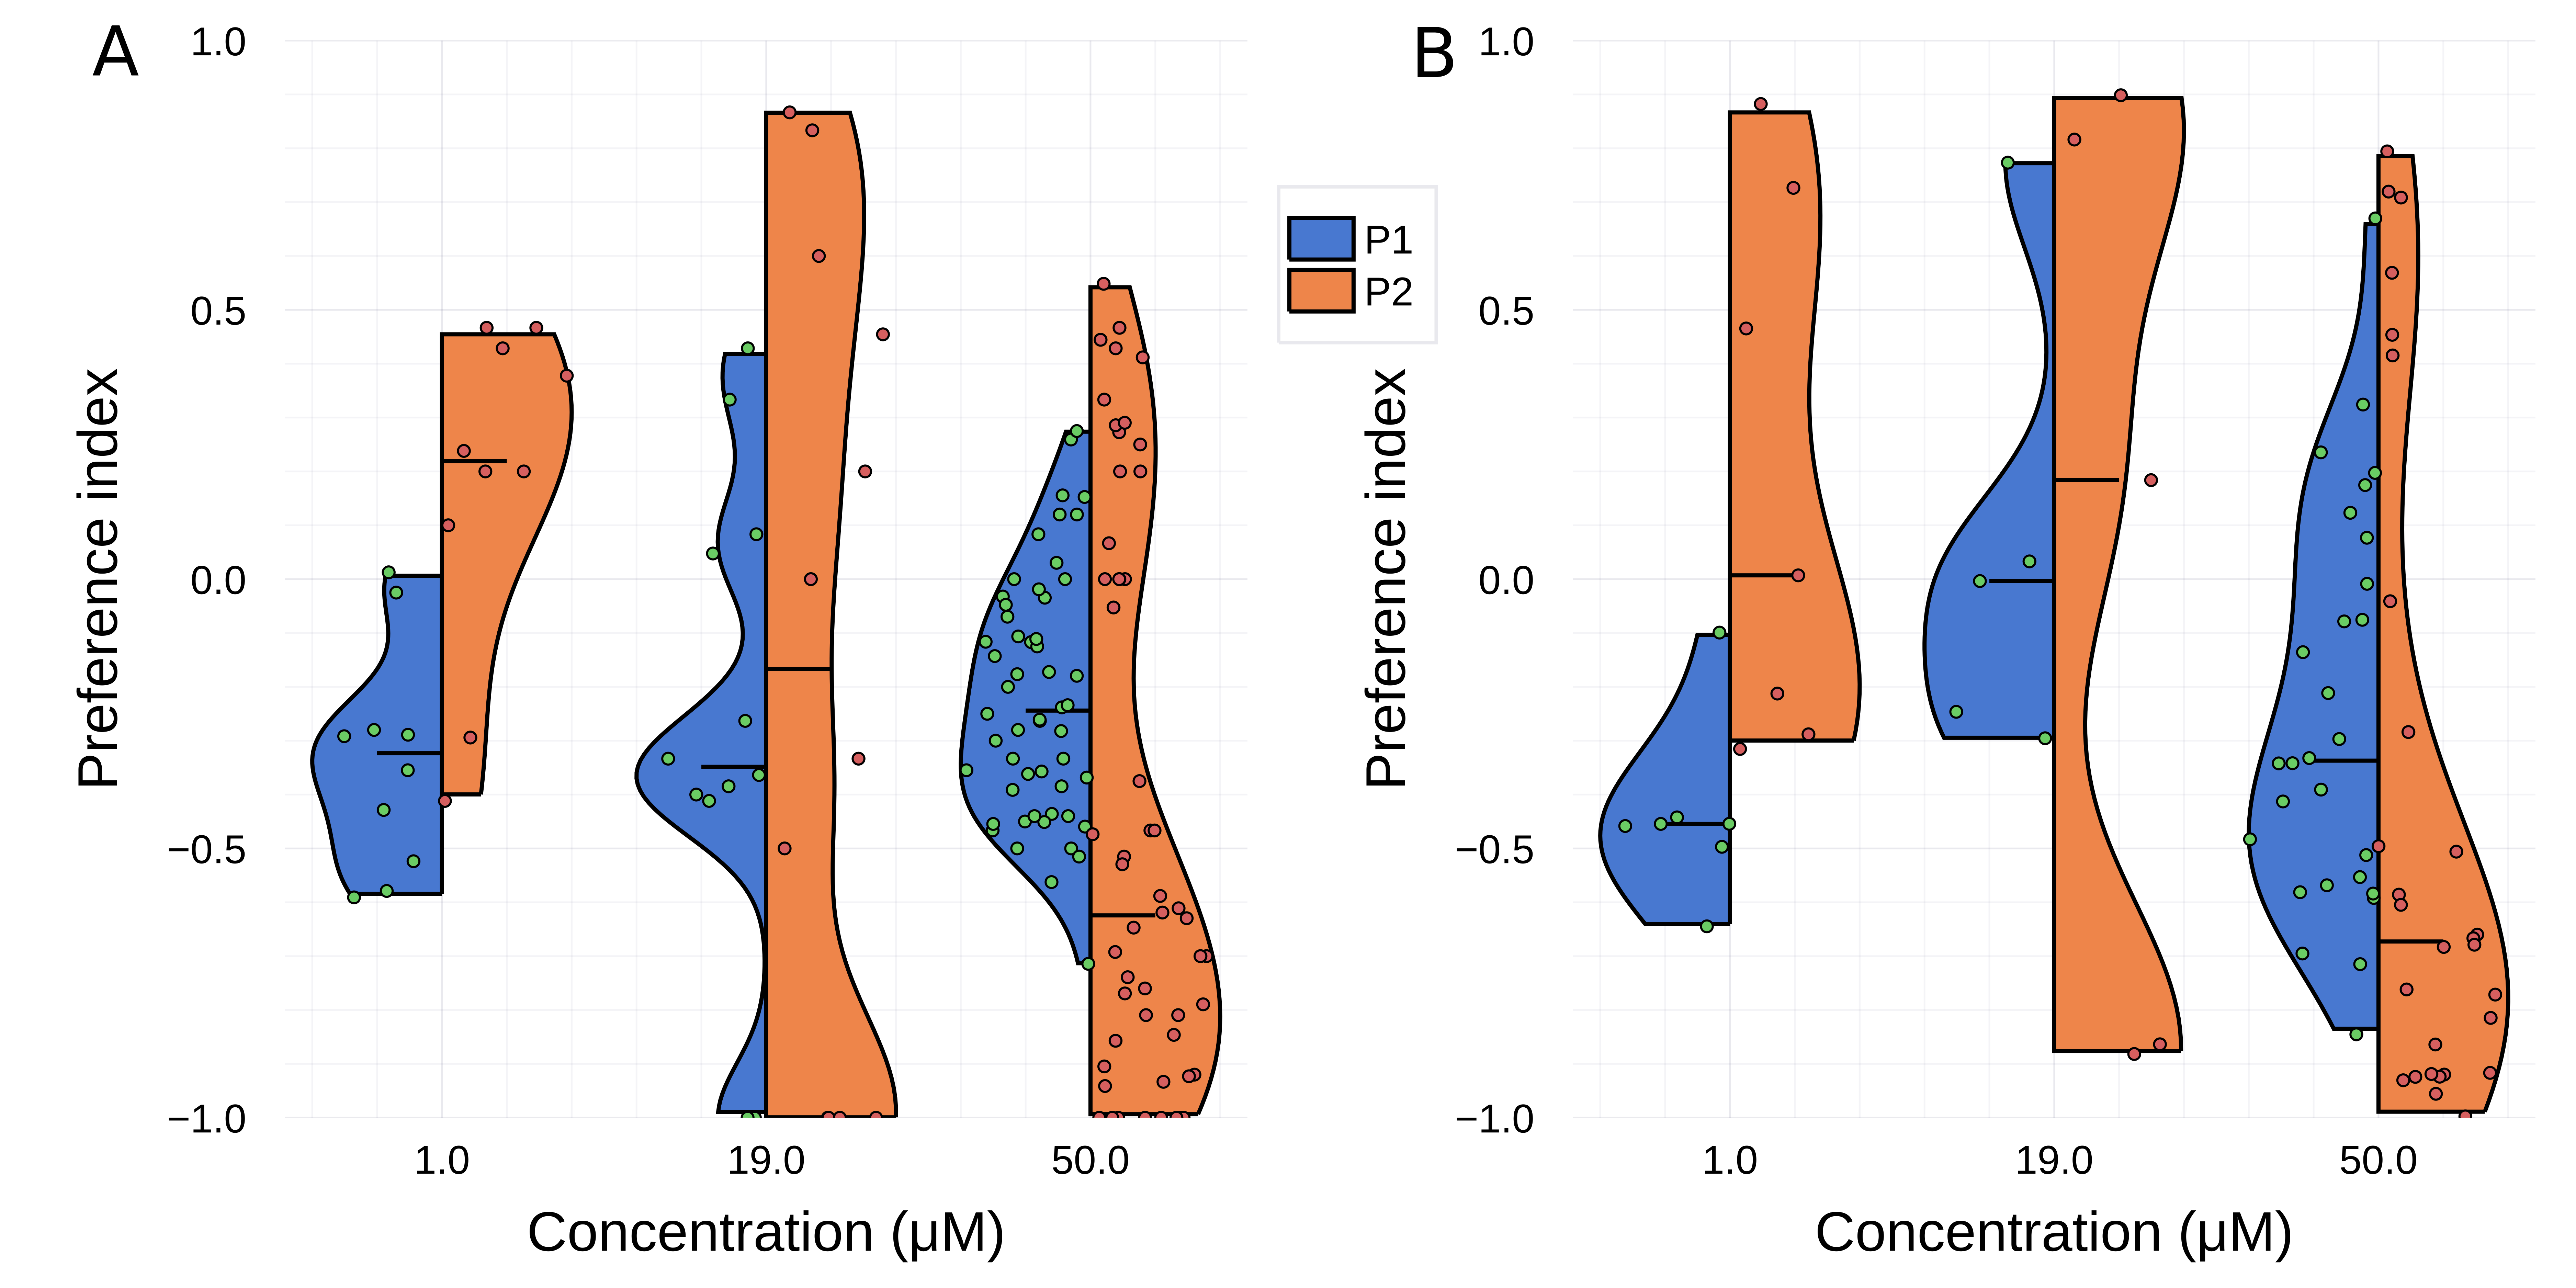
\includegraphics[width=0.8\textwidth]{part_2/assets/dist_adenosine.png}
      \caption{\textbf{Adenosine: preference index for juveniles} Event-based preference index $\Pi_{time}$, one point is one fish (top). Event-based preference index $\Pi_{event}$, one point is one fish analyzed by one person (middle). Event-based preference index $\Pi_{Markov}$, one point is one fish analyzed by one person (bottom).}
      \label{dist_adenosine}
    \end{figure}
    \begin{figure}[h]
      \centering
      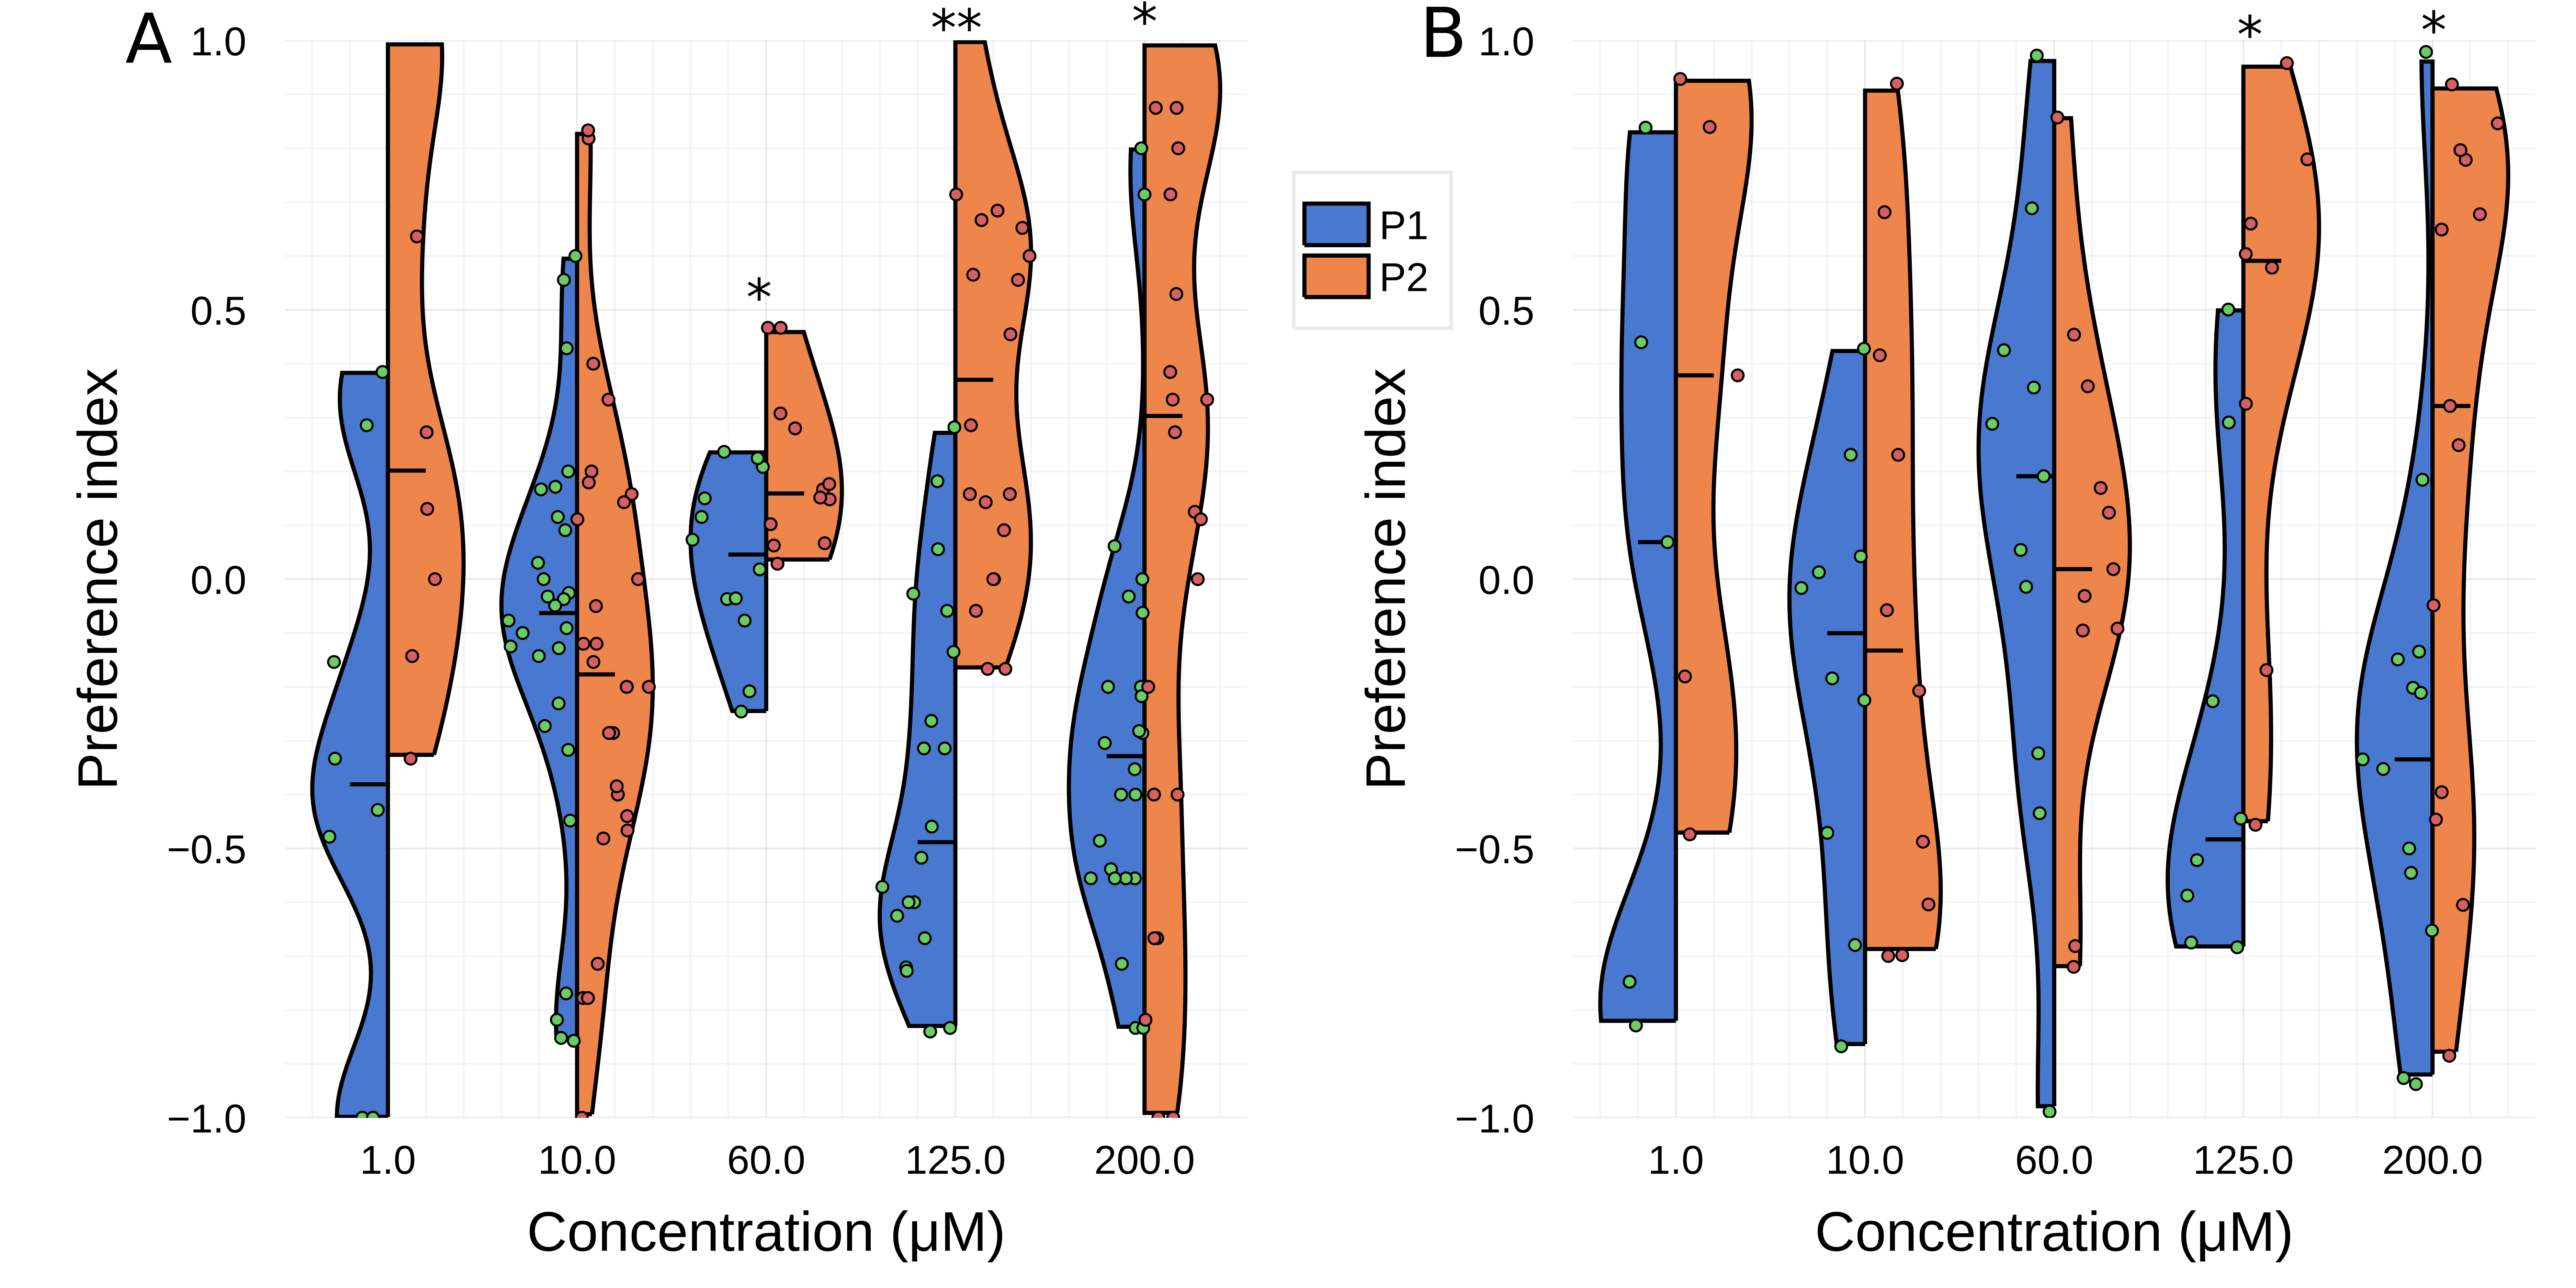
\includegraphics[width=0.8\textwidth]{part_2/assets/dist_atp.png}
      \caption{\textbf{ATP: preference index for juveniles} Event-based preference index $\Pi_{time}$, one point is one fish (top). Event-based preference index $\Pi_{event}$, one point is one fish analyzed by one person (middle). Event-based preference index $\Pi_{Markov}$, one point is one fish analyzed by one person (bottom). * $P<0.05$, ** $P<0.01$}
      \label{dist_atp}
    \end{figure}

\end{appendices}
